\documentclass[compress]{beamer}

% TODO: Add slide about monomial representation, as an example intro to object oriented programming.
% TODO: Add slide describing that the basis pre-computes weak gradients and inner products for its
%       elements on each oriented shape face.

% define binary div operator
\makeatletter
\newcommand*{\bdiv}{%
  \nonscript\mskip-\medmuskip\mkern5mu%
  \mathbin{\operator@font div}\penalty900\mkern5mu%
  \nonscript\mskip-\medmuskip
}
\makeatother

\let\Tiny=\tiny % Gets rid of font warning.
\usepackage{lmodern,amsmath,amssymb,listings}
\usepackage{spot}
\usepackage{fancybox}
\usepackage[skins,listings]{tcolorbox}
\tcbset{enhanced}
\usepackage{fancyvrb}
\usepackage[latin1]{inputenc}
\usepackage[T1]{fontenc}
\usetheme{Warsaw}
\setbeamertemplate{navigation symbols}{} % turn off slide navigation buttons at the bottom
\setbeamersize{text margin left=6mm, text margin right=6mm} 

\title[Implementing WGFEM]{Implementing the Weak Galerkin F.E.M.}
\subtitle{With a Focus on Generality}

\author{Stephen Harris \\ \texttt{scharris@ualr.edu}}
\date{Nov. 7, 2013}


\begin{document}

\begin{frame}
  \titlepage
\end{frame}

\begin{frame}
  \frametitle{Outline}
  \tableofcontents[pausesections]
\end{frame}

\section{Generality Goal}
\subsection{Generality Defined}

\begin{frame}
  \frametitle{What is Meant by Generality Here?}
  \pause
  The ability to most easily solve the widest variety of problems
    \begin{align*}
      \spot<7>{\mathfrak{a}}(u_h,v) & = (\spot<4>{f},v)\quad\quad\quad \forall{v} \in \spot<6>{V_{h0}} \\
      u_h & = Q_b \spot<4>{g} \text{ on } \partial\spot<5>{\Omega}
    \end{align*}
    for solution $u_h$ in piecewise polynomial approximation space $V_h$ on mesh \spot<5>{$M_h$} of \spot<5>{$\Omega$}.
  \pause

  \begin{block}{Method Should Allow ``Mix and Match'' of Parts}
    Should allow the ``actors'' above to easily be varied independently:
    \pause
    \begin{enumerate}[<+->]
      \item functions $f$ and $g$
      \item mesh $M_h$ on which $V_h$ members are piecewise polynomial
      \item approximation space, by choice of \emph{degree constraints} on polynomial pieces of $V_h$ members -- by monomial degree or maximum variable degree
      \item bilinear form $\mathfrak{a}: V_h \times V_h \rightarrow \mathbb{R}$
    \end{enumerate}
  \end{block}

\end{frame}

\begin{frame}
  \frametitle{How General is the Implementation?}
  \pause
  \begin{itemize}[<+->]
    \item Many problems solvable without code additions or changes.
      \begin{itemize}[<+->]
        \item Allow arbitrary functions for $f$ and $g$.
        \item Provided Meshes
          \begin{itemize}
            \item Triangle meshes from mesh generator (Gmsh).
            \item Rectangle meshes for any number of space dimensions.
          \end{itemize}
        \item Basis -- Support arbitrary \emph{degree constraints} for approximating polynomials on interiors and sides separately,
          using either monomial or variable degree.
        \item Laplace bilinear form provided. 
      \end{itemize}
    \item Extensible in areas expected to frequently need changes.
      \begin{itemize}
        \item New problems solved by plugging in new code at \emph{plugin points}.
        \item Major plugin points are provided for
          \begin{itemize}
            \item variational bilinear form, $\mathfrak{a}$
            \item mesh -- Arbitrary polytope meshes for any space dimension can be supported. No uniformity requirements.
          \end{itemize}
        \item No mesh or vbf is ``built in'': provided ones use plugin system.
        \item Only \emph{new} aspects have to be coded for, thought about, and tested. Core method does not change.
      \end{itemize}
  \end{itemize}
\end{frame}

\subsection{The Means -- Abstraction and Modularity}

\subsubsection{Components: Limited Roles, Limited Knowledge}

\begin{frame}
  \frametitle{How? Components: Limited Roles, Limited Knowledge}
  Divide system into components having clear, limited roles.
  \pause
  \tcbset{left=1mm,right=1mm,bottom=1mm,top=1mm}
  \tcbox{Limited Role} \raisebox{3mm}{$\implies$} \raisebox{-0.2mm}{\tcbox{Limited Knowledge}}\\
  A component having a limited role means it also should have no knowledge of other components' internal workings.\\
  \pause
  Components should only depend on exposed operations of other components and their \emph{documented} behavior (usually the names).\\
  \pause
  Keep connections between components at a minimum!
  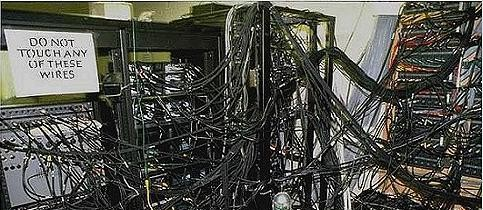
\includegraphics[height=3.5cm]{img/crazy-wiring.jpg}
\end{frame}

\subsubsection{Components for the WG Method}

\begin{frame}
  \frametitle{How Generality is Achieved: Abstraction and Modularity}
  Divide system into components having clear, limited roles.\\
  \pause
  \tcbset{colback =red!5!white, colframe =red!75!black, left=0mm,right=0mm,bottom=0mm,top=0mm}
  \begin{block}{Major Components}
    \tcbox{\shadowbox{Mesh}}
    \raisebox{1.4mm}{\shadowbox{WGrad Solver}}
    \raisebox{1.4mm}{\shadowbox{Basis}}
    \raisebox{1.25mm}{\shadowbox{Proj}}
    \tcbox{\shadowbox{VBF}}
    \raisebox{3.4mm}{\fbox{WG Solver}}
  \end{block}
  \pause
  \begin{block}{Auxiliary Types \& Components}
    \shadowbox{Monomial}
    \shadowbox{Polynomial}
    \shadowbox{Vector Monomial}
    \shadowbox{Weak Grad}
    \shadowbox{WG Solution}
    \raisebox{2mm}{\fbox{Error Norms}}
    \raisebox{2mm}{\fbox{Quadrature}}
    \raisebox{2mm}{\fbox{Linear Algebra}}
  \end{block}
  \pause
  \raisebox{-2mm}{\shadowbox{Shadowed}} components represent \emph{types}, with custom ops.\\
  \pause
  \raisebox{-2mm}{\tcbox{Enclosed}} types represent abstract
  types, or \emph{contracts}, as a set of operations which actual ``plugged in'' types must implement.
\end{frame}

\subsection{Bringing Components Together - Example}

\begin{frame}[fragile]{Bringing Components Together -- Example Run}
  \tcbset{colback =red!5!white, colframe =red!75!black, left=0mm,right=0mm,bottom=0mm,top=0mm, tcbox raise base}
  \begin{Verbatim}[gobble=4, commandchars=\\\{\}, fontsize=\small, fontfamily=tt]
    fn u(x: &[R]) -> R  \{ cos(x[0]) + sin(x[1]) \} \textcolor{gray}{// exact solution}
    fn f(x: &[R]) -> R  \{ cos(x[0]) + sin(x[1]) \} \textcolor{gray}{// var form rhs}
    fn g(x: &[R]) -> R  \{ u(x) \} \textcolor{gray}{                 // boundary cond}

    let \textcolor{green!50!black}{mesh} = \spot{~RectMesh}::new(~[0.,0.], ~[2*pi,2*pi], ~[500, 500]);

    let \textcolor{blue}{basis} = &WGBasis::new(\tcbox{\textcolor{green!50!black}{mesh}}, MaxMonDeg(3), MaxMonDeg(2));

    let \textcolor{orange!50!red}{vbf} = \spot{VBFLaplace}::new(None, \textcolor{blue}{basis});

    let wg_sol = wg_solver::solve(\tcbox{\textcolor{orange!50!red}{vbf}}, \textcolor{blue}{basis}, f, g);

    let err = err_L2_norm(u, &wg_sol);
  \end{Verbatim}
  \footnotesize {
    \textcolor{gray}{// \spot{\emph{Any} types satisfying the respective contracts are usable at these spots.}}\\
    \textcolor{gray}{// The types are only manipulated via contract-guaranteed operations within\\
      // the method -- black boxes with contract ops being the external controls.}
  }
\end{frame}


\begin{frame}[fragile]
  \frametitle{Creating Types}
  \begin{itemize}[<+->]
    \item A \emph{type} consists of some data bundled together seamlessly with the operations that act on the data.  The operations
      always come along with the data, when instances of the type are passed around between functions.  Given an \emph{instance} or
      \emph{object} named \textcolor{blue}{\small \texttt{someObject}} of a given type where the data is contained, operations on the
      type are normally denoted \textcolor{blue}{\small \texttt{someObject.\textbf{\textcolor{orange}{someFunction}}(arg1,\dots,argN)}}.

    \item We saw this above, where objects representing a mesh, a basis, and a vbf were created. It should be apparent
      that the operations must come along with these objects, because the WG method only receives these objects to its solve function,
      and yet somehow also must be getting the operations for the specific mesh and VBF.
      \tcbset{colback =red!5!white, colframe =red!75!black, left=0mm,right=0mm,bottom=0mm,top=0mm, tcbox raise base}
      \begin{Verbatim}[gobble=6, commandchars=\\\{\}, fontsize=\scriptsize, fontfamily=tt]
        let \textcolor{green!50!black}{mesh} = ~RectMesh::new(~[0.,0.], ~[2*pi,2*pi], ~[500, 500]);
        let \textcolor{blue}{basis} = &WGBasis::new(\tcbox{\textcolor{green!50!black}{mesh}}, MaxMonDeg(3), MaxMonDeg(2));
        let \textcolor{orange!50!red}{vbf} = VBFLaplace::new(None, \textcolor{blue}{basis});
        let wg_sol = wg_solver::solve(\tcbox{\textcolor{orange!50!red}{vbf}}, \textcolor{blue}{basis}, f, g);
      \end{Verbatim}
  \end{itemize}
\end{frame}

% TODO: Describe here how creating a new type for bundling functions and data together can be better than just calling a normal
% function with the data as first argument. The crux is that the function must either know about *all* types of data that it may
% receive (not generally possible, they may not have been written yet, ideally!), or the function itself must be passed around
% separately with the data. Which would be necessary for EACH function associated with the type, which obviously is not practical.
%\begin{frame}[fragile]
  %\frametitle{Usefulness of Types}
  %\begin{itemize}[<+->]
%\end{frame}

\section{Concepts}

\subsection{Mesh Elements}

\subsubsection{Oriented Shapes}

\begin{frame}
  \frametitle{Oriented Shapes}
  \begin{columns}
    \column{.50\textwidth}
      \frame{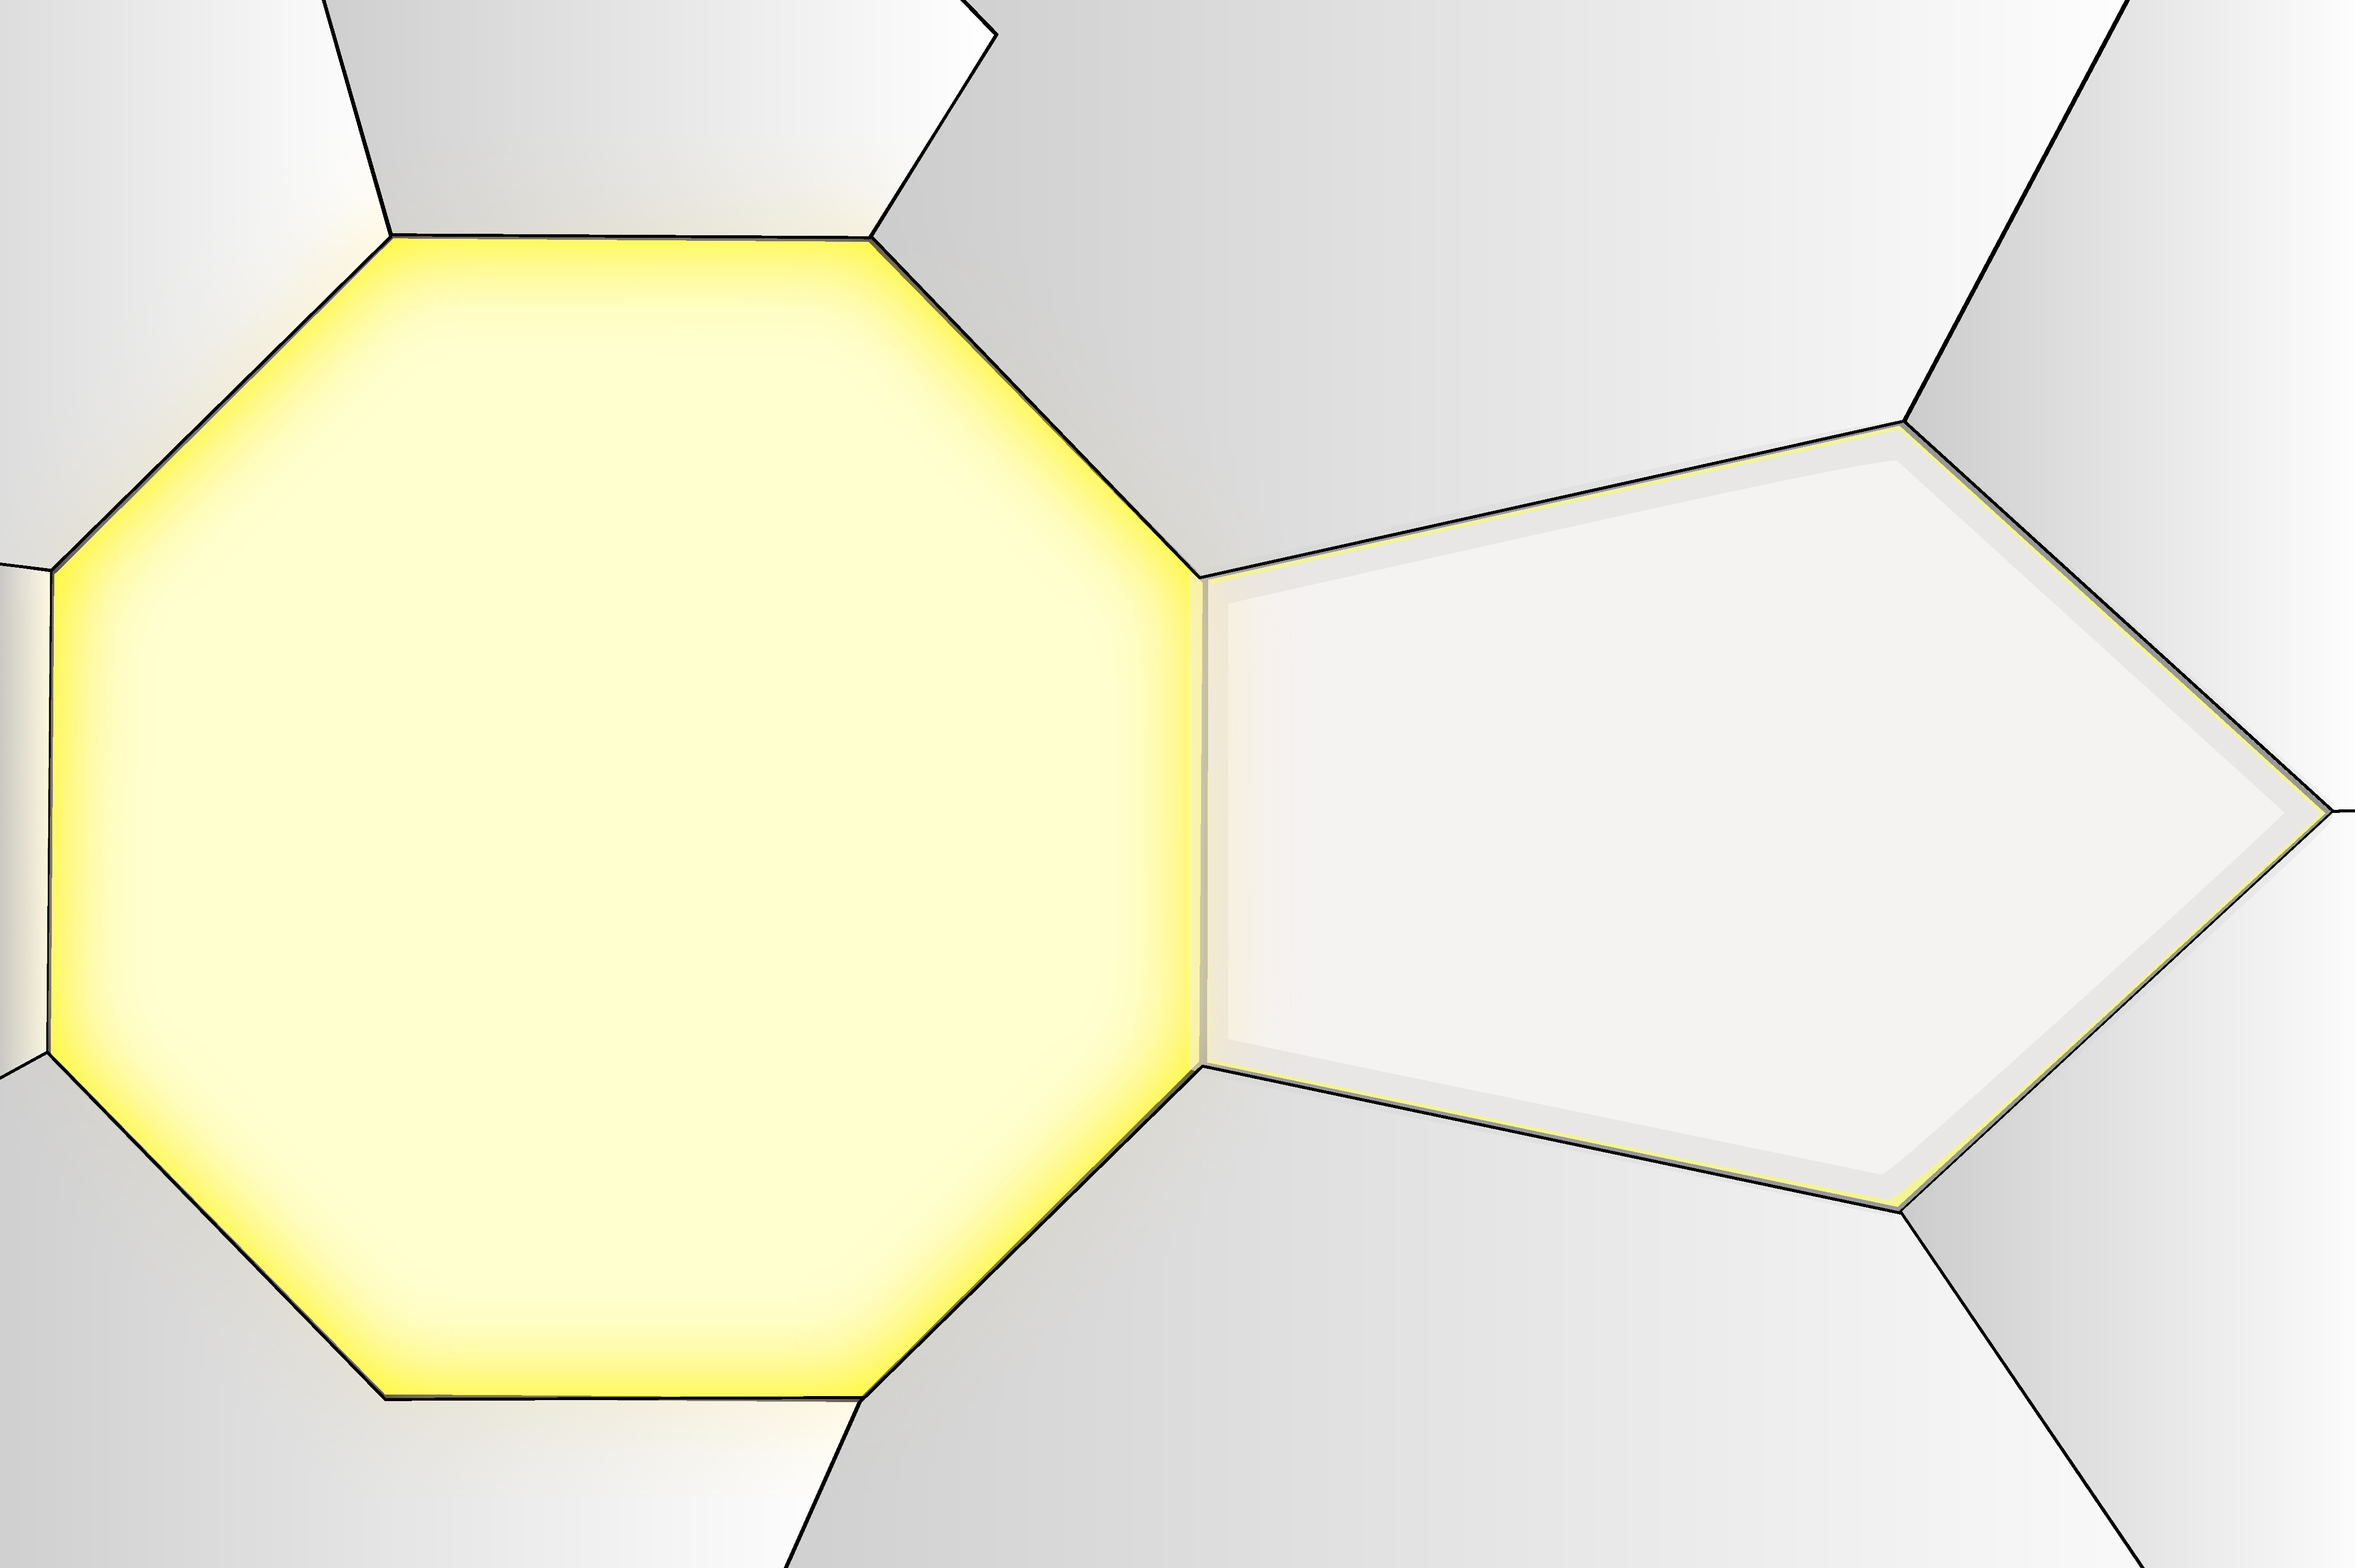
\includegraphics[width=6cm, height=4cm]{img/two_fes.pdf}}
    \column{.50\textwidth}
      \pause
      \begin{itemize}[<+->]
        \item Elements may have, \emph{independently} of each other, any \textbf{shape}, \textbf{orientation}, and \textbf{number of sides}.
        \item An \textbf{\emph{oriented shape}} is an abstraction of a finite element, ignoring its position, but including its division into
          enumerated sides.
      \end{itemize}
  \end{columns}
  
  \begin{itemize}[<+->]
    \item Formally, two elements are of the same \textbf{\emph{oriented shape}} iff the sides can be put into a one-to-one correspondence and
       there is some translation taking each side of one onto the matching side of the other.
    \item Mesh must assign an oriented shape for \emph{each} finite element. 
    \item Mesh will identify oriented shapes by enumerating them in some order of its choosing. Are just \emph{opaque} identifiers to other comps.
  \end{itemize}
\end{frame}

\subsubsection{Identifying Finite Elements and Non-Boundary Sides}

\begin{frame}
  \frametitle{Identifying Finite Elements and Non-Boundary Sides}
  \begin{columns}
    \column{.50\textwidth}
      \begin{itemize}[<+->]
        \item Mesh will need to provide identifiers for the \emph{\textbf{support faces}} for the basis shape functions.
        \item Interiors and non-boundary sides will host shape functions, so need to be identified.
      \end{itemize}
    \column{.50\textwidth}
      \alt<-2> {\frame{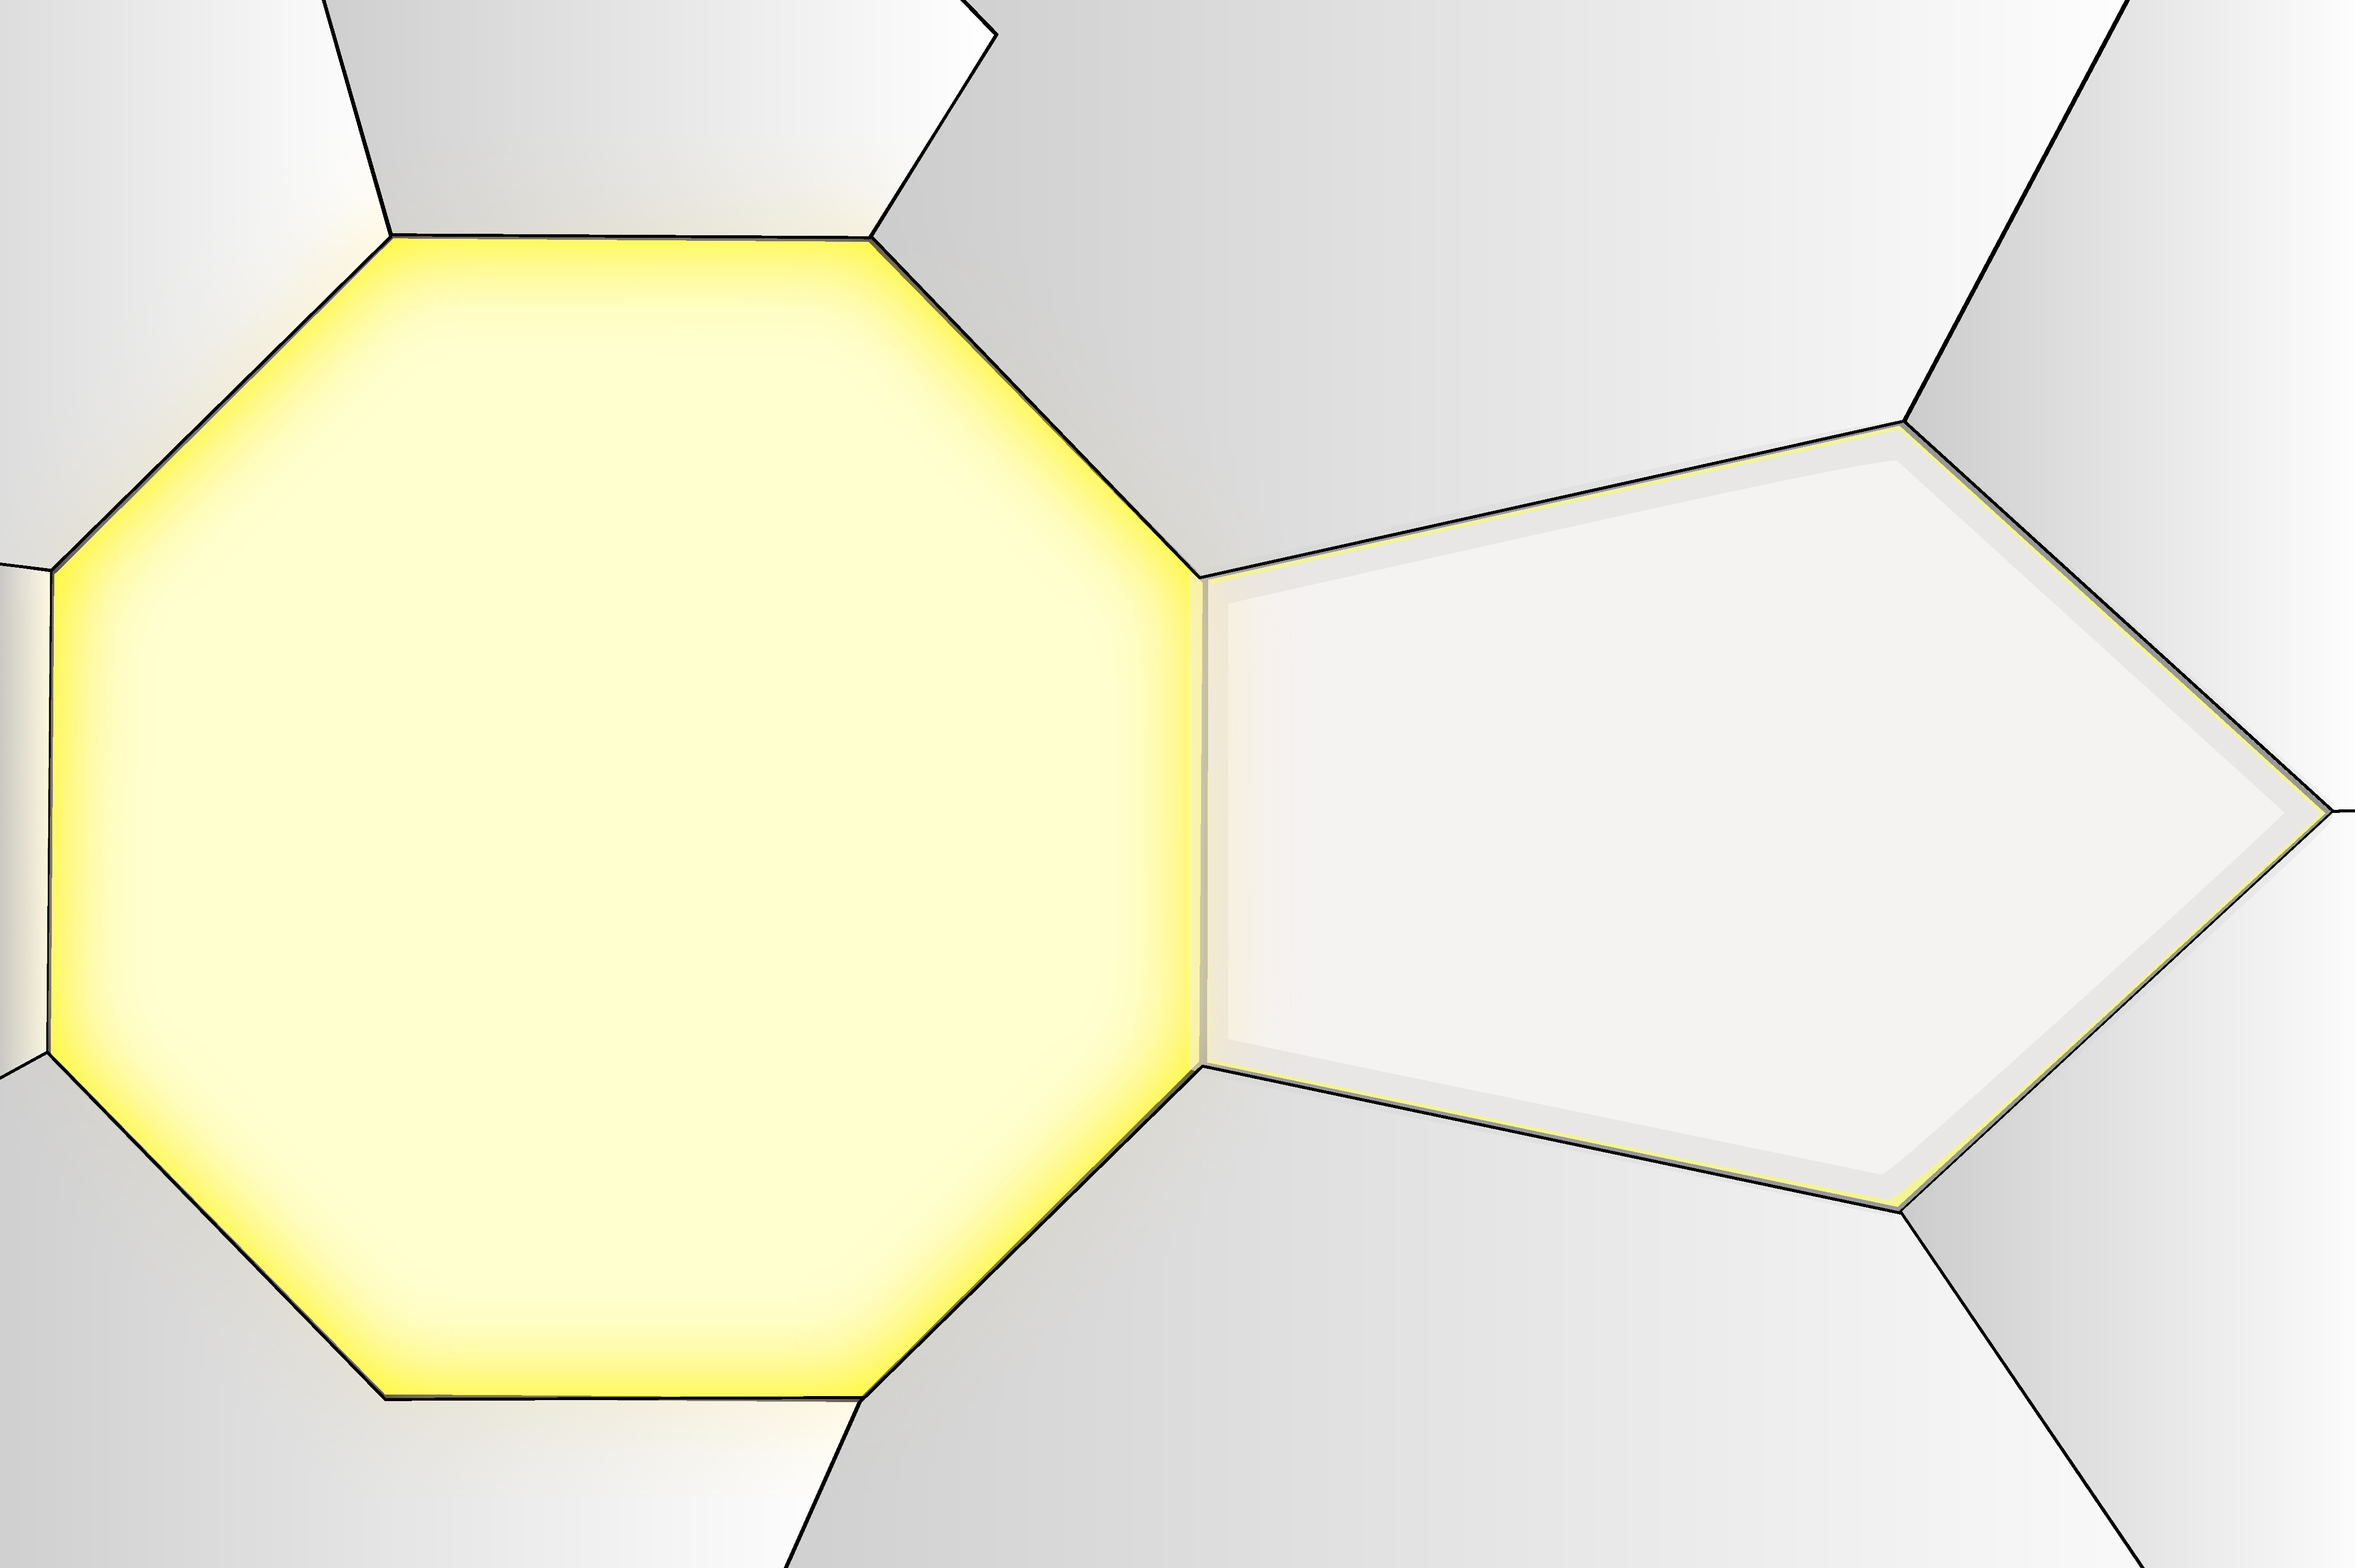
\includegraphics[width=6cm, height=4cm]{img/two_fes.pdf}}}
               {\frame{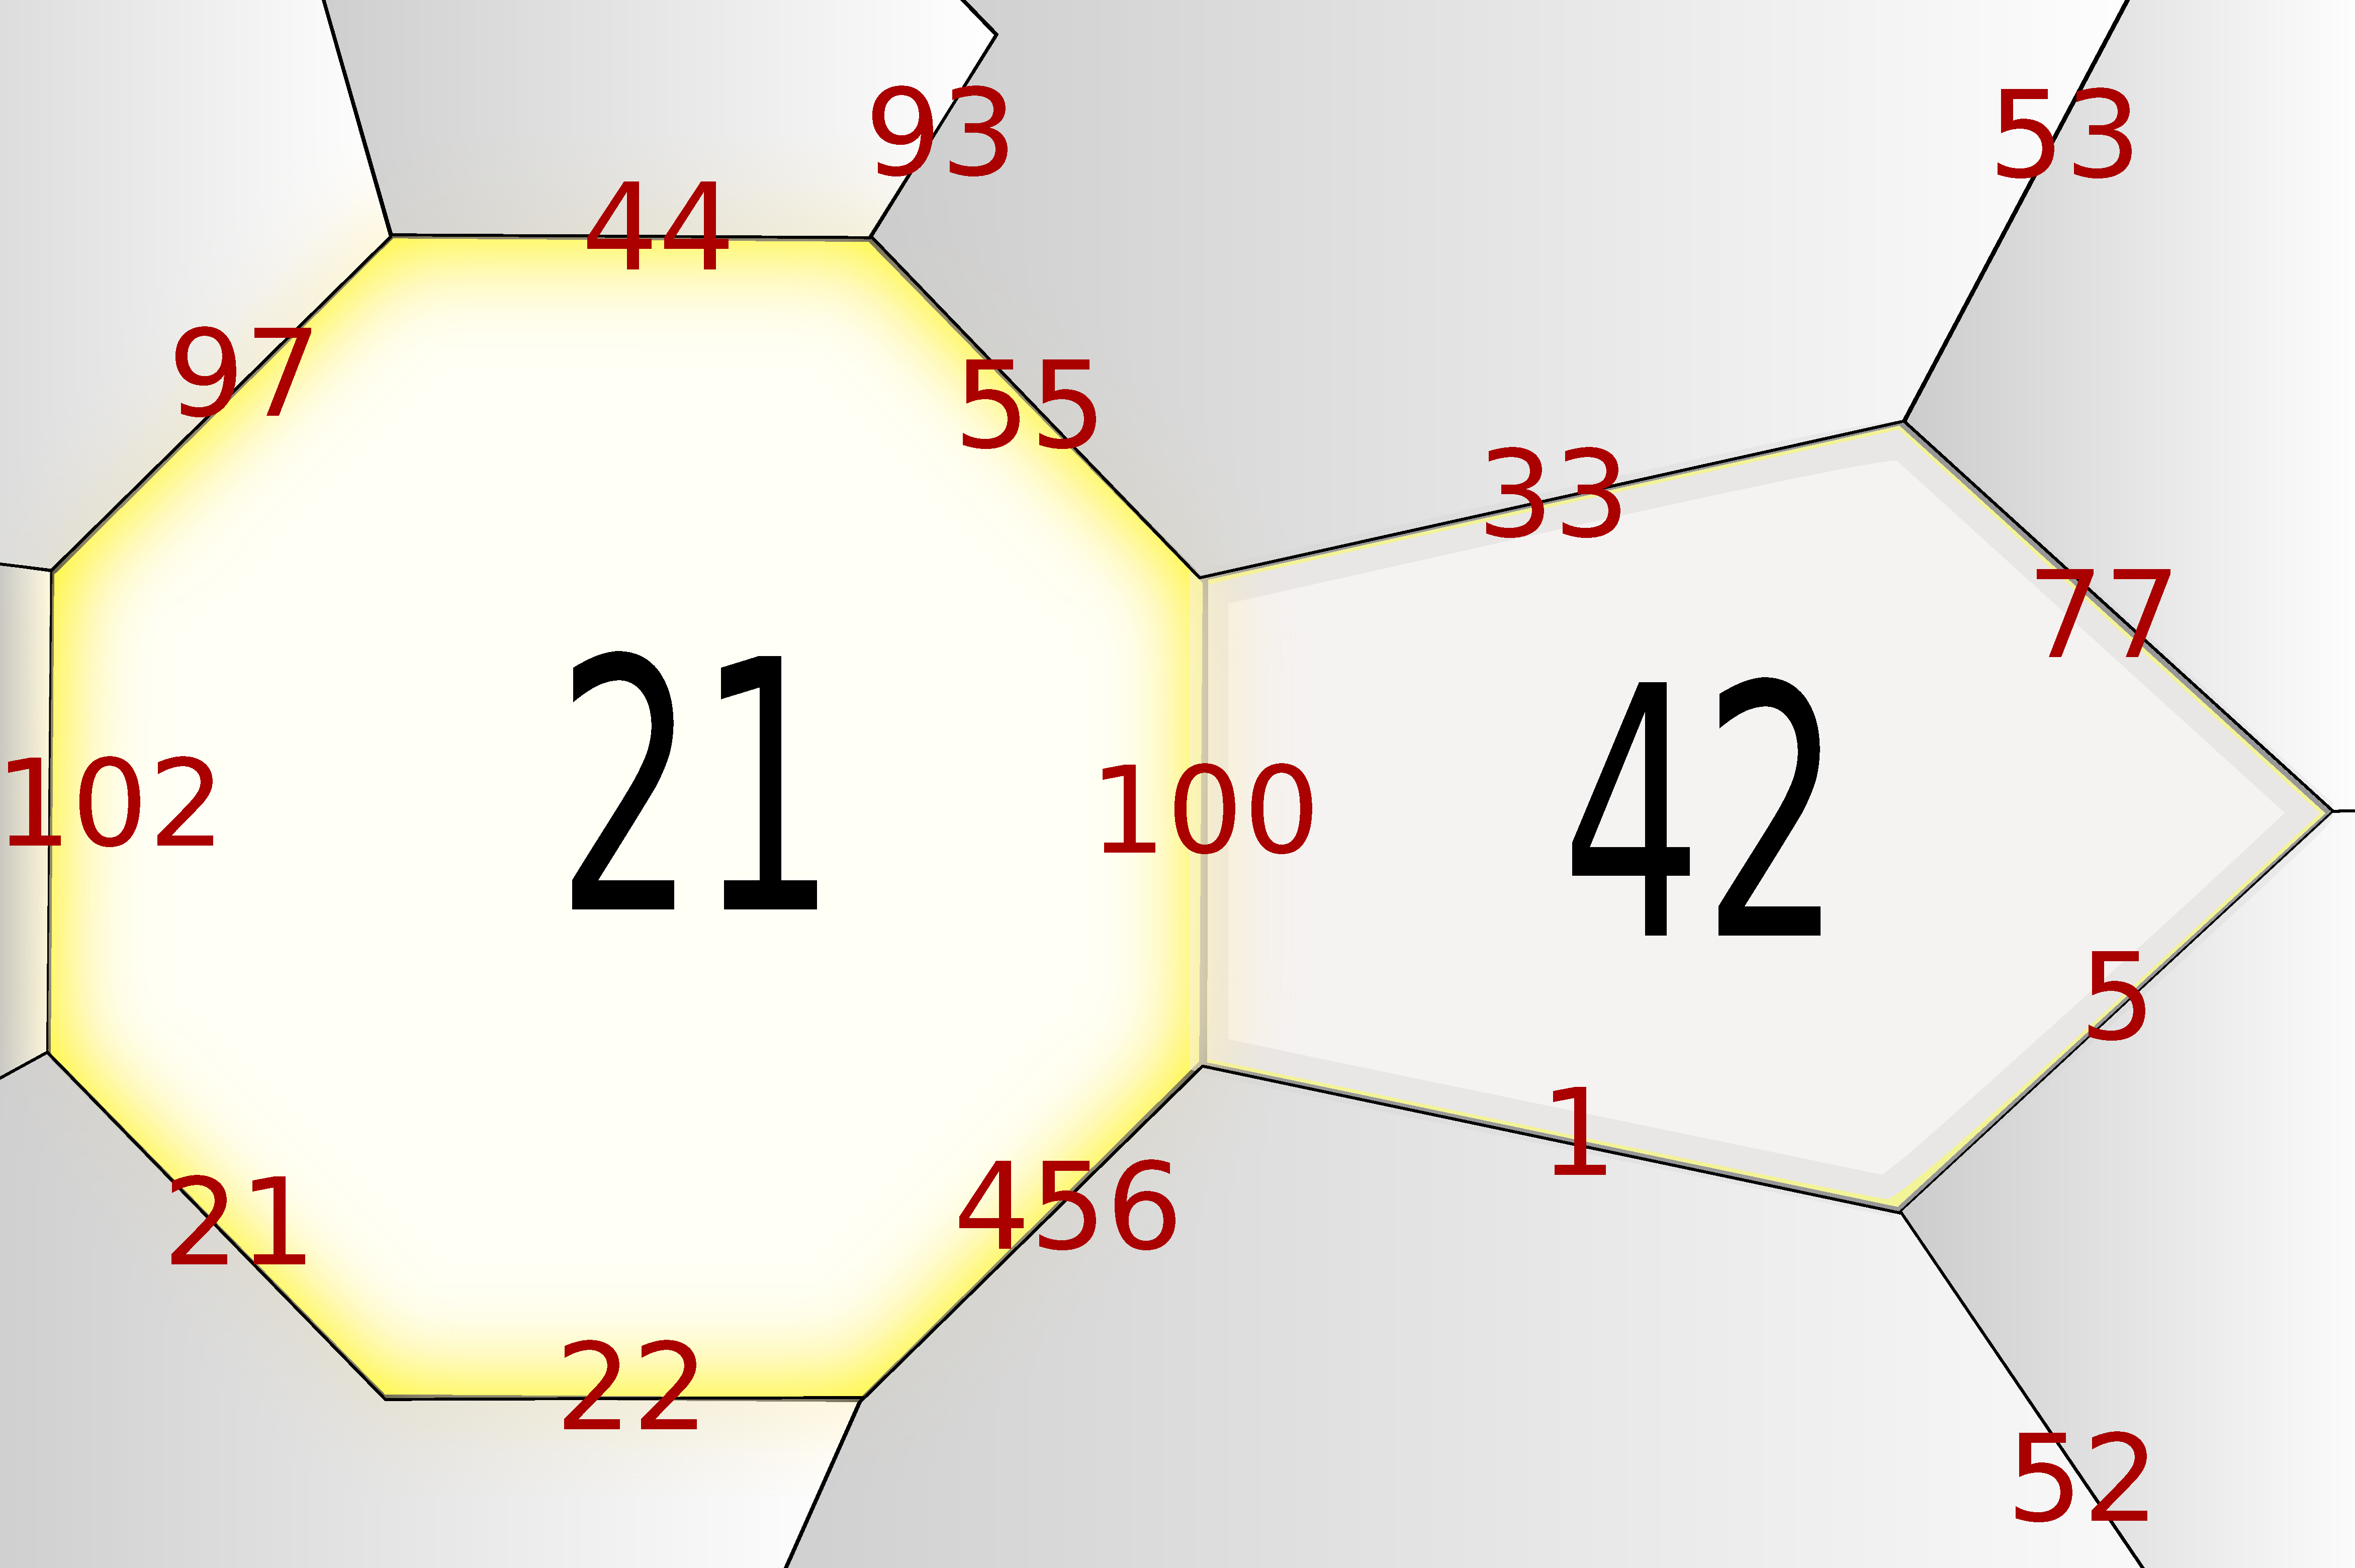
\includegraphics[width=6cm, height=4cm]{img/two_fes_enum_supp_faces.pdf}}}
  \end{columns}
  \begin{itemize}[<+->]
    \item Mesh will \textbf{enumerate finite elements (equiv., \emph{interiors}) and non-boundary sides separately}, in any order it chooses for each.
    \item Separate enumerations allow sides or fes/interiors to be dealt with separately by other components.
    \item To other components, the interior and nb side numbers are just opaque identifiers -- must ask the mesh for interpretation.
  \end{itemize}
\end{frame}
 
\subsubsection{Side Faces -- Shape Relative Side Identifiers}

\begin{frame}
  \frametitle{Side Faces -- Shape Relative Side Identifiers}
  \begin{columns}
    \column{.50\textwidth}
      \begin{itemize}[<+->]
        \item Side identifiers discussed so far are \emph{global}, and do not tell the \emph{\textbf{role}} that the side plays
          in the context of a \emph{\textbf{single oriented shape or element}}.
        \item The shape-relative side identifier is the \emph{\textbf{side face}}.
      \end{itemize}
    \column{.50\textwidth}
      \alt<-1> {\frame{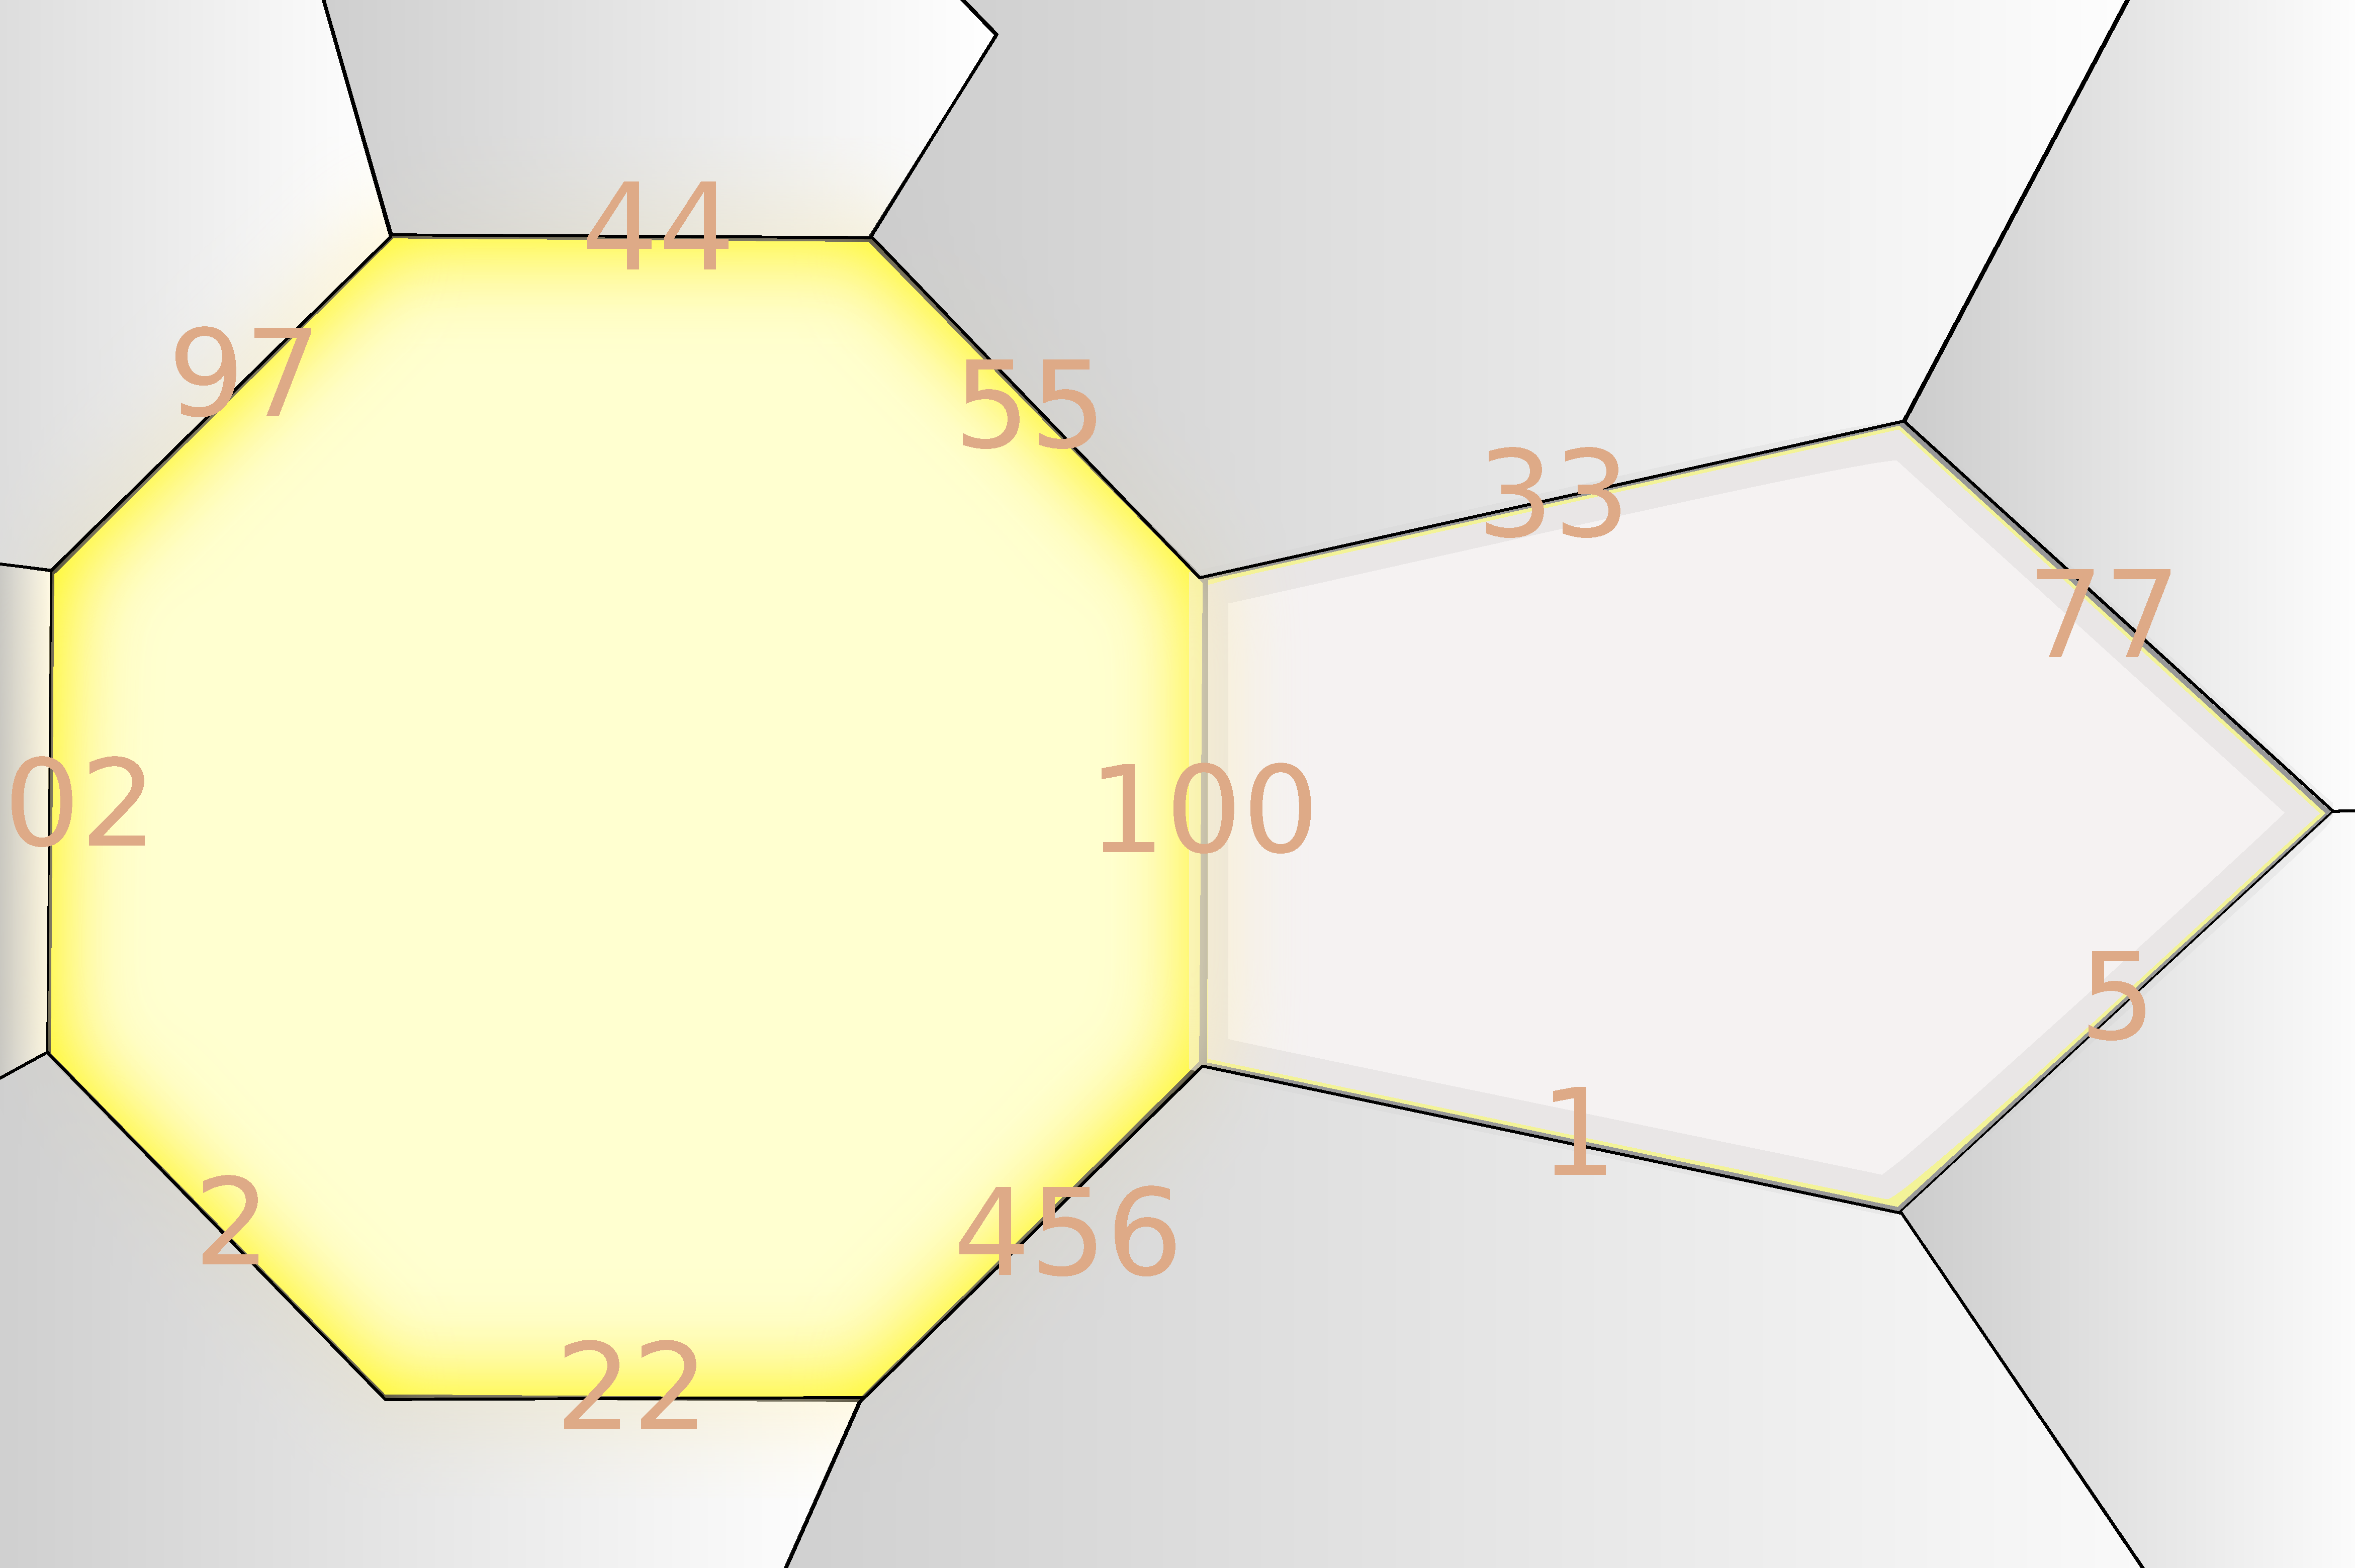
\includegraphics[width=6cm, height=4cm]{img/two_fes_enum_nb_side_nums_greyed.pdf}}}
               {\frame{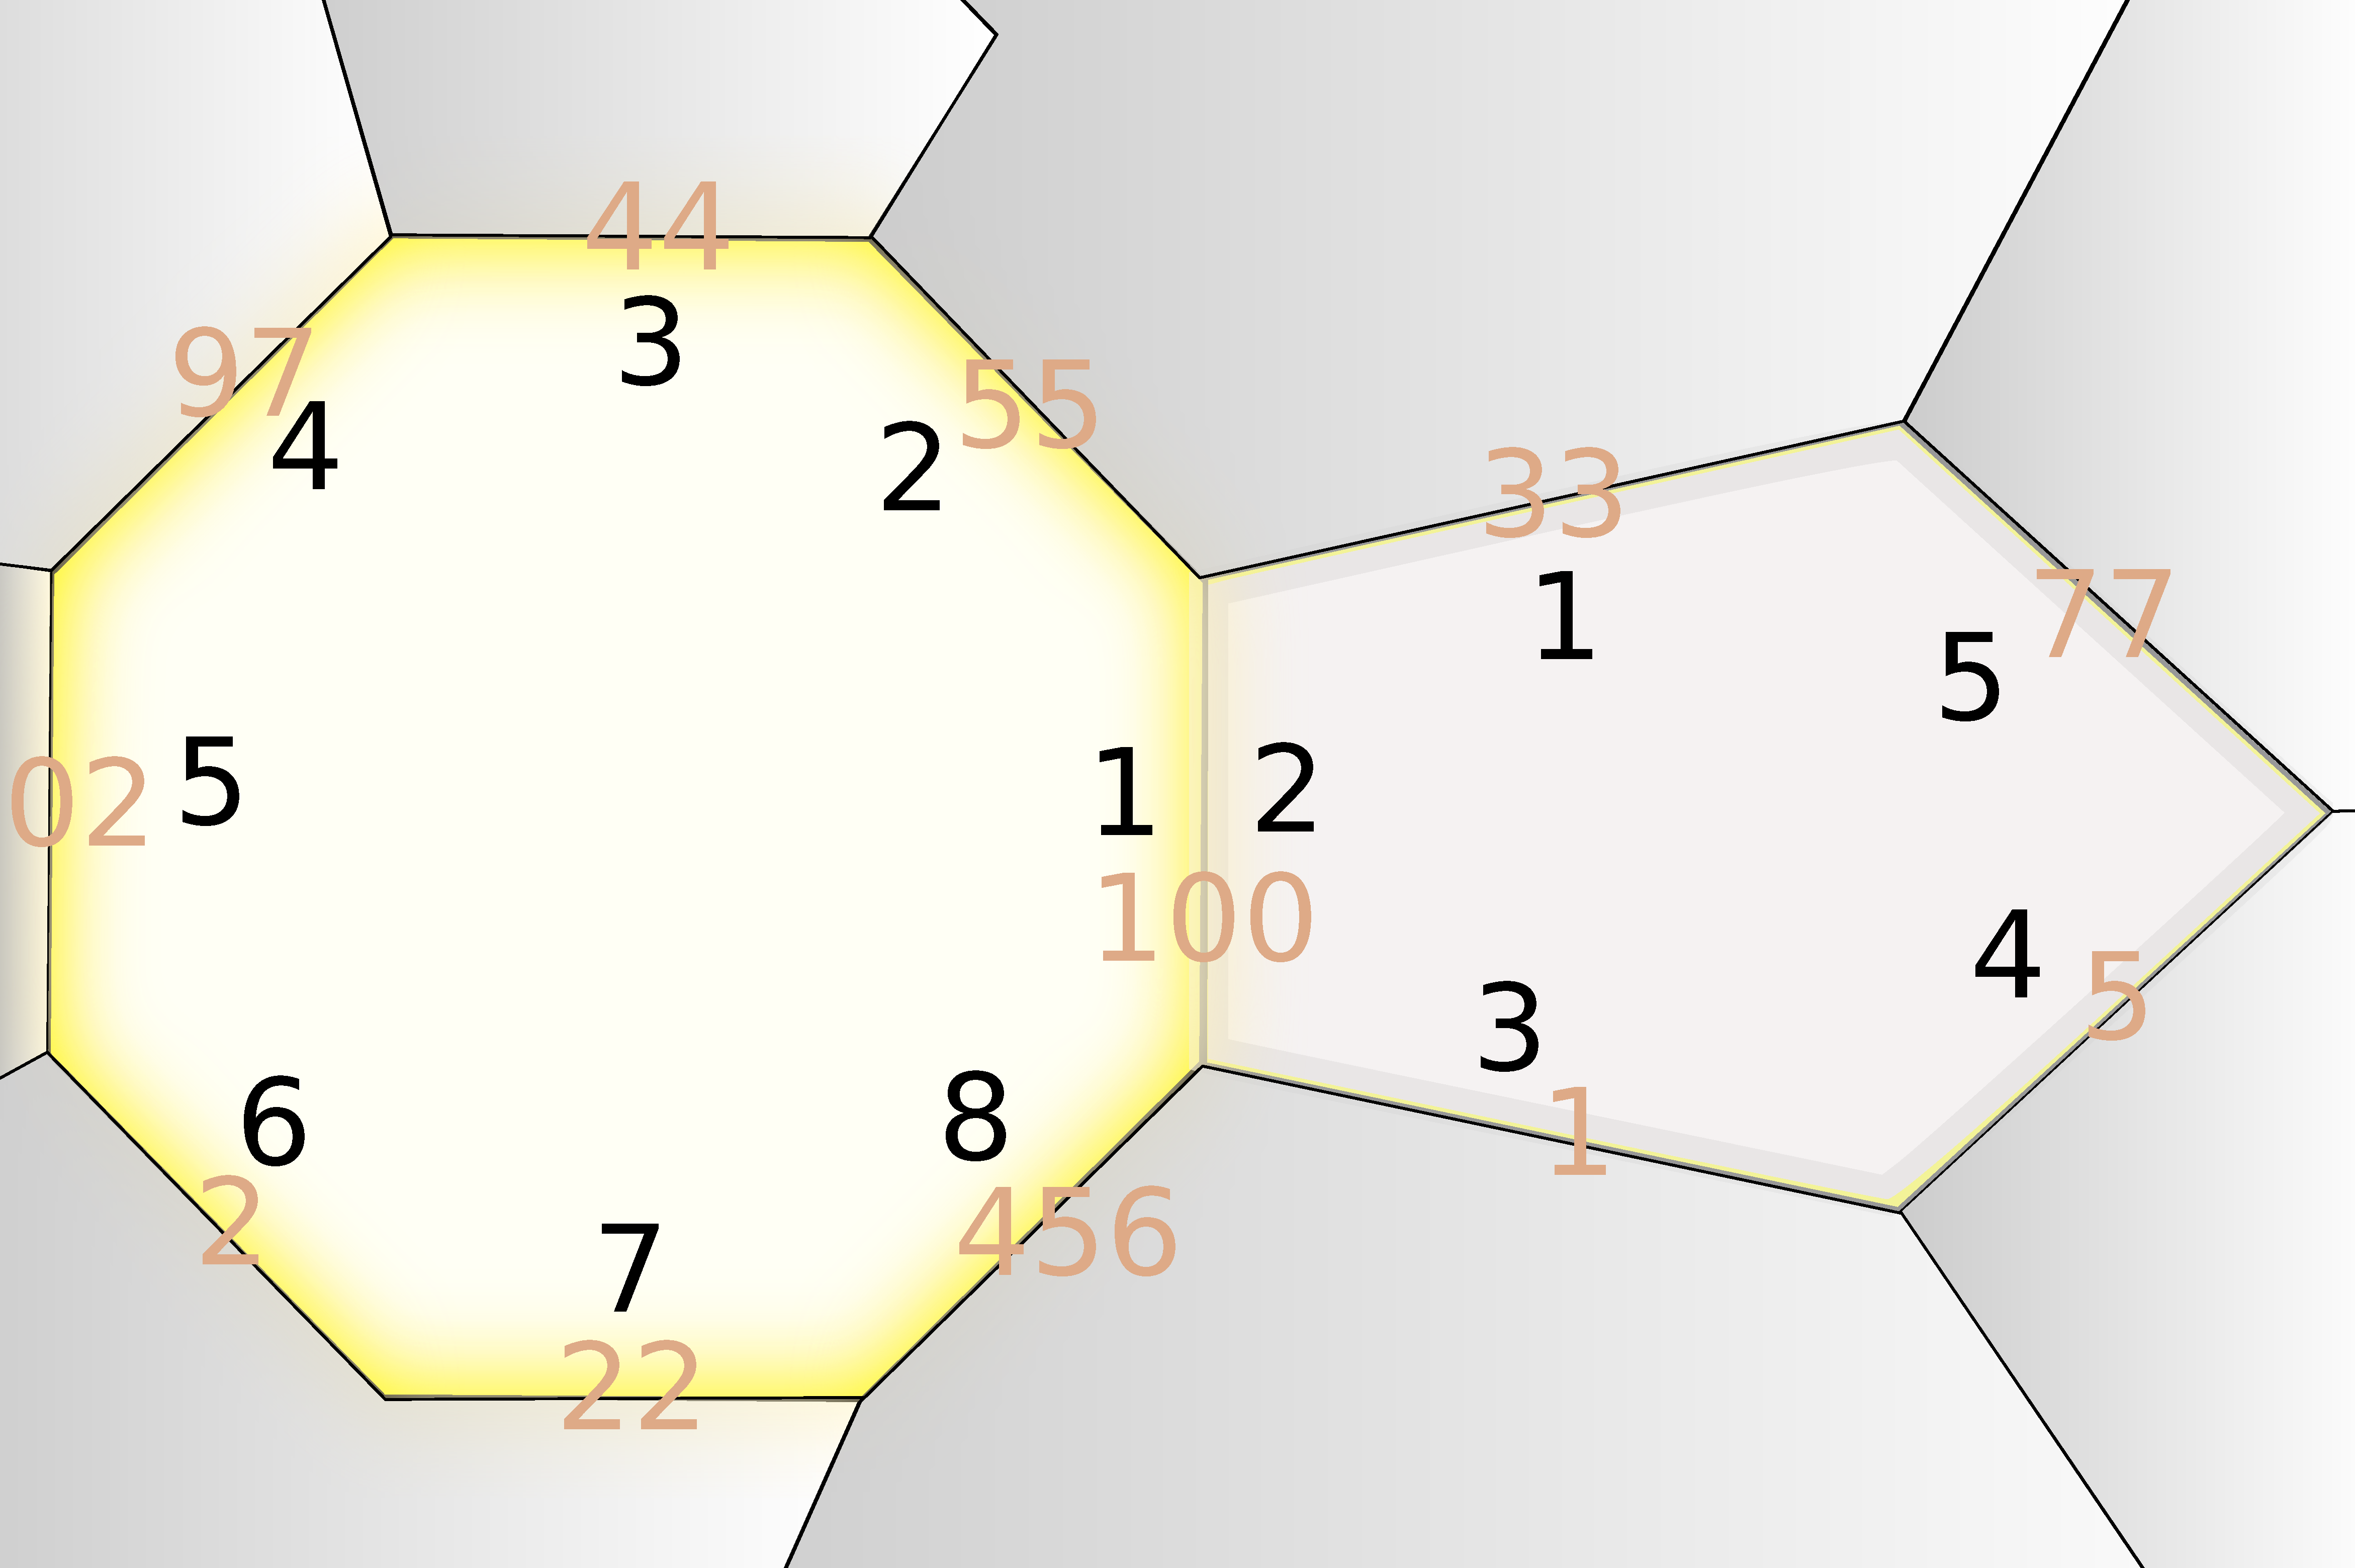
\includegraphics[width=6cm, height=4cm]{img/two_fes_enum_side_faces_nb_side_nums_greyed.pdf}}}
  \end{columns}
  \begin{itemize}[<+->]
    \item The sides may be numbered in any order by the mesh, each oriented shape having its own numbering of its side faces.
    \item A finite element inherits side face numbers from the corresponding sides of its oriented shape.
    \item Side faces are necessary to represent sides in computations involving geometry on oriented shapes and finite elements.
  \end{itemize}
\end{frame}
 
\subsubsection{Elements Including a Non-Boundary Side}

\begin{frame}
  \frametitle{Finite Elements Including a Non-Boundary Side}
  \begin{columns}
    \column{.50\textwidth}
      \begin{itemize}[<+->]
        \item Meshes will be such that each nb side is included in exactly two finite elements,
          and has no measure in any other elements.
        \item When a \emph{hanging node} divides a straight section, sections between vertexes must be separate sides.
      \end{itemize}
    \column{.50\textwidth}
    \alt<-1> {
        \frame{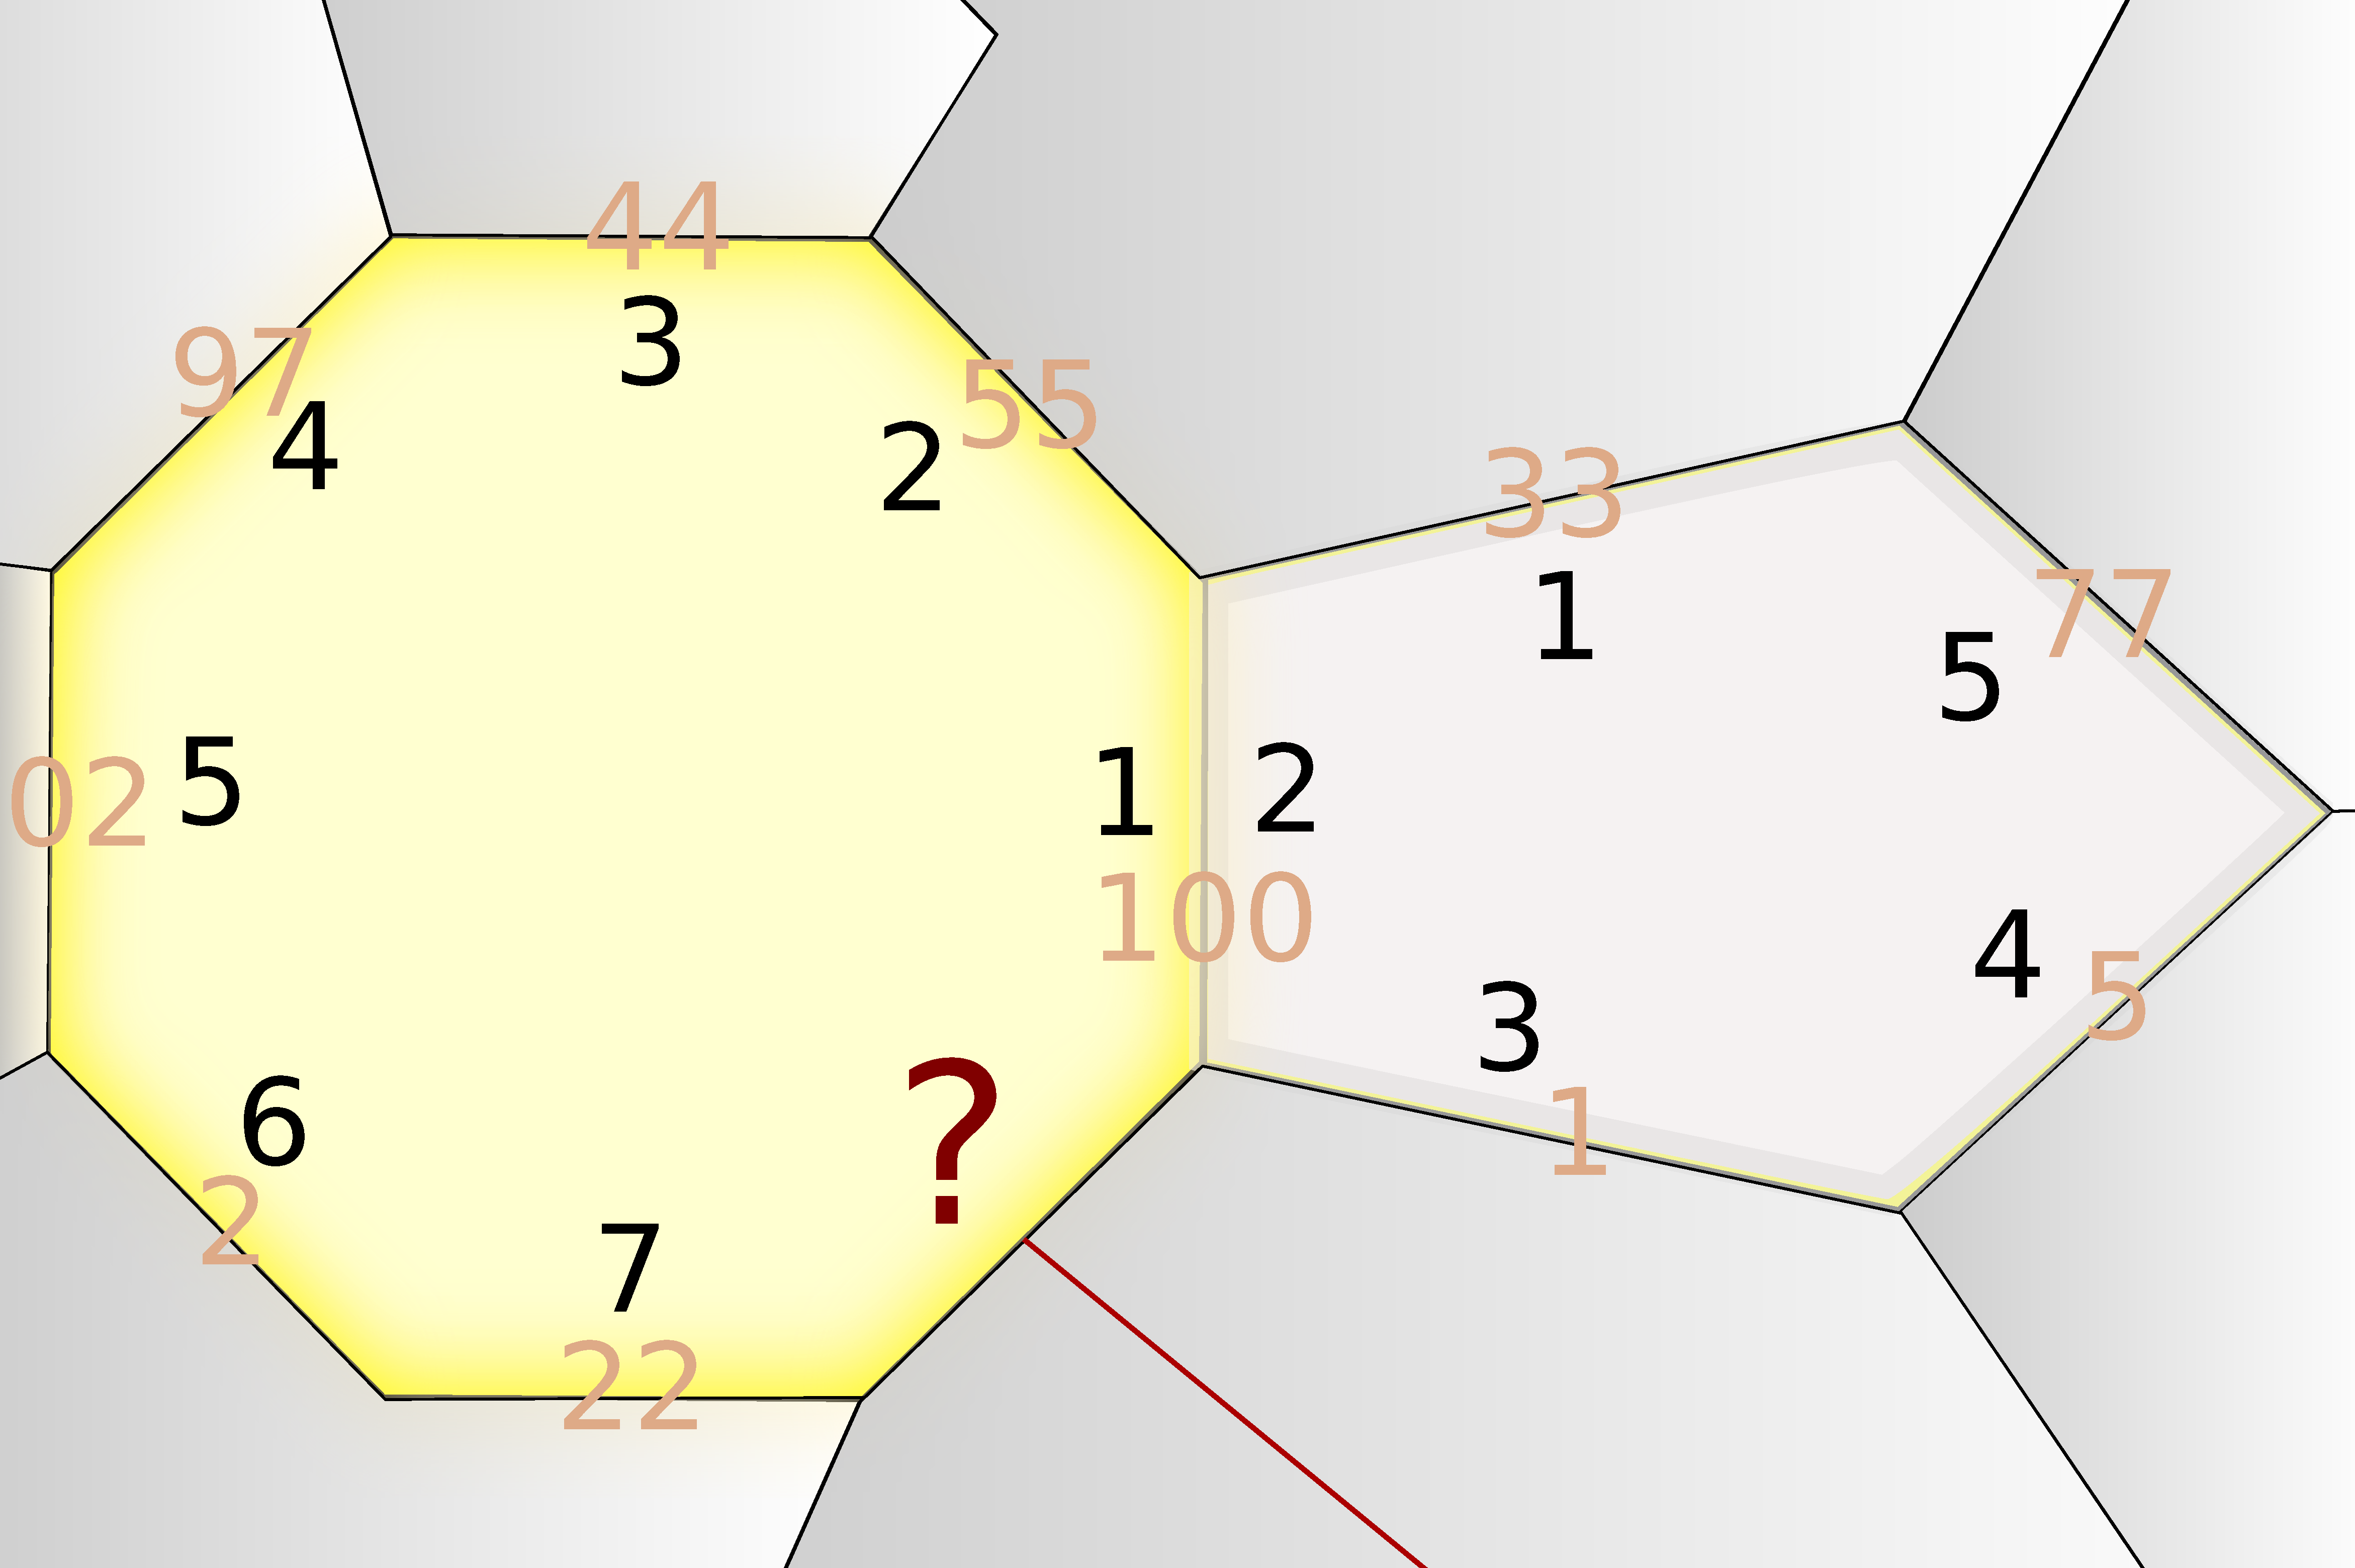
\includegraphics[width=6cm, height=4cm]{img/two_fes_hanging_node_qmark.pdf}}
      } {
        \alt<-2> {\frame{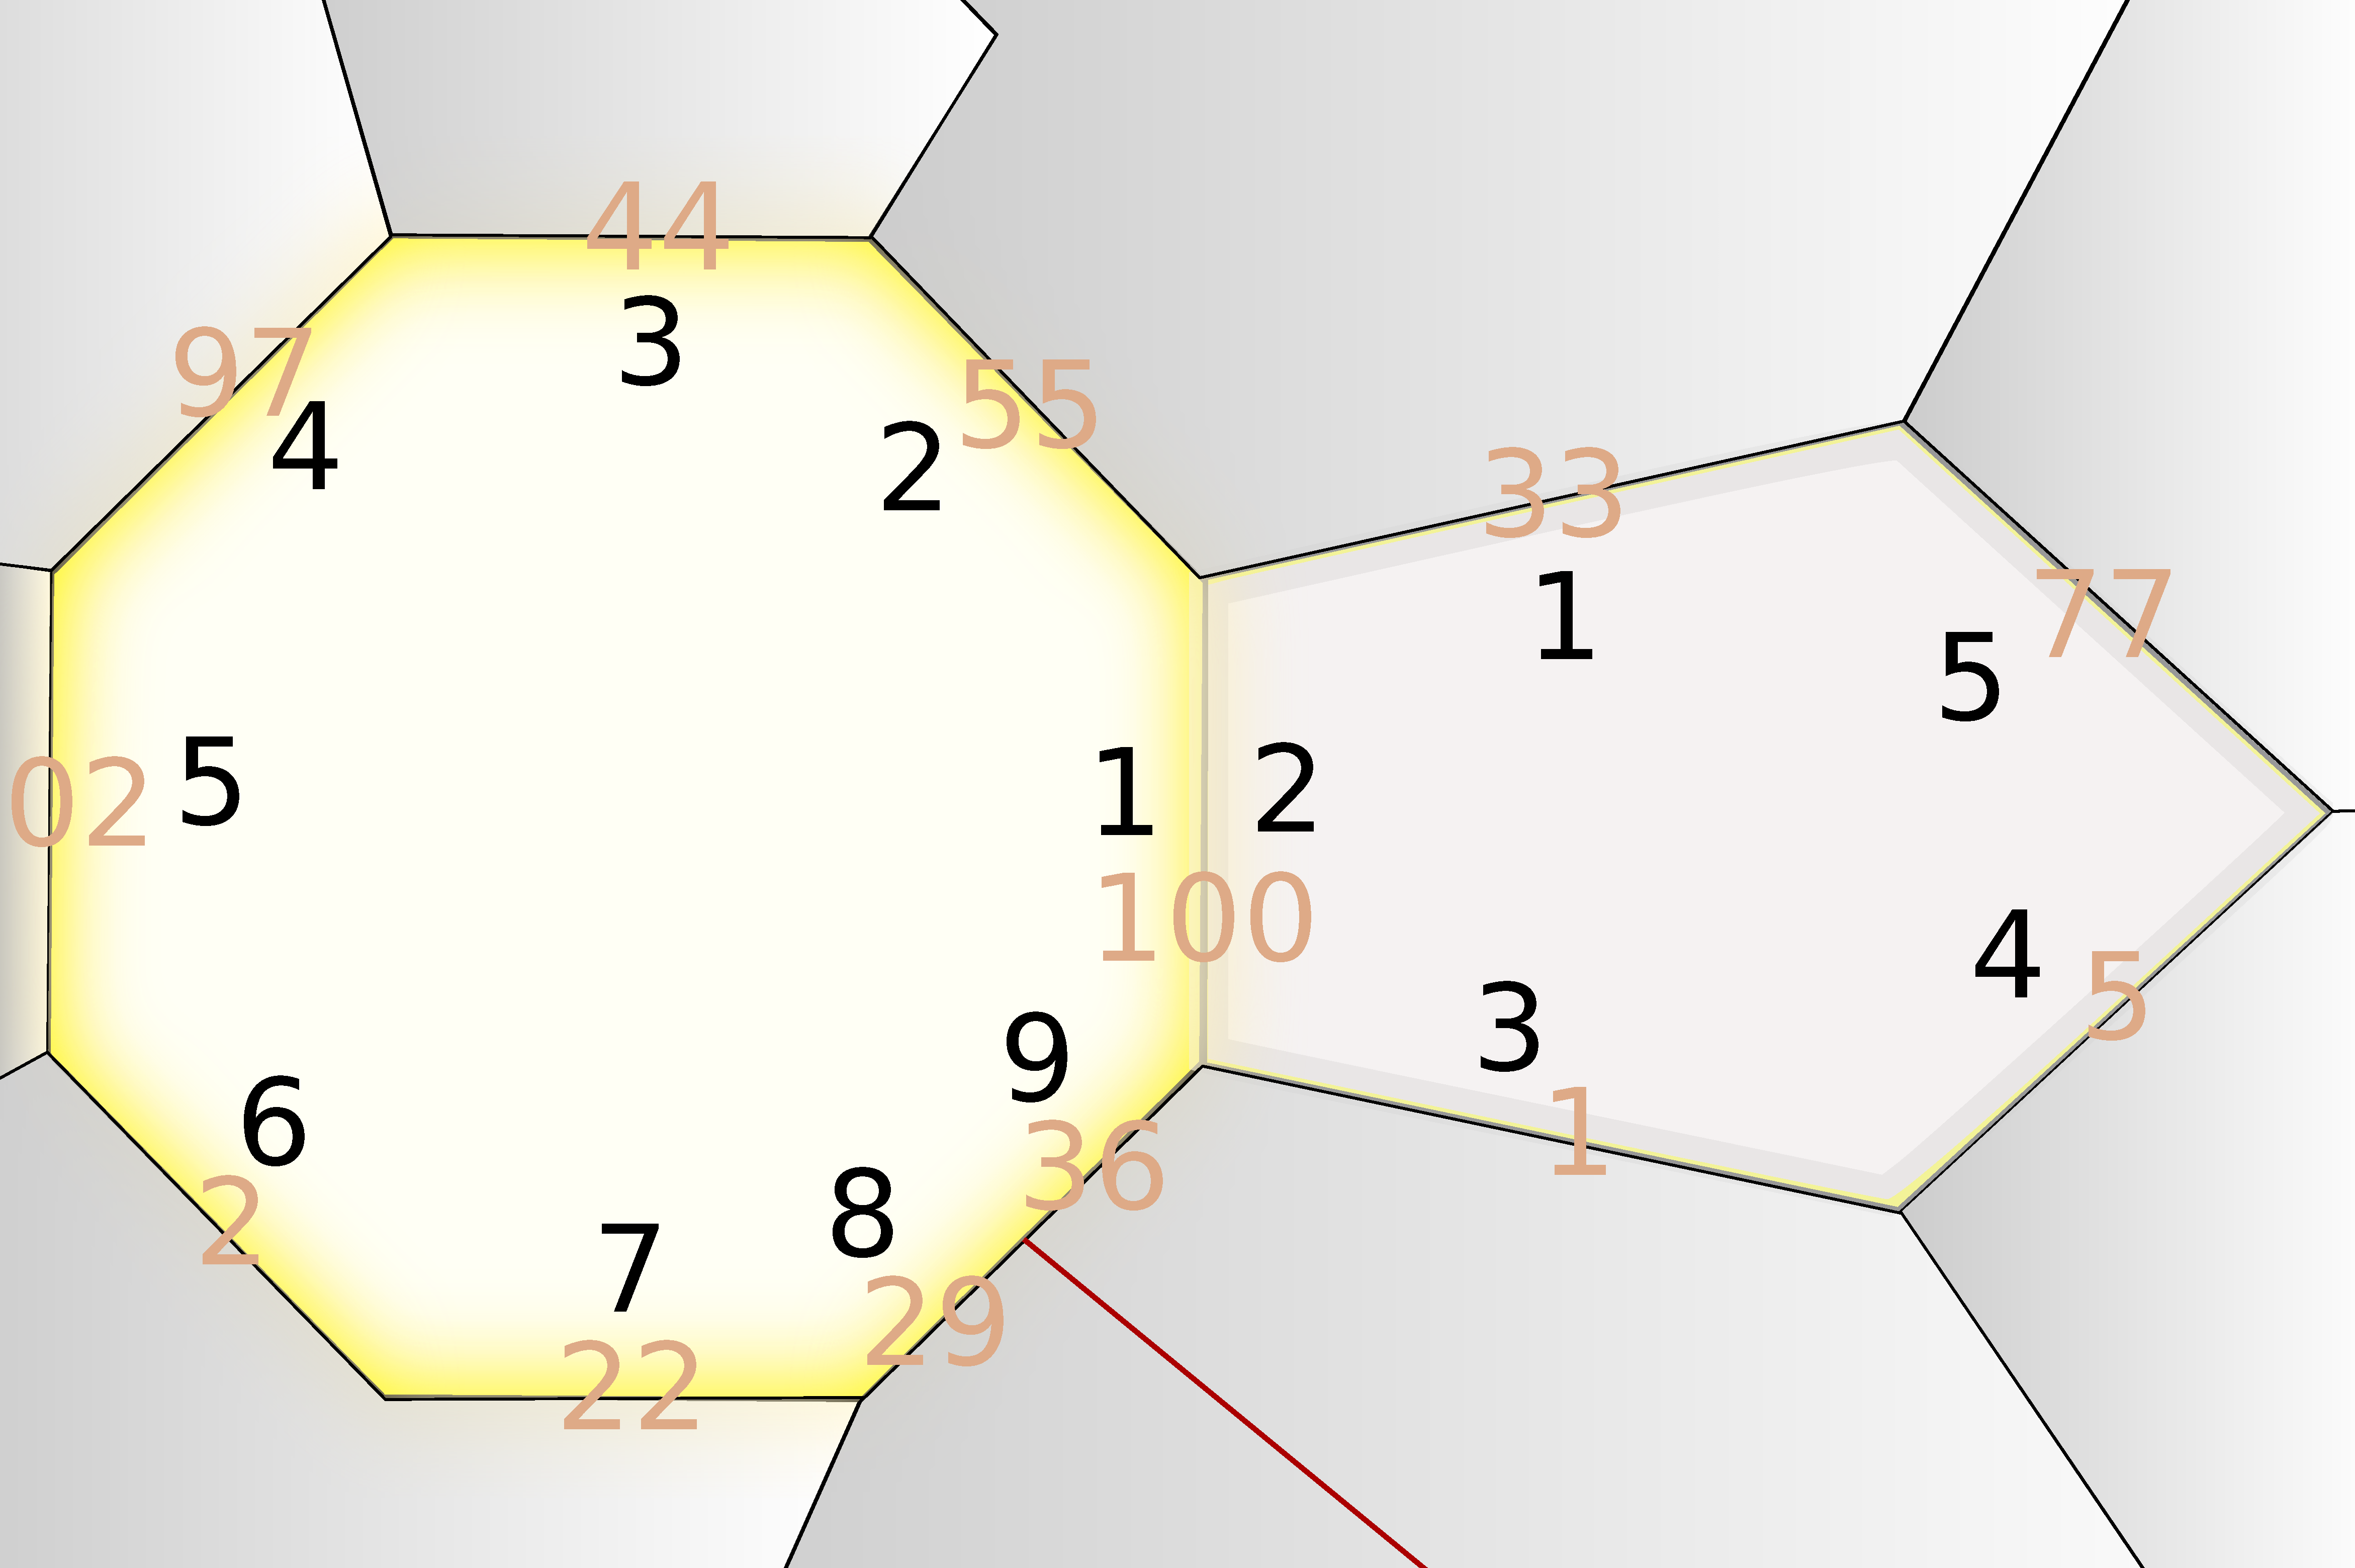
\includegraphics[width=6cm, height=4cm]{img/two_fes_hanging_node_resolved.pdf}}}
                 {\frame{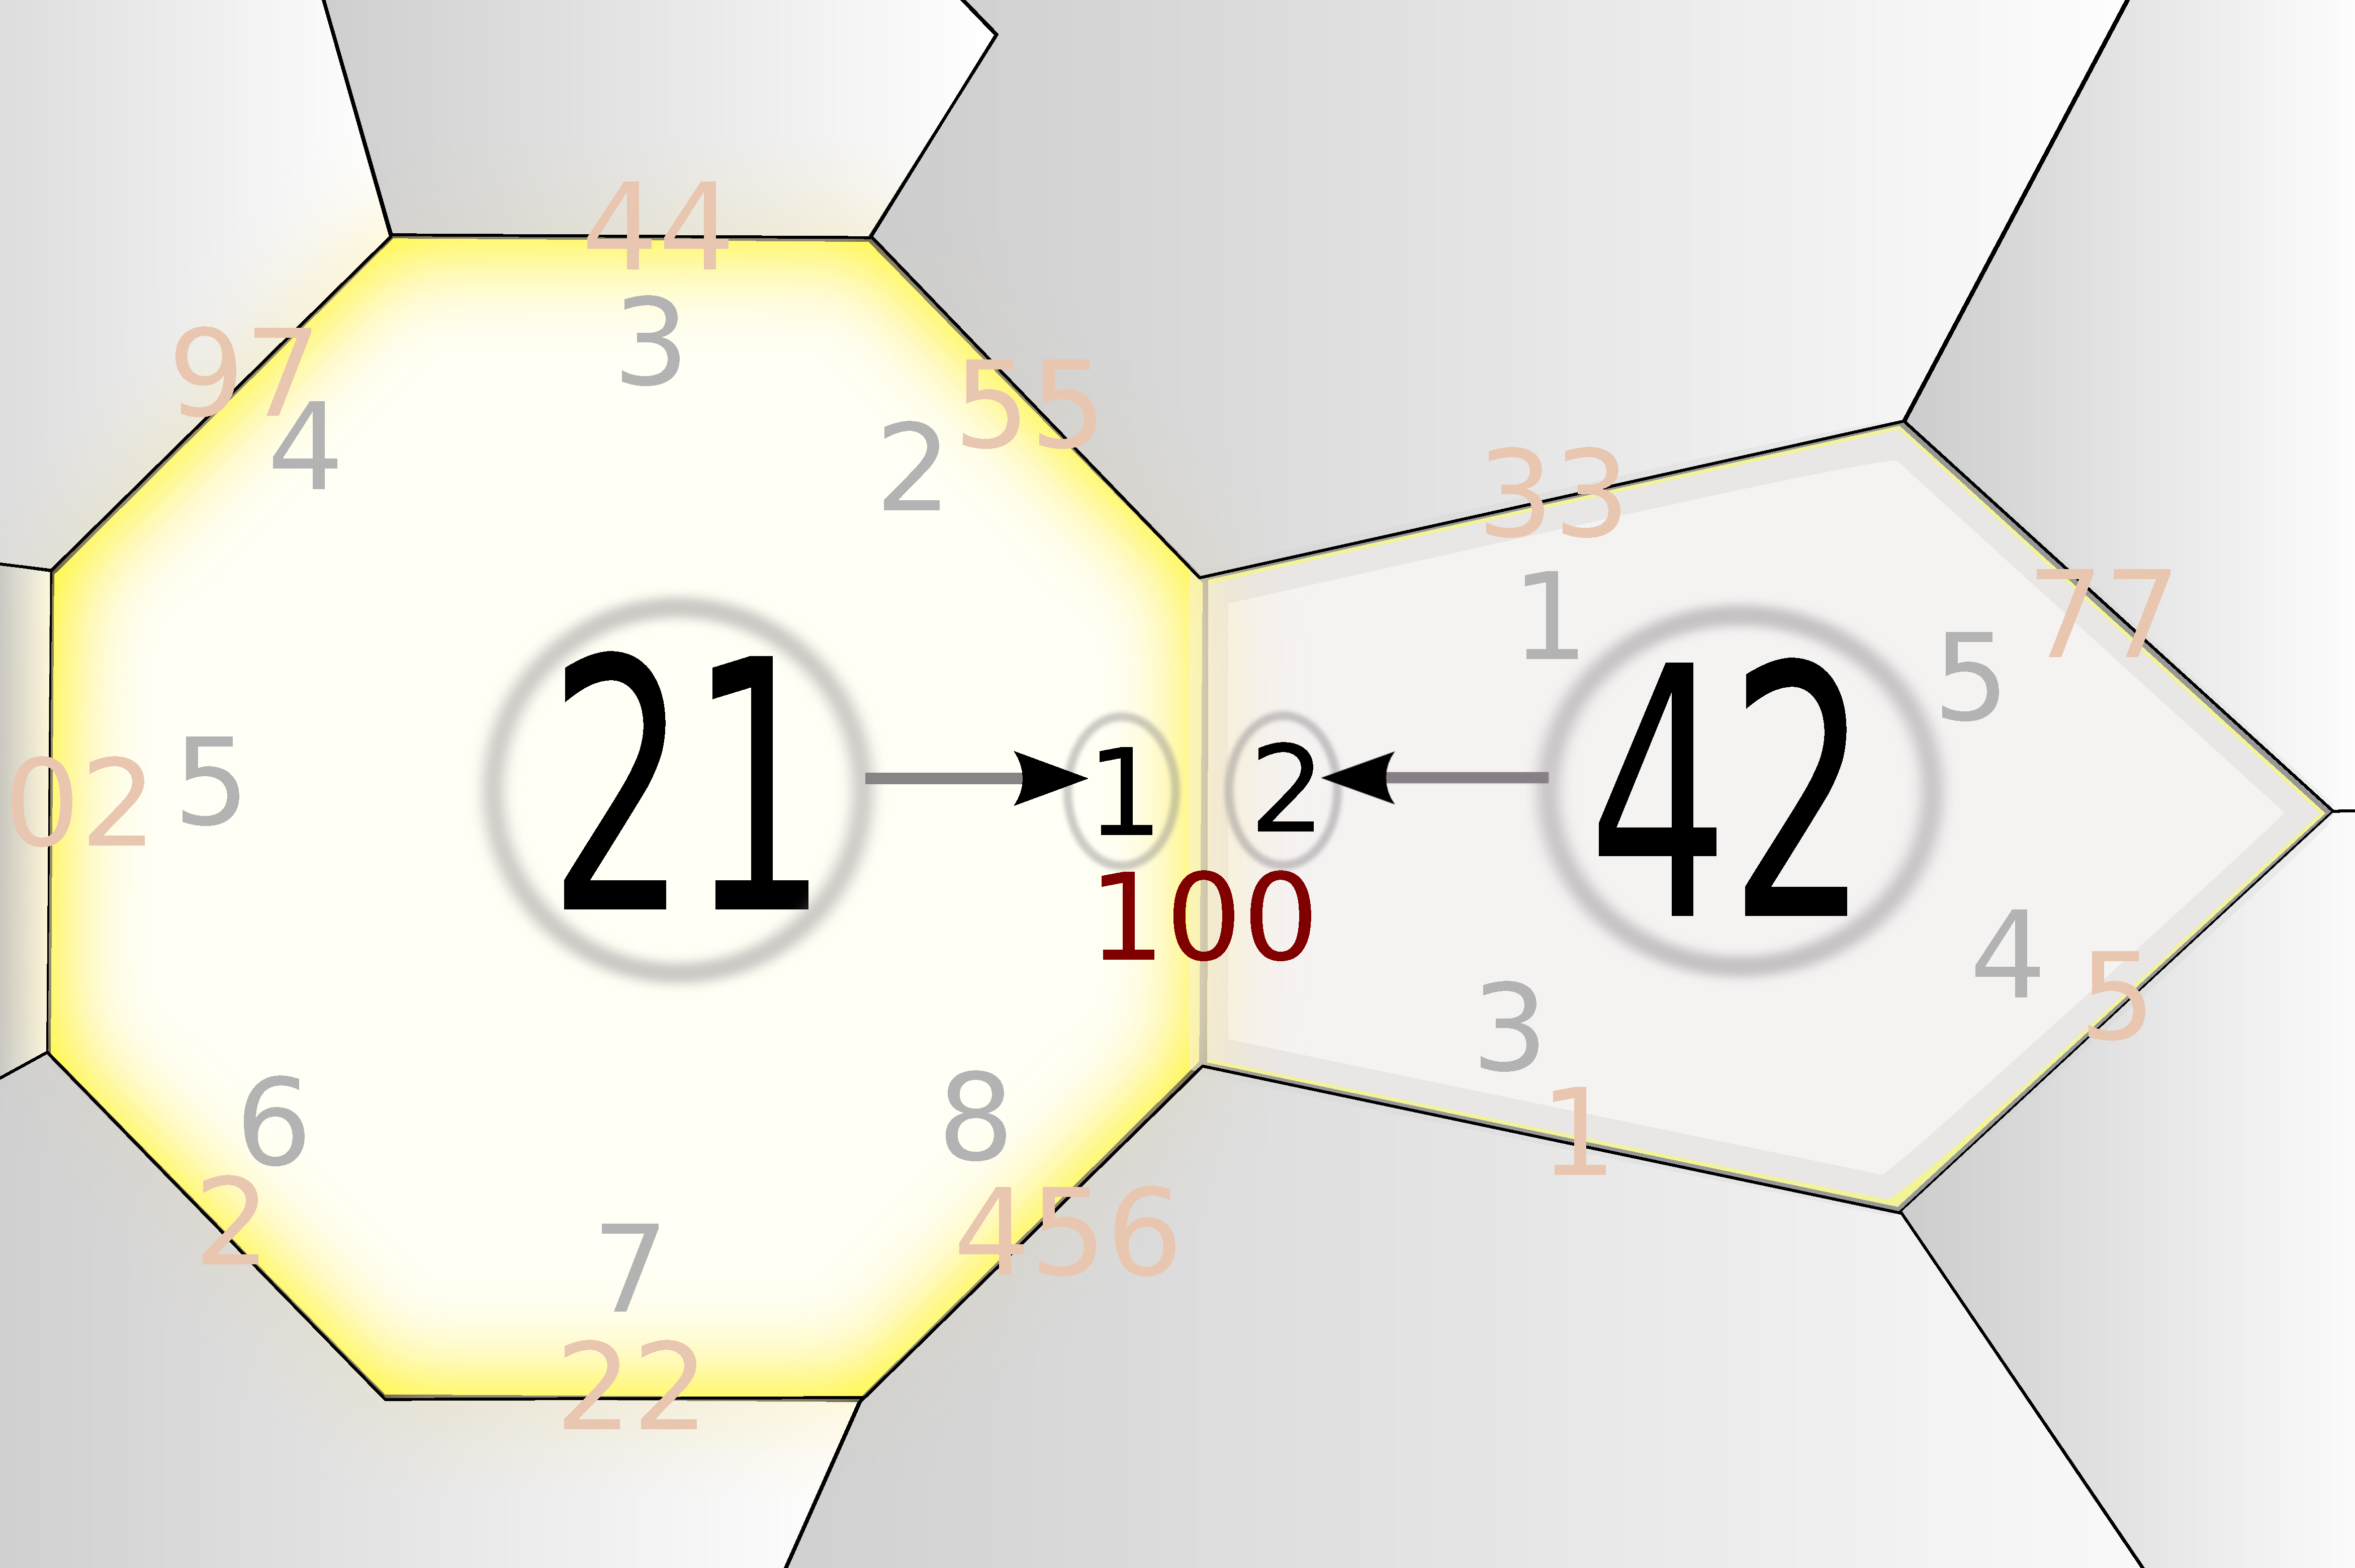
\includegraphics[width=6cm, height=4cm]{img/two_fes_nbsideincls.pdf}}}
      }
  \end{columns}
  \begin{itemize}[<+->]
    \item The \emph{\textbf{finite element inclusions}} of a non-boundary side are the couple of finite elements which include the side,
      each paired with the side face of the side in the including element.
    \item For any non-boundary side, represents the two \emph{\textbf{local representations}} of the side as it occurs in finite elements.
  \end{itemize}
\end{frame}

\subsubsection{Summing Up: Initial Mesh Contract}

\begin{frame}
  \frametitle{Summing Up Mesh Concepts: Initial Mesh Contract}
  \begin{itemize}[<+->]
    \item We can already determine some of the requirements for our abstract mesh contract.
    \item Types \\
      $FENum, NBSideNum, OShape, SideFace = \mathbb{N}$.\\
      $NBSideInclusions = (FENum \times SideFace) \times (FENum \times SideFace)$.
    \item Then the mesh must provide the following functions (incomplete):
      \begin{itemize}[<+->]
        \item \textcolor{blue}{num\_fes}: $() \rightarrow \mathbb{N}$
        \item \textcolor{blue}{num\_nb\_sides:} $() \rightarrow \mathbb{N}$
        \item \textcolor{blue}{num\_oriented\_element\_shapes}: $() \rightarrow \mathbb{N}$
        \item \textcolor{blue}{oriented\_shape\_for\_fe}:  $FENum \rightarrow OShape$
        \item \textcolor{blue}{num\_side\_faces\_for\_shape}: $OShape \rightarrow \mathbb{N}$
        \item \textcolor{blue}{fe\_inclusions\_of\_nb\_side}: $NBSideNum \rightarrow NBSideInclusions $
        \item \textcolor{blue}{nb\_side\_num\_for\_fe\_side}: $FENum \times SideFace \rightarrow NBSideNum$
      \end{itemize}
  \end{itemize}
\end{frame}

\subsection{Approximation space}

\subsubsection{Shape Functions}

\begin{frame}
  \frametitle{WG Shape Functions}
  \begin{itemize}[<+->]
    \item The WG approximation space consists of piecewise polynomials on mesh element interiors and non-boundary sides,
      satisfying degree constraints, and which are 0 on mesh boundary sides.
    \item Interiors and sides may have distinct degree constraints as groups, each limited either by max monomial degree or max variable degree.
    \item As a building block for our basis, we'll define a \emph{\textbf{shape function}} to be a function which is a monomial on one face
      (interior or side) pre-composed with a translation function providing a face-specific origin, which satisfies the appropriate
      degree constraint for the face.
    \item Such shape functions can be chosen to equal any untranslated polynomials of the same degree constraint on their supporting faces,
      which implies that these shape functions taken together \emph{\textbf{span the WG approximation space}}. 
  \end{itemize}
\end{frame}


\subsubsection{Face-Local Origins}

\begin{frame}
  \frametitle{Face-Local Origins for Shape Functions}
  \begin{itemize}[<+->]
    \item Use of face-local coordinates allows many computations involving shape functions to be done only once per oriented shape
      instead of once per finite element, which is crucial for computational efficiency.
    \item To achieve this, face-local origins must be chosen carefully.
    \item A face's local origin should \emph{not} be chosen based on the face's inclusion in a specific element, which would preclude doing
          calculations on oriented shapes as proxies for multiple finite elements.
    \item A side's local origin should \emph{not} be chosen based on the side's membership in an oriented shape, because this representation
      is not unique.
    \item Local origins \emph{\textbf{should}} be based on some \emph{\textbf{translation-independent}}, \emph{\textbf{intrinsic}} geometric
      property of the face. Good choices are the \textbf{centroid}, or the \textbf{vertex of minimum coordinates}.
  \end{itemize}
\end{frame}

\begin{frame}
  \frametitle{Face-Local Origins for Shape Functions (Contd)}
  \begin{columns}
    \column{.50\textwidth}
      \frame{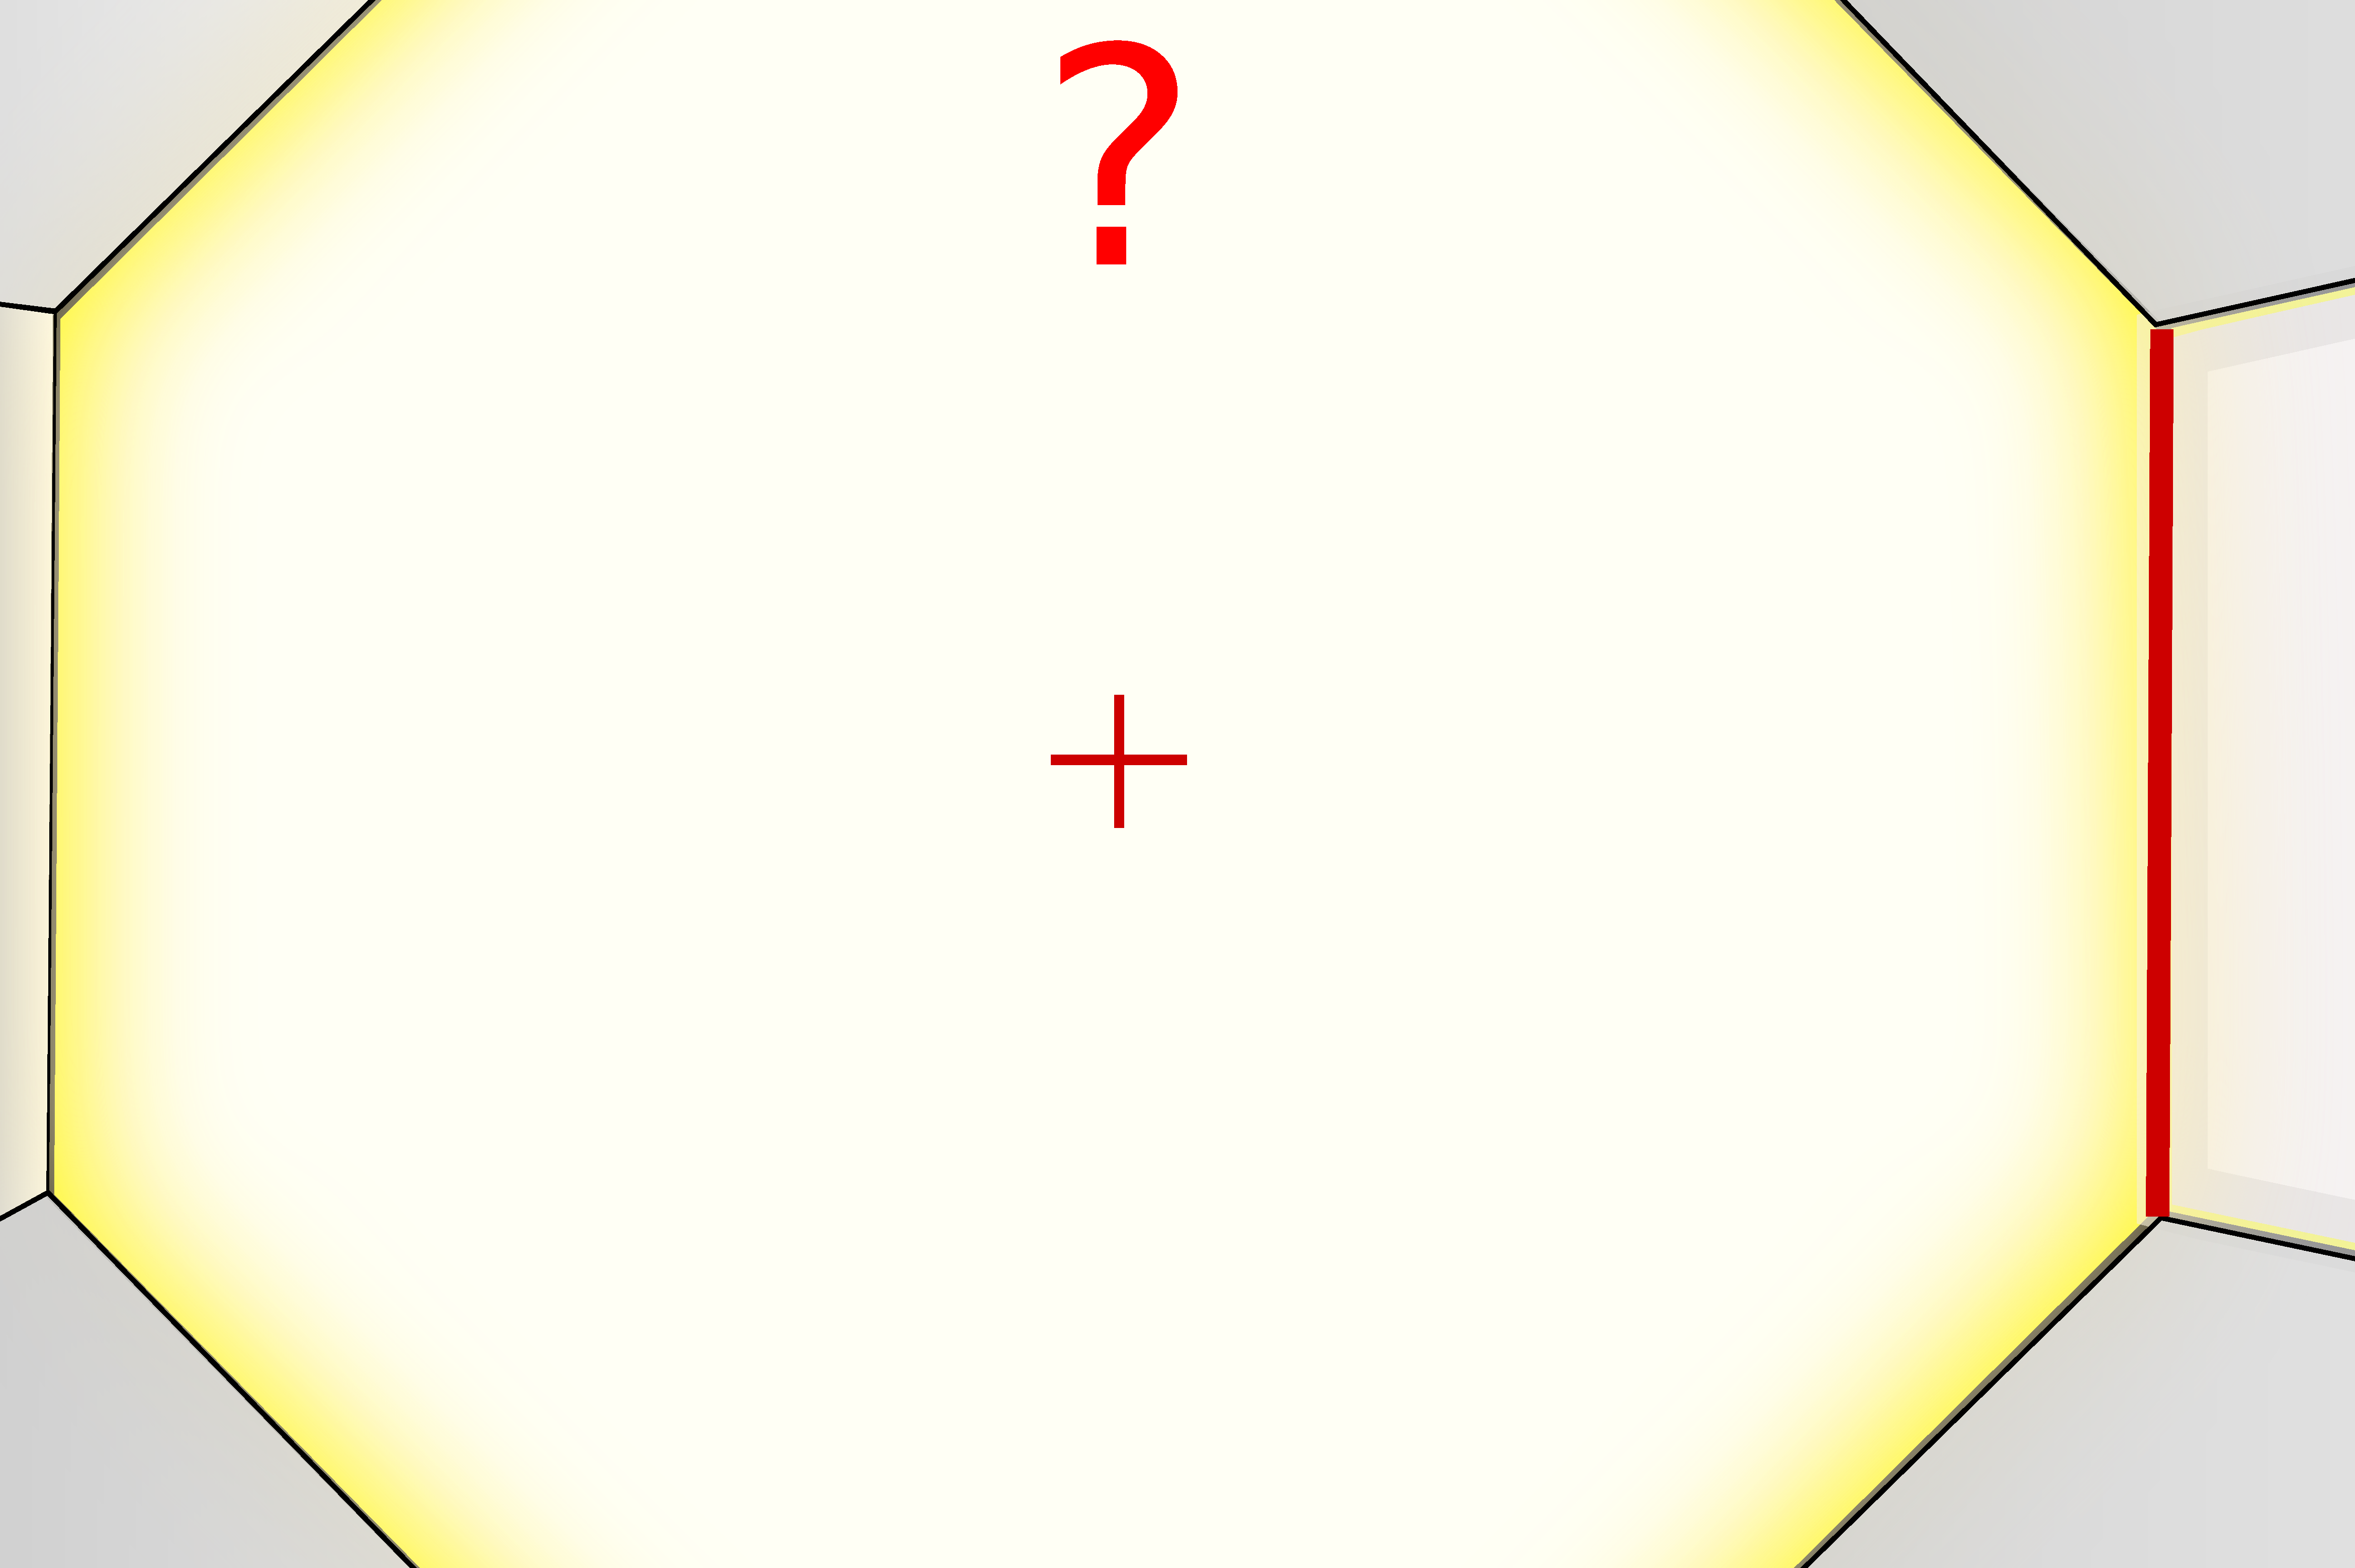
\includegraphics[width=6cm, height=4cm]{img/two_fes_bad_side_origin_1.pdf}}
    \column{.50\textwidth}
      \frame{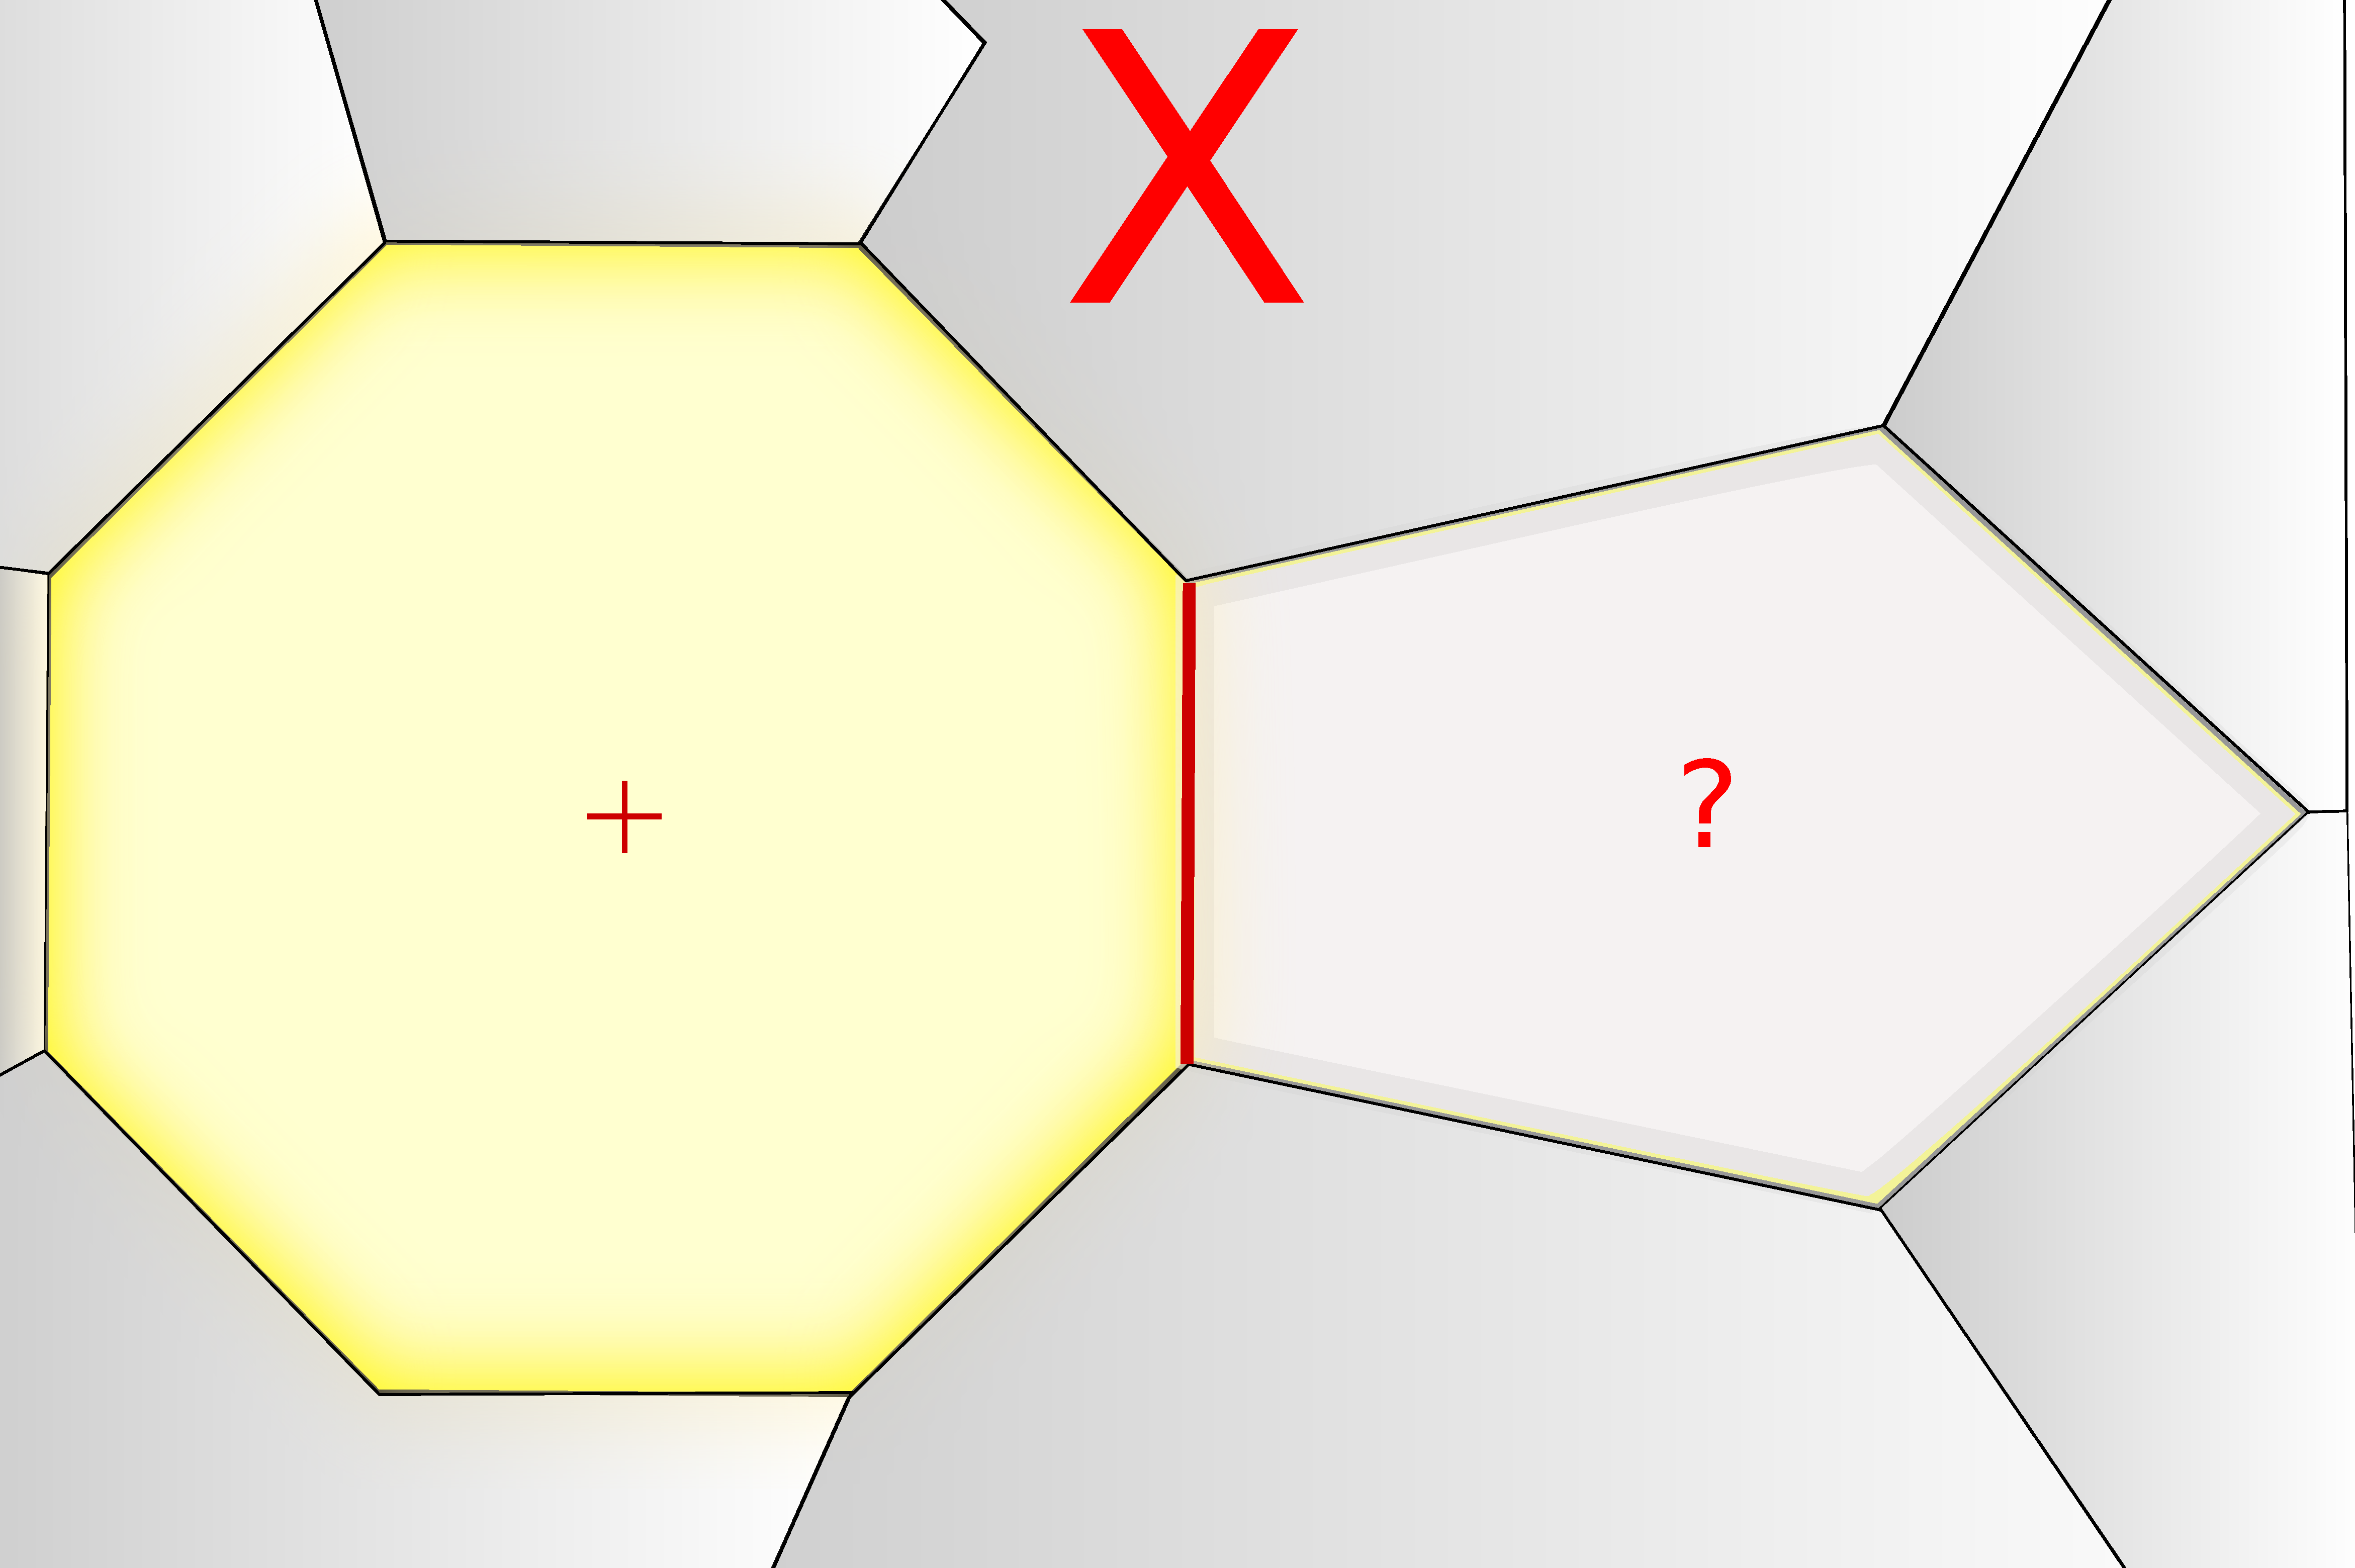
\includegraphics[width=6cm, height=4cm]{img/two_fes_bad_side_origin_2.pdf}}
  \end{columns}
  \begin{itemize}[<+->]
    \item On the left, it is tempting to choose a common origin for the sides and interior of the element, to make calculations easier.
    \item This choice would be difficult to apply consistently, however. A calculation on the right hand element must also use this origin
      for its left side, even if specific elements are not in context such as for calculations on the oriented shape for the right element.
      Rules could be applied in special meshes to achieve this, but they would be ``fragile'' because of the number of assumptions required.
  \end{itemize}
\end{frame}

\subsubsection{Shape Function Independence}

\begin{frame}
  \frametitle{Shape Function Independence}
  \begin{columns}
    \column{.50\textwidth}
      \frame{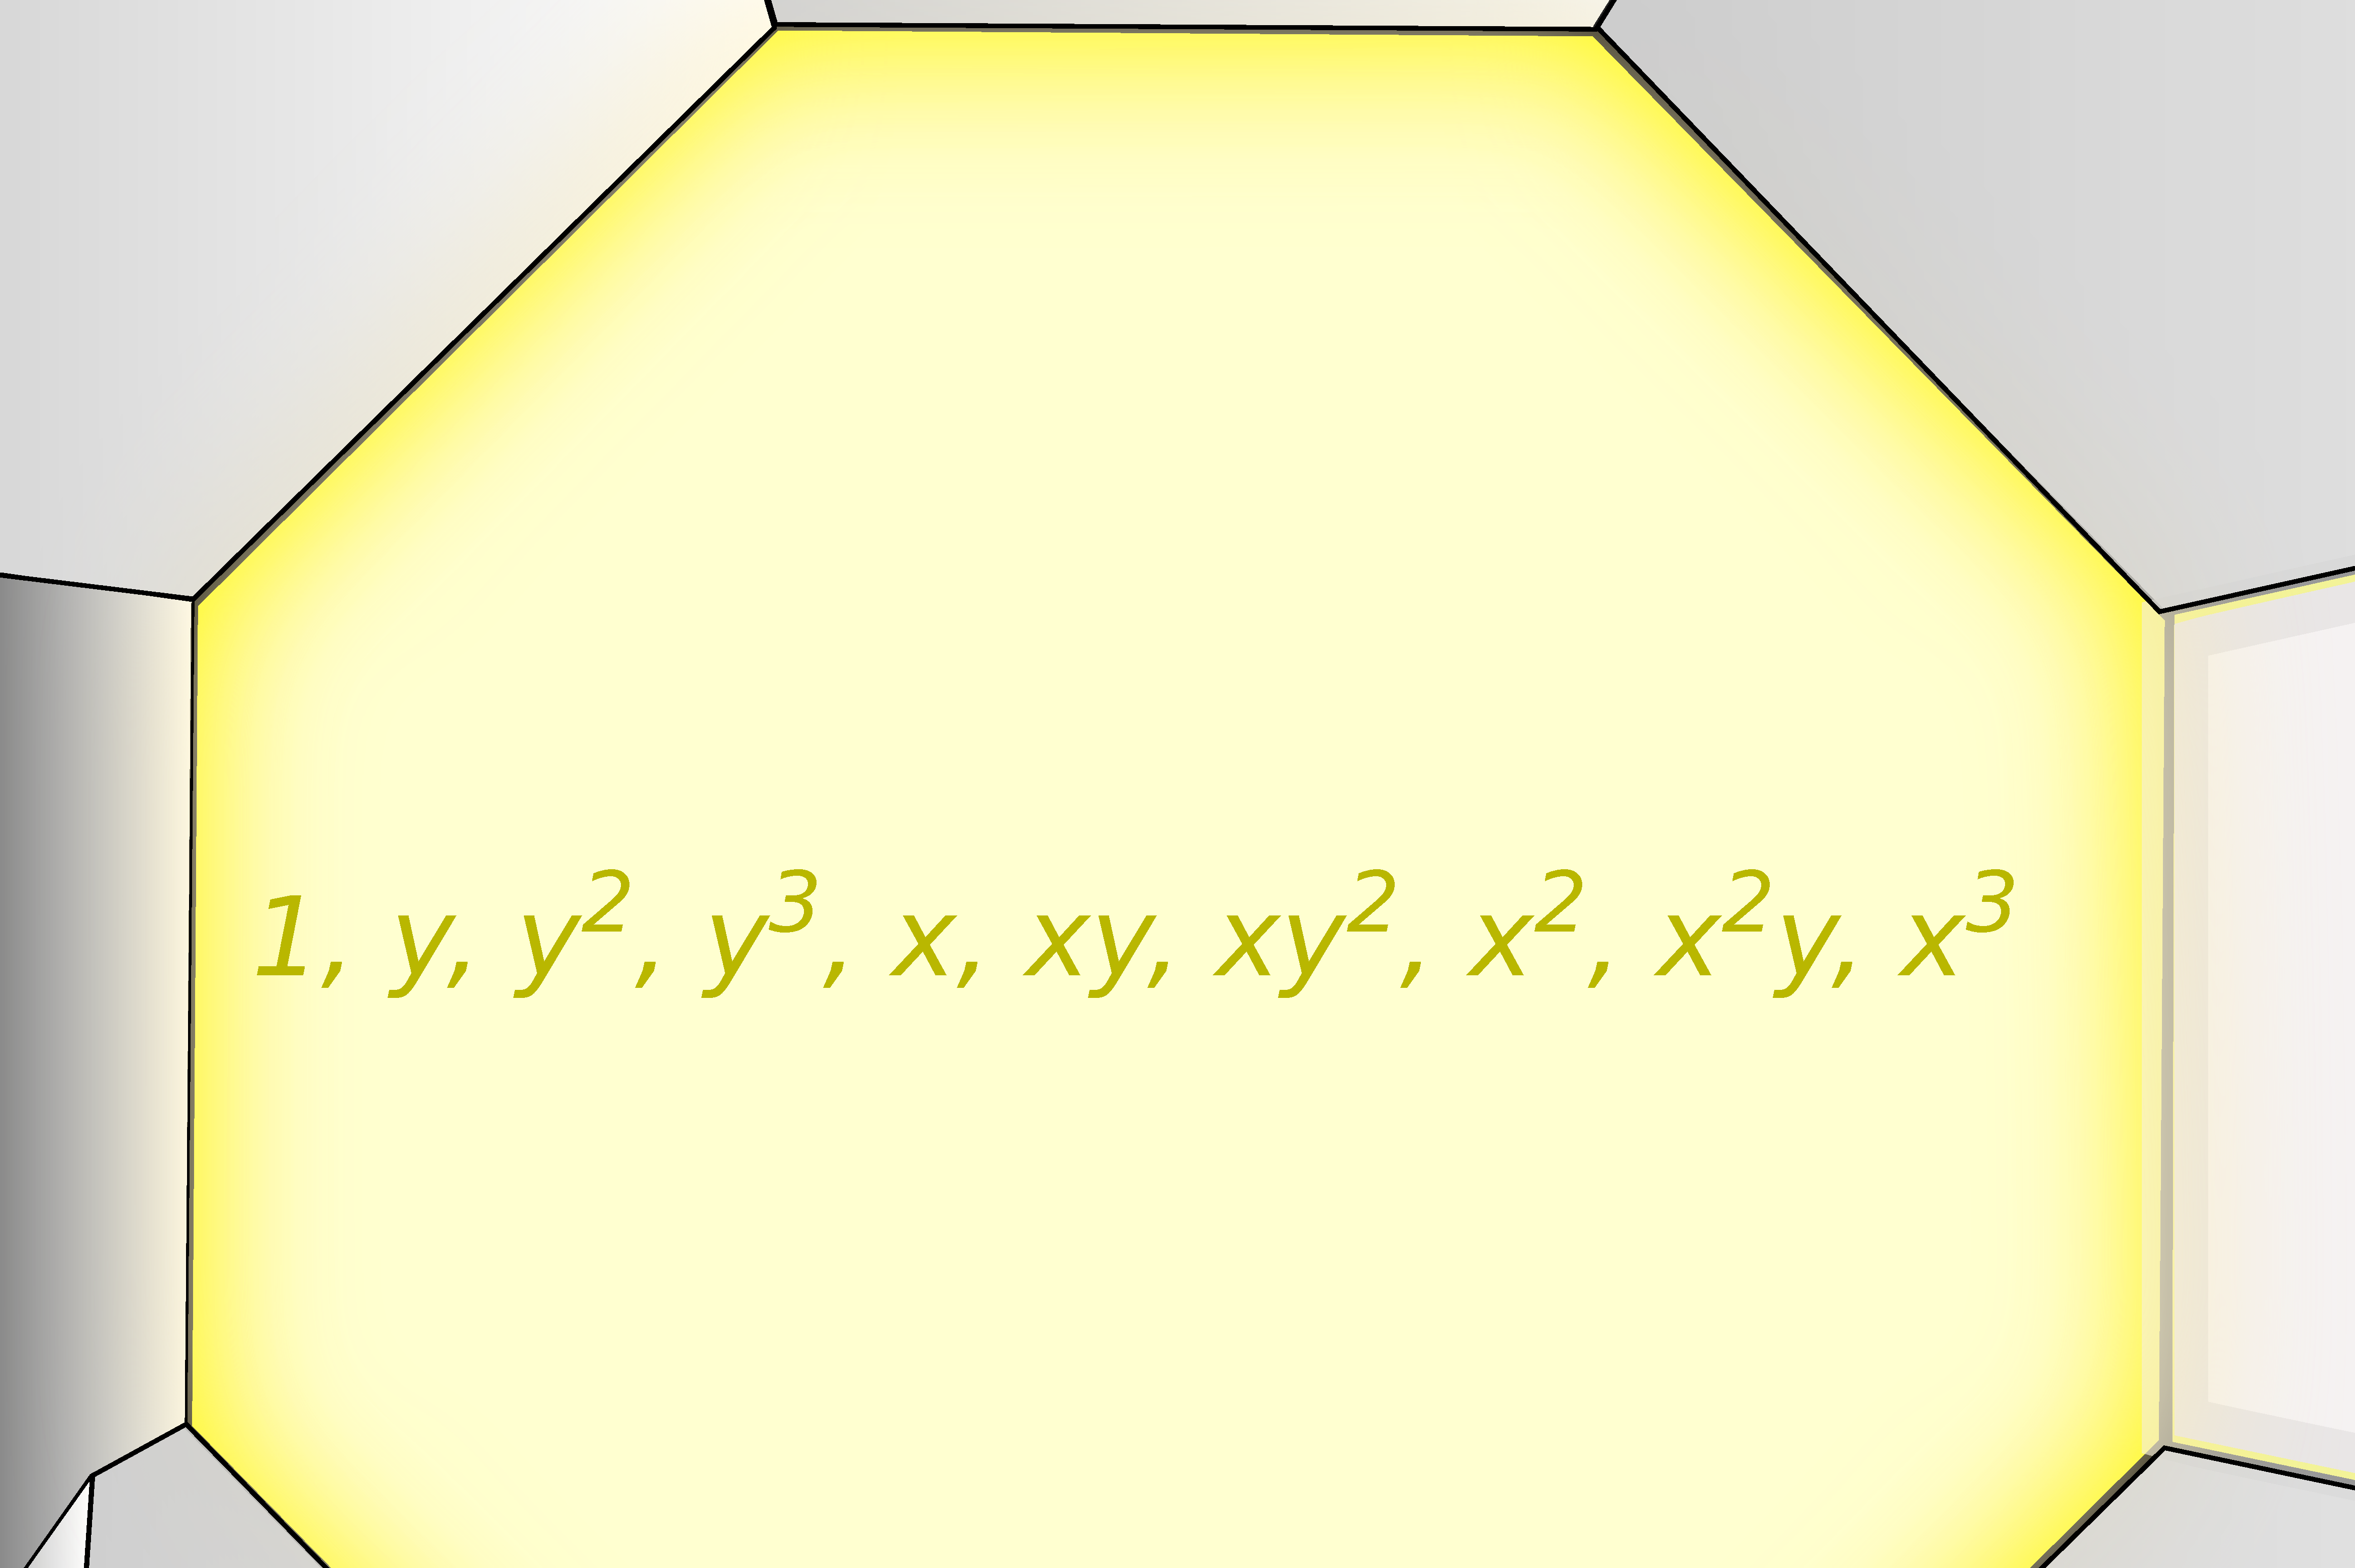
\includegraphics[width=6cm, height=4cm]{img/fe_shapefun_int_mons.pdf}}
    \column{.50\textwidth}
      \pause
      \begin{itemize}[<+->]
        \item Interior supported shape functions are linearly independent, by induction on the space dimension $d$ and
          the fundamental theorem of algebra.
      \end{itemize}
  \end{columns}
  \uncover<+-> {
    \begin{columns}
    \column{.50\textwidth}
    \frame{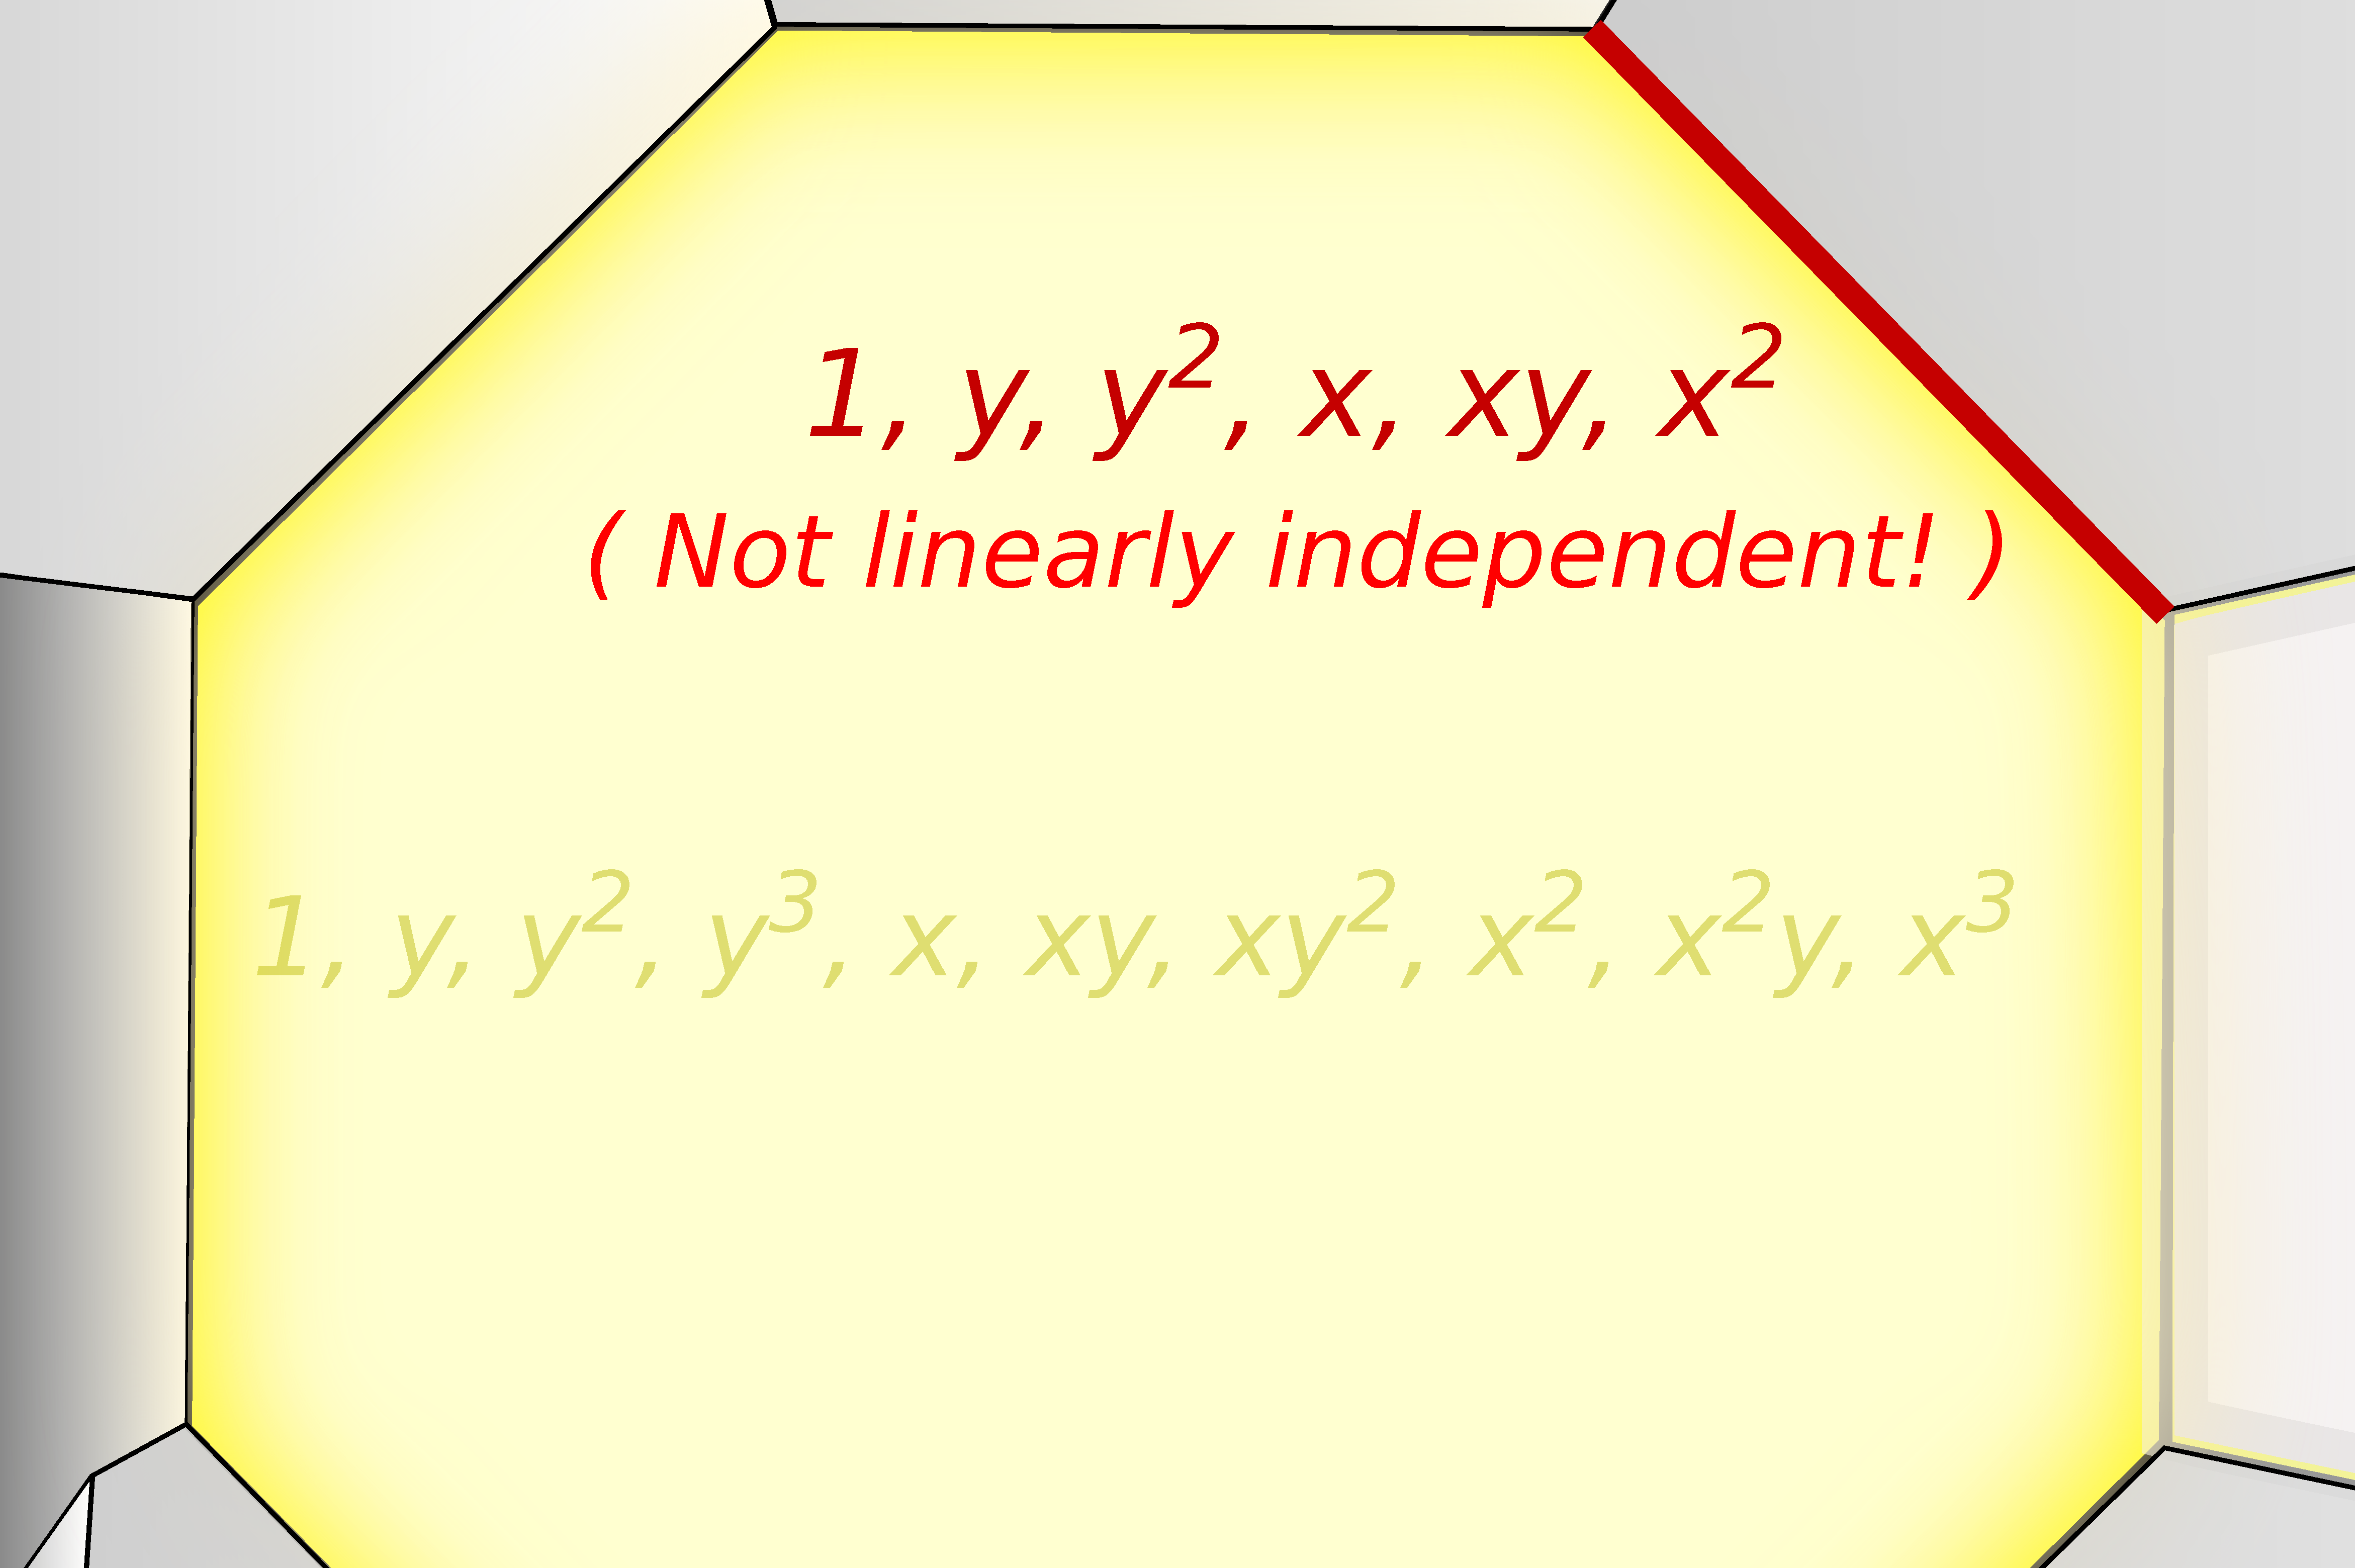
\includegraphics[trim=30pc 40pc 0cm 0cm, clip=true, width=6cm, height=3.4cm]{img/fe_shapefun_side_mons_int_greyed.pdf}}
    \column{.50\textwidth}
      \begin{itemize}[<+->]
        \item However the full set of side supported shape functions are \emph{\textbf{linearly dependent}}. E.g. $y=-x$ for all $(x,y)$ on the side pictured,
          so that $y^2=x^2$, $x y = -x^2$, etc.,  on the side.
      \end{itemize}
    \end{columns}
  }
\end{frame}

\subsubsection{Side Dependent Dimension}

\begin{frame}
  \frametitle{Side Dependent Dimension}
  \begin{itemize}[<+->]
  \item The subset of shape functions supported on a side which are linearly independent depends on the side's orientation.
  \item Each side has at least one \emph{\textbf{dependent dimension}}, which is a space dimension which can be written as an affine
      function of the others on the side, as expressed in the side's local coordinate system.
  \end{itemize}
  \uncover<+-> {
    \begin{block}{Existence of Dependent Dimension for a Side}
      We take as given that a side is a translated subset of a subspace $S$ of dimension $d-1$ of $\mathbb{R}^d$. Then $S$ is the solution
      of a single linear equation, $S = \left\{(x_1,\dots,x_d): \sum_{i} a_i x_i = 0\right\}, \text{where some } a_j \ne 0$,
        so that $x_j$ is a linear combination of the other $x_i$ on $S$. This holds for coordinates relative to an origin within $S$.
        If the side's origin is outside the side, then recasting to that origin yields an affine function.
    \end{block}
  }
\end{frame}

\begin{frame}
  \frametitle{Side Dependent Dimensions Illustrated}
    \frame{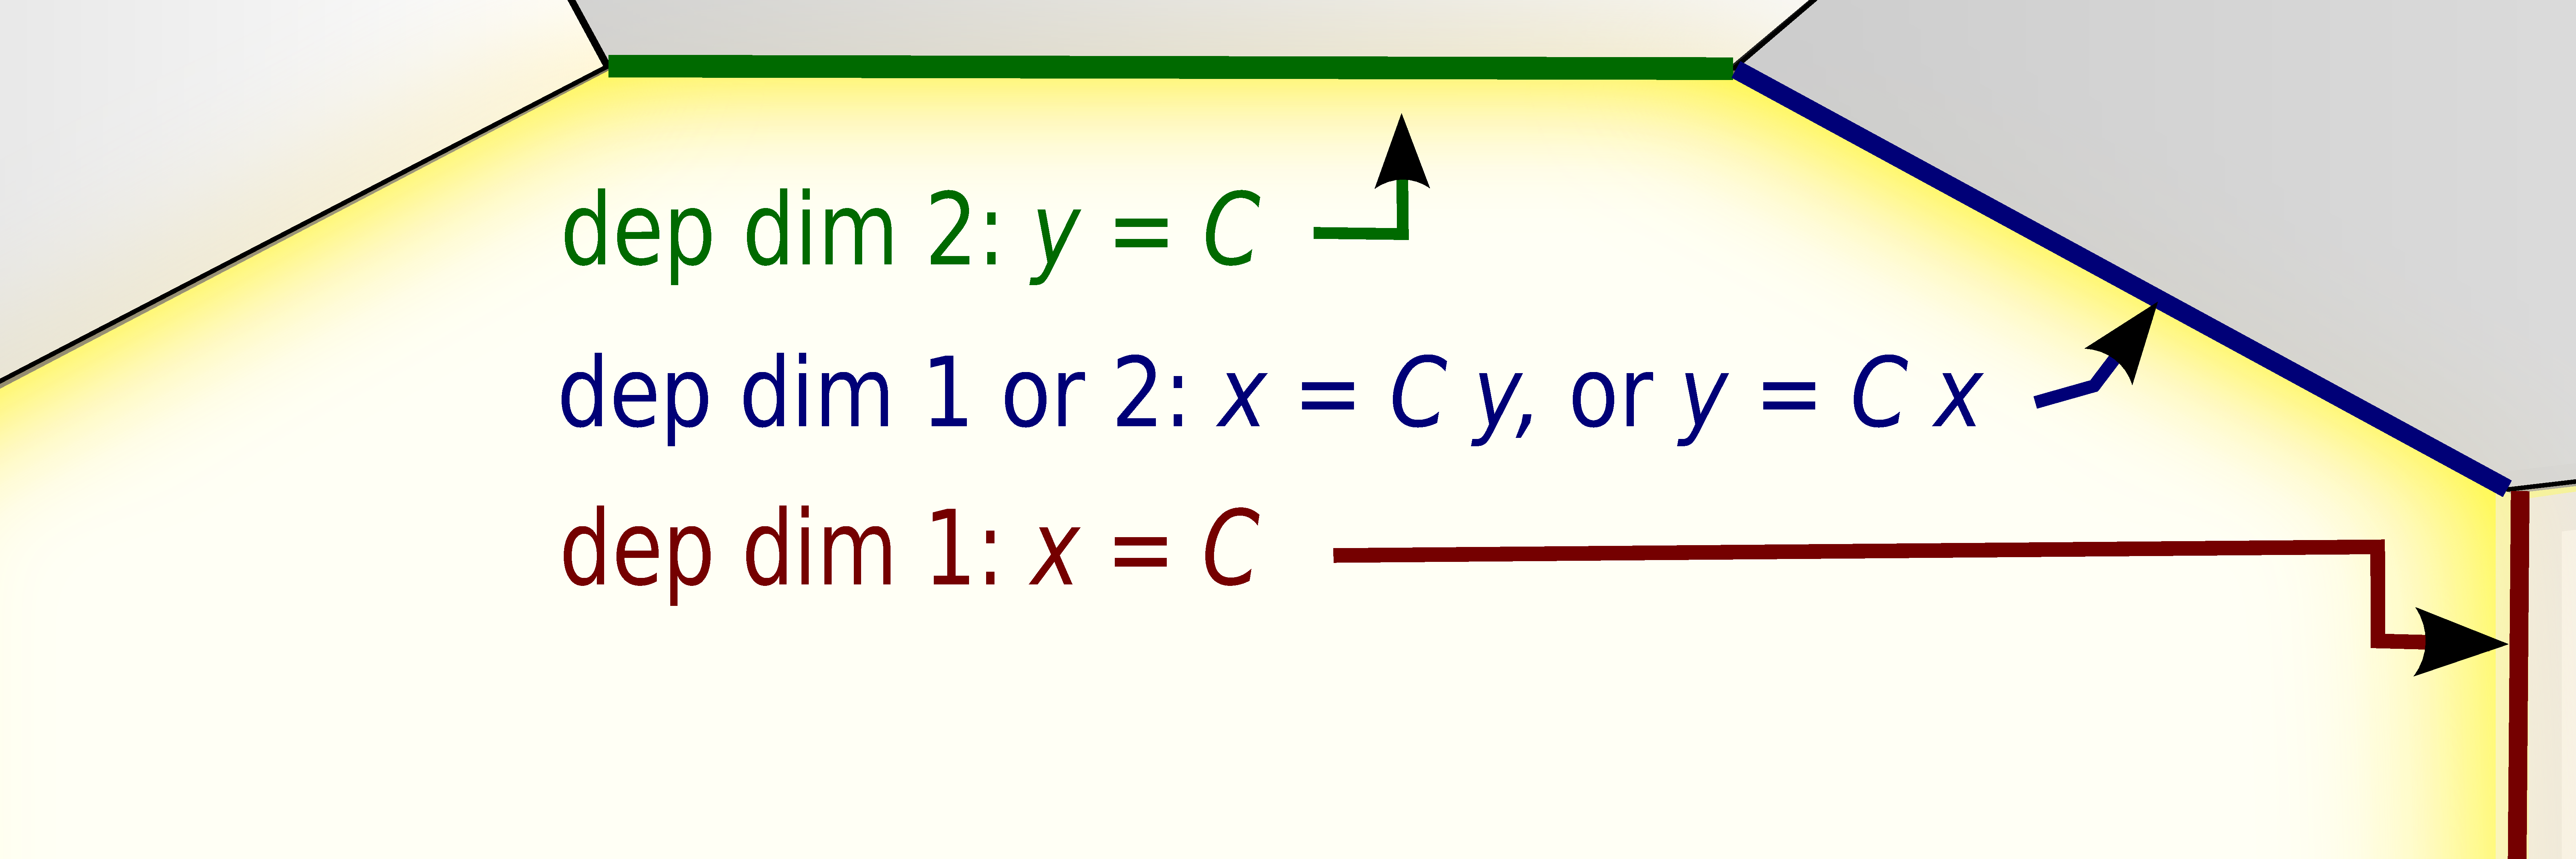
\includegraphics[width=12cm, height=4cm]{img/side_dep_dims_2d.pdf}}
    \begin{itemize}[<+->]
      \item Dependent dimensions must be chosen by the mesh for \emph{each} side, so the basis can choose shape functions to support on the sides.
        Thus to the mesh contract we we add a new function,
        {\small \texttt{\textcolor{blue}{mesh.\textbf{\textcolor{orange}{dependent\_dim\_for\_oshape\_side}(oshape, sf)}}}}.
      \item Choice should be based on intrinsic geometric properties of the side, not its representation in finite elements
        (which precludes oshape ops) or in oriented shapes (representation not unique).
    \end{itemize}
\end{frame}


\begin{frame}
  \frametitle{Side Dependent Dimension -- Contd}
  \begin{itemize}[<+->]
    \item To form a linearly independent set of shape functions supported on a side, we will \emph{\textbf{omit the shape functions
      having any non-zero power of the dependent dimension variable}}.
    \item The reduced set of shape functions spans the same space as the full set, because with a dependent of dimension $j$,
      any monomial of the full set can be expressed as
       $$x_1^{k_1} \dots x_j^{k_j} \dots x_d^{k_d}
           \;\; = \;\; x_1^{k_1} \dots (a_0 + \sum_{i \ne j} a_i x_{i})^{k_j} \dots x_d^{k_d}\text{,}$$
      which expands to a polynomial which is free of $x_j$. Additionally, the right side's maximum monomial degree will not exceed
      that of the left.  For constraints on the maximum variable degree, if $a_i = 0$ for $i \ge 1$,
      as is the case with rectangle meshes, then we again have the right hand side satisfying any max variable degree constraint
      that the left side does. In either case, the original monomial has been expressed as a linear combination of monomials in the reduced set.
    \item TODO: Proof of independence.
  \end{itemize}
\end{frame}


\begin{frame}
  \frametitle{Side Dependent Dimension -- What Do I Do?}
  \pause
  Start with all monomials satisfying side degree constraints, e.g. to degree $k-1$, then drop some monomials as follows:
  \pause
  \frame{
\includegraphics[width=12cm, height=2.59cm]{img/side_dep_dims_visual_summary_2d.pdf}}
  \pause
  \frame{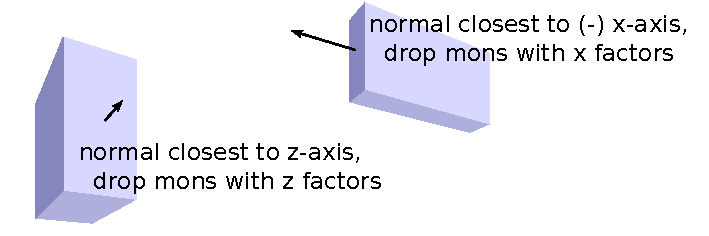
\includegraphics[width=12cm, height=4cm]{img/side_dep_dims_visual_summary_3d.pdf}}
\end{frame}


\subsection{Variational Bilinear Form}

\subsubsection{Practicality of Computation}

\begin{frame}
  \frametitle{Variational Bilinear Form - Practicality}
  $$\spot<1->{\mathfrak{a}}(u_h,v) = (f,v)\quad\quad \forall{v} \in V_{h0}$$
  \begin{itemize}[<+->]
    \item Some additional requirements on the vbf are necessary for computations to be feasible at even moderate scale.
    \item For example for $k=3$ and a 50x50 mesh, there are already 39,700 basis elements, and \emph{1,576,090,000} 
      \emph{interactions} between elements. 
    \item The majority of these interactions will yield $0$ vbf value, but we need to avoid computing as many as possible.
    \item We'll use two additional requirements on the vbf to eliminate many unnecessary calculations:
        \begin{itemize}[<+->]
          \item \emph{\textbf{Element summability}} and associated \emph{\textbf{locality}} property, allowing element-wise operations and
            forbidding ``action at a distance''
          \item a \emph{\textbf{translation invariance}} property, allowing calculations to be done on a general oriented shape in place of
            calculations on individual finite elements of the shape
        \end{itemize}
    \item Requirements are aligned with general spirit of FEM's.
  \end{itemize}
\end{frame}

\begin{frame}
  \frametitle{Example Variational Bilinear Form}
  $$\mathfrak a_s(v,w) = \sum_{T \in M} \left\{ (a \nabla_w v,\nabla_w w)_{\scriptscriptstyle T_0} \;+\;
    h_T^{-1}\langle Q_b v_{\scriptscriptstyle T_0} - v,Q_b w_{\scriptscriptstyle T_0} - w \rangle_{\partial T} \right\}$$
  \pause
  \begin{itemize}[<+->]
    \item $\mathfrak a_s$ is a sum of contributions from the behavior of the input functions considered
      separately on individual finite elements.
    \item When computing the contribution from a given element, values of the input functions outside the element cannot effect the
      element's contribution.
    \item The contribution does not depend on the location of the element:  If we were to ``move'' the input functions by
      pre-composing with a translation, and move the element in the same way, we would obtain the same contribution.
    \item The per-element contribution function is itself a bilinear function of the input functions over the element.
  \end{itemize}
\end{frame}

\subsubsection{Element Summability}

\begin{frame}
  \frametitle{Variational Bilinear Form -- Element Summability}
  \begin{block}{Element Summability}
    The vbf is the sum of contributions of a fixed \emph{local} bilinear form applied over individual elements
    \begin{center}$\mathfrak{a}(v,w) = \sum_T { \phi(v|_T,w|_T) }$\end{center}
      where $u$ and $v$ are piecewise polynomials on the mesh, and $\phi$ is a bilinear form which is independent of the mesh elements $T$.
  \end{block}
  \pause
  \begin{itemize}[<+->]
    \item This allows us to compute element-at-a-time with the vbf.
    \item It implies the \emph{\textbf{locality property}} -- that if there is no finite element that intersects the supports of \emph{both}
      of $v$ and $w$, then $\mathfrak{a}(v,w) = 0$.
        \footnote{We'll also assume that $\phi$ is not sensitive to differences in the functions on sets of no measure in $\mathbb{R}^{d-1}$,
                  so that an element containing only a lesser edge (e.g. vertex) of the support of $u$ or $v$ can be ignored.}
      This greatly reduces the possible non-null interactions between basis elements under the vbf.
  \end{itemize}
\end{frame}

\subsubsection{Translation Invariance}

\begin{frame}
  \frametitle{Variational Bilinear Form -- Translation Invariance}
  \begin{block}{Translation Invariance}
  The local bilinear form $\phi$ is translatable between elements of the same oriented shape, in the following sense.\\
  If $u, v: T_1 \rightarrow \mathbb{R}$ are piecewise polynomials defined on finite element $T_1$, then
    $$\phi(u, v) = \phi(u \circ \tau, v \circ \tau)$$
      whenever $\tau: T_2 \rightarrow T_1$ is a translation to element $T_1$ from an element $T_2$ having
      the same oriented shape as $T_1$.
  \end{block}
  \pause
  \begin{itemize}[<+->]
    \item This allows us to compute vbf values on an oriented shape, in place of computations on individual finite elements.
  \end{itemize}
\end{frame}

\section{Implementation}

\subsection{The Basis}

\subsubsection{Responsibilities}

\begin{frame}
  \frametitle{The Basis -- Responsibilities}
  \begin{columns}
    \column{.65\textwidth}
      \frame{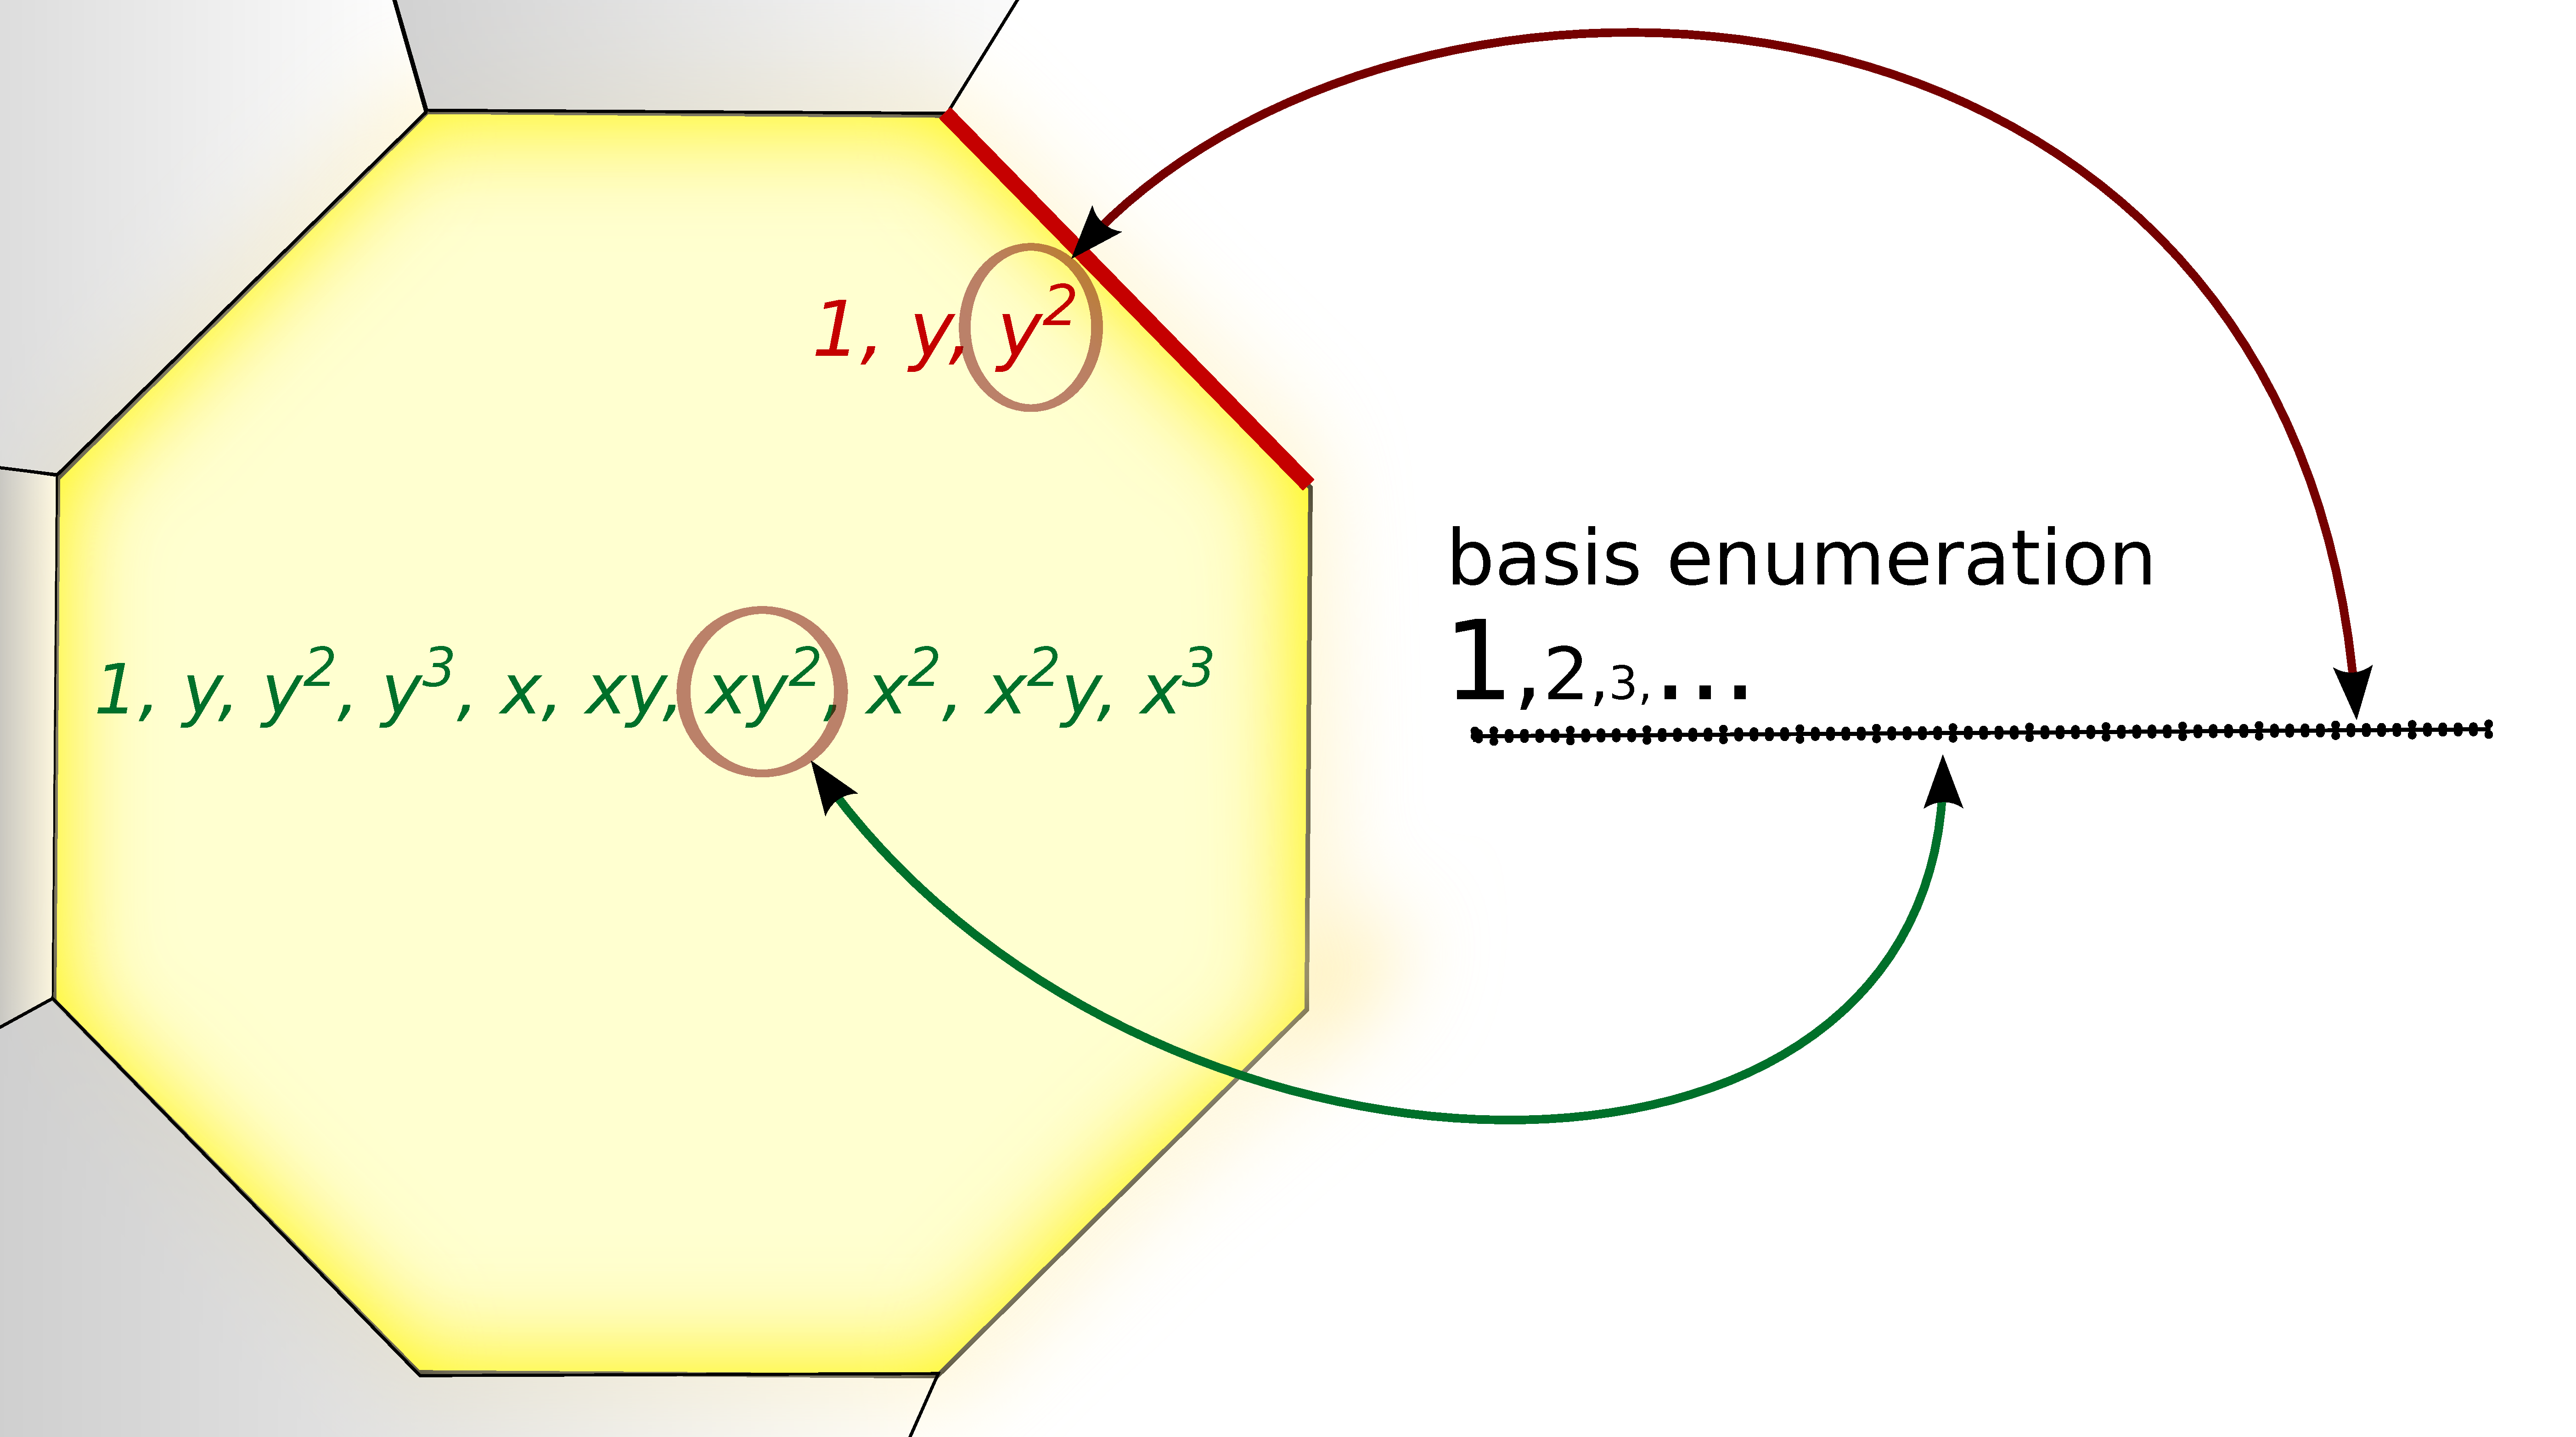
\includegraphics[width=7.16cm, height=4cm]{img/basis_local_global_mapping.pdf}}
    \column{.35\textwidth}
    The main job of the basis module is to translate back and forth between a flat, \emph{\textbf{global}} enumeration
    of all basis elements, and \emph{\textbf{local}} basis element representations suitable for computation.
  \end{columns}
  \pause
  \begin{block}{Basis Element Local Representation}
    A local representation of a basis element is the combination of:
    \begin{itemize}[<+->]
      \item a finite element
      \item the relative face in the finite element on which the basis element is supported: either the interior or relative side face
      \item a monomial or face-relative monomial number
    \end{itemize}
  \end{block}
\end{frame}

\subsubsection{Enumeration Method}

\begin{frame}
  \frametitle{The Basis -- Enumeration Method}
  Basis elements are arranged with interior-supported elements first, followed by those on non-boundary sides.
  The mesh provides relevant counts and any needed information such as side dependent dimensions.
  \frame{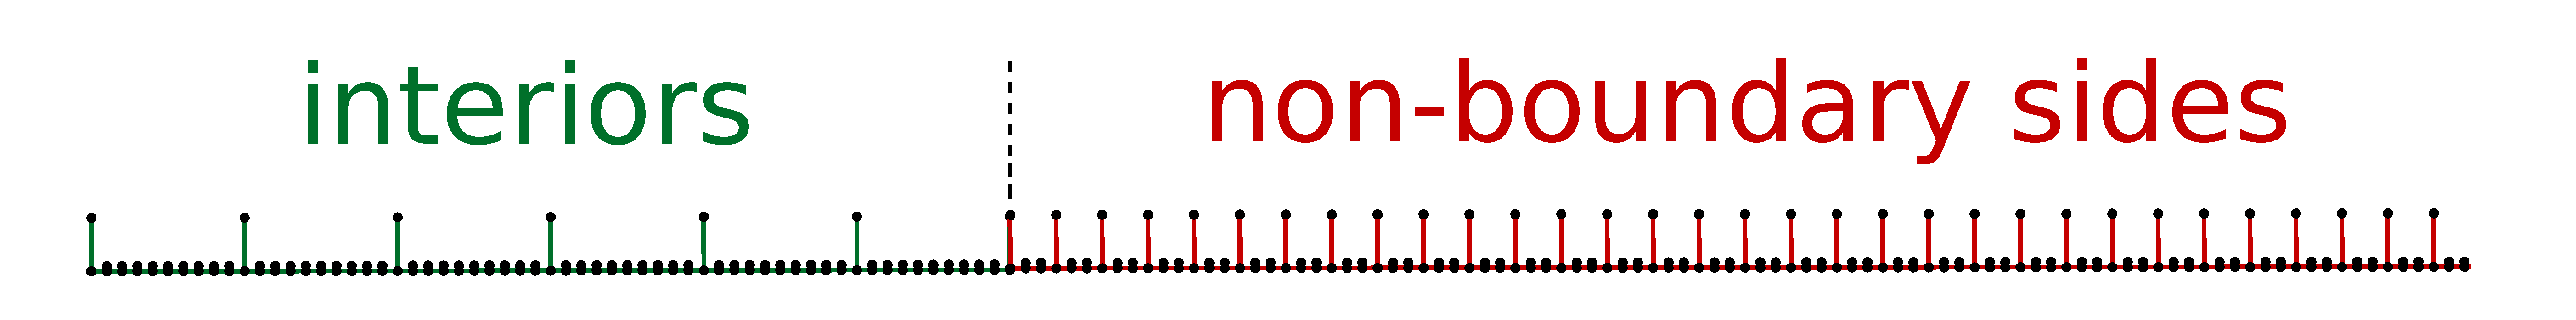
\includegraphics[width=12cm, height=1.49cm]{img/basis_layout_overall.pdf}}
  \pause
  \frame{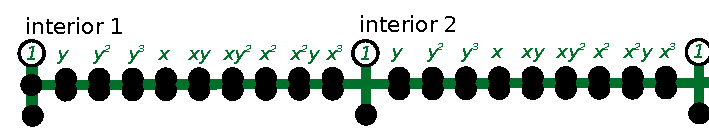
\includegraphics[width=12cm, height=2.2cm]{img/basis_layout_ints.pdf}}
  \pause
  \frame{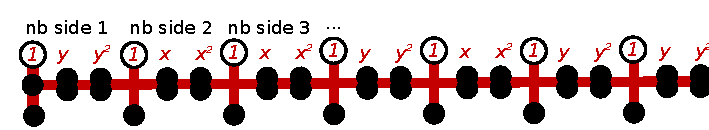
\includegraphics[width=12cm, height=2.2cm]{img/basis_layout_nbsides.pdf}}
\end{frame}

\subsubsection{Implementing Basis Methods}

\begin{frame}
  \frametitle{Implementing the Basis -- Face Monomials}
  \frame{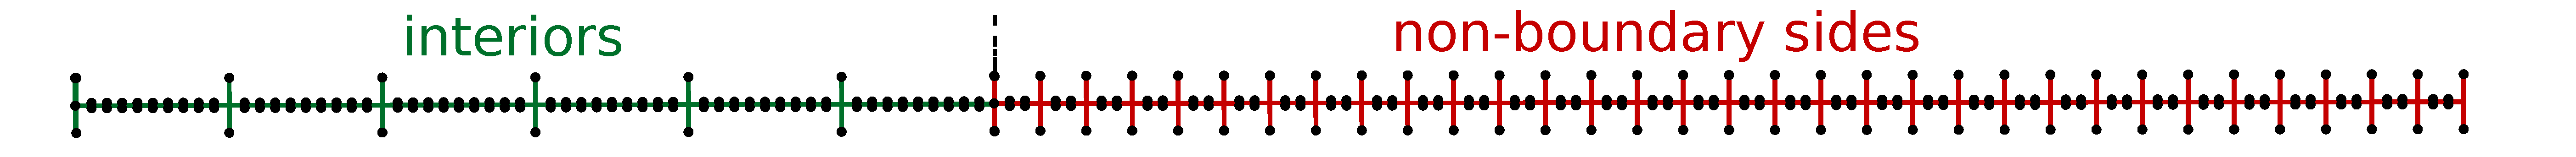
\includegraphics[width=12cm, height=.73cm]{img/basis_layout_overall_thin.pdf}}
      \texttt{\textcolor{blue}{ref\_int\_mons()}},\\ 
      \texttt{\textcolor{blue}{side\_mons\_for\_fe\_side(fe, side\_face)}}, \\
      \texttt{\textcolor{blue}{side\_mons\_for\_oshape\_side(oshape, side\_face)}}\\
      \small
      \begin{itemize}[<+->]
      \item
      When a basis object is being constructed, we create and store in the new object the reference sequence of
      monomials supported on any one interior. We also store reference side monomials, but since these sequences
      vary by side orientation, we create one such sequence for each possible dependent dimension (i.e. for each space dim).
      These functions return those stored sequences. The first function just returns the interior sequence directly.
      \item 
      For the last two functions, we need to find the side's dependent dimension to lookup the proper monomials sequence.
      For the first of the two, we find the oriented shape via 
        {\scriptsize \texttt{\textcolor{blue}{mesh.\textbf{\textcolor{orange}{oriented\_shape\_for\_fe}(fe)}}}}, 
      then defer to the last function.  For the latter, obtain the side dependent dimension via
      {\scriptsize \texttt{\textcolor{blue}{mesh.\textbf{\textcolor{orange}{dependent\_dim\_for\_oshape\_side}(oshape, sf)}}}},
      and return the appropriate sequence of side monomials for it created at construction.
    \end{itemize}
\end{frame}

\begin{frame}
  \frametitle{Implementing the Basis - Counts and Interior/Side Det.}
  \begin{columns}
    \column{.5\textwidth}
      \frame{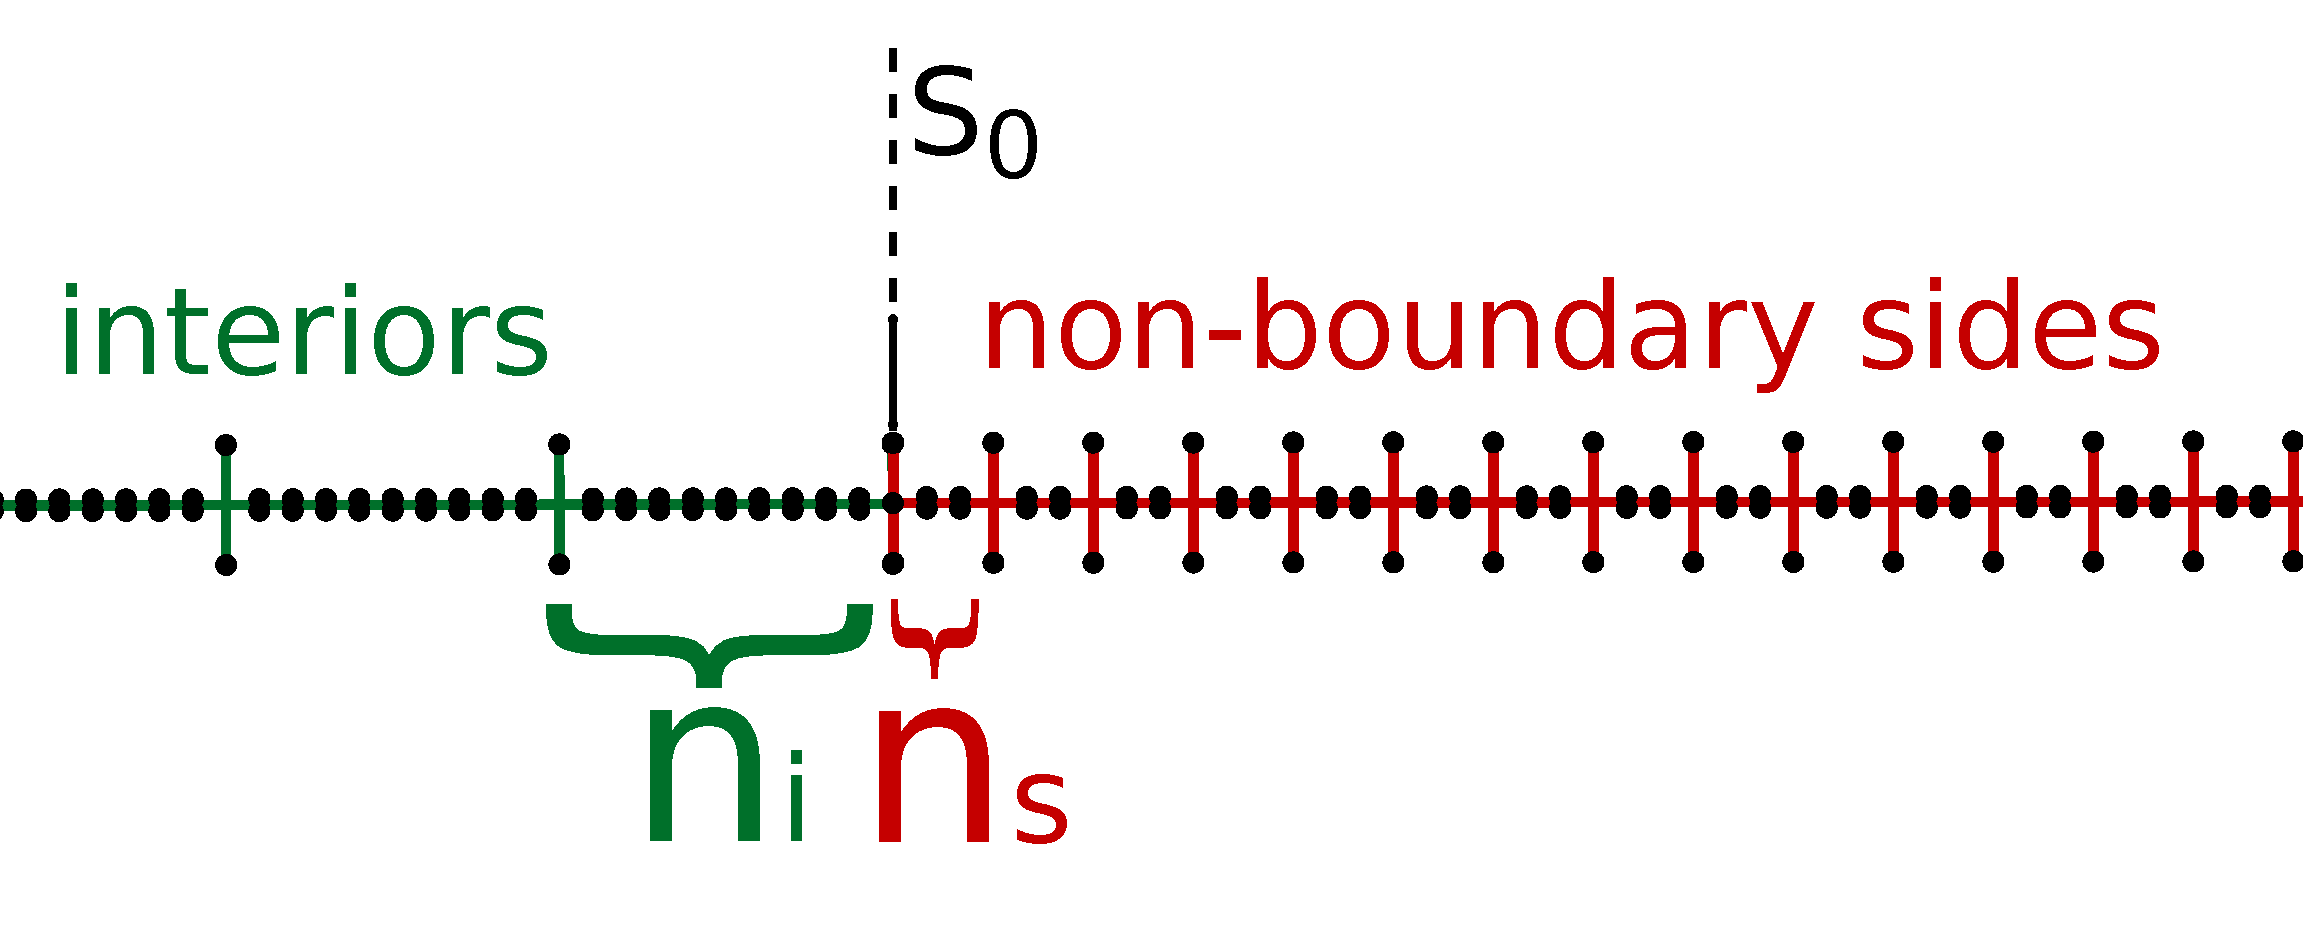
\includegraphics[width=6cm, height=2.44cm]{img/basis_layout_overall_ni_ns_s0.pdf}}
    \column{.5\textwidth}
      \small
      Let \textcolor{blue}{\large $n_i$} and \textcolor{blue}{\large $n_s$} be the count of monomials per interior and side.
      {\scriptsize We assume that the counts do not vary between sides, which is always true for any WG method using
      $P_k$ style polynomials, or for $Q_k$ polynomials over rectangle meshes.}
  \end{columns}
  \begin{itemize}[<+->]
    \item {\texttt{\textcolor{blue}{is\_int\_supported(i)\\ is\_side\_supported(i)}}}\\
      The first side-supported basis element is at index\\
      $\quad s_0 = $ {\texttt{\textcolor{blue}{ mesh.\textbf{\textcolor{orange}{num\_fes}()}}} * $n_i\quad$}\textcolor{gray}{(using 0-based indexing)},\\
      so if $i < s_0$ then element $i$ is interior supported, else side supported.
    \item {\texttt{\textcolor{blue}{num\_els()}}}: The total number of basis elements is\\
        $\quad s_0 \;+ $ {\texttt{\textcolor{blue}{ mesh.\textbf{\textcolor{orange}{num\_nb\_sides}()}}} * $n_s$}.
  \end{itemize}
\end{frame}


\begin{frame}
  \frametitle{Implementing the Basis -- Global to Local Translation}
  \frame{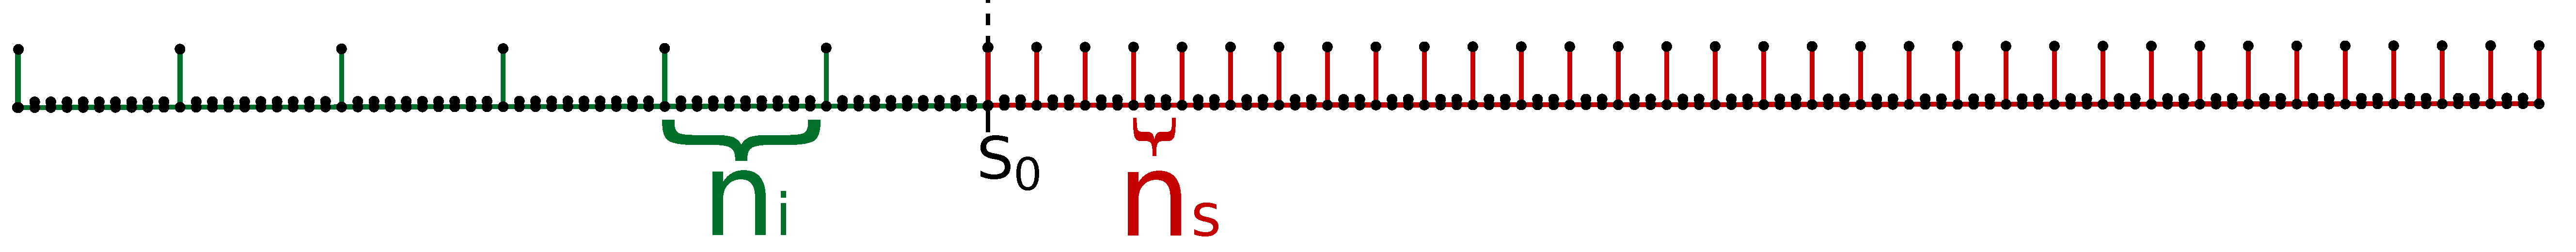
\includegraphics[width=7.3cm, height=.73cm]{img/basis_layout_overall_ni_ns_s0_thin.pdf}}
  \pause
  After using {\small \texttt{\textcolor{blue}{is\_int\_supported(i), is\_side\_supported(i)}}}, we can then use the following
    functions to translate from the global basis element number to the supporting interior or non-boundary side number,
    and shape function monomial: 
  \pause
  \begin{align*}
    \text{\texttt{\textcolor{blue}{support\_int\_fe\_num(i)}}} &= i \bdiv n_i \\
    \text{{\texttt{\textcolor{blue}{int\_rel\_mon\_num(i)}}}}   &= i \bmod n_i \\
    \text{\texttt{\textcolor{blue}{support\_nb\_side\_num(i)}}} &= (i - s_0) \bdiv n_s \\
    \text{\texttt{\textcolor{blue}{side\_rel\_mon\_num(i)}}} &= (i - s_0) \bmod n_s
  \end{align*}
  \pause
  \uncover<+-> {
    \small  
      The non-boundary side number $\textcolor{blue}{n} = \text{\scriptsize \textcolor{blue}{support\_nb\_side\_num(i)}}$ can be translated
      to two finite element/side face pairs via
      {\scriptsize \texttt{\textcolor{blue}{mesh.\textcolor{orange}{fe\_inclusions\_of\_nb\_side}(n)}}}.
    \uncover<+-> {
      Next we take either of these fe/sf pairs, obtain the oriented shape {\scriptsize \textcolor{blue}{oshape} =}
      {\scriptsize \texttt{\textcolor{blue}{mesh.\textbf{\textcolor{orange}{oriented\_shape\_for\_fe}(fe)}}}}, and then the side's
      dependent dimension via 
      {\scriptsize \texttt{\textcolor{blue}{mesh.\textbf{\textcolor{orange}{dependent\_dim\_for\_oshape\_side}(oshape, sf)}}}},
      which determines the sequence of monomials to index into for the actual monomial (one of our pre-calc seqs).
    }
  }
\end{frame}


\begin{frame}
  \frametitle{Implementing the Basis -- Local to Global Translation}
  \frame{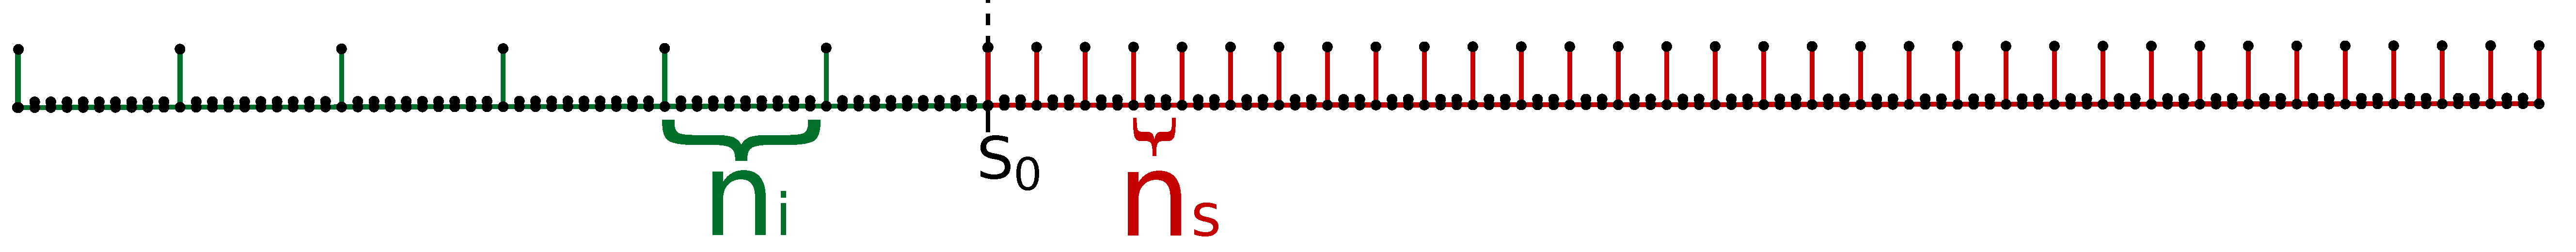
\includegraphics[width=12cm, height=1.2cm]{img/basis_layout_overall_ni_ns_s0_thin.pdf}}
  \pause
  Now we perform the ``inverse'' operations to the $\bdiv$/$\bmod$ calculations above, so we can convert from local representations back to
  to the global basis element numbers.
  \pause
  \begin{align*}
    \text{\texttt{\textcolor{blue}{int\_mon\_el\_num({fe, monn})}}} &= fe \cdot n_i + monn \\
    \text{\textcolor{blue}{nb\_side\_mon\_el\_num({n, monn})}} &= s_0 + n \cdot n_s + monn\\
    \text{\texttt{\textcolor{blue}{fe\_side\_mon\_el\_num({fe, side\_face, monn})}}} &= s_0 + n \cdot n_s + monn\\
      \text{where } \text{\textcolor{blue}{n}} = 
      \text{\textcolor{blue}{mesh.\textcolor{orange}{nb\_side\_num\_for\_fe\_side}(fe, side\_}}&\text{\textcolor{blue}{face) }}
        \text{in the latter}.
  \end{align*}
\end{frame}

\subsection{Computing Weak Gradients}

\subsubsection{WGRAD Definitions}

\begin{frame}
  \frametitle{Computing Weak Gradients -- WGRAD Definitons}
  If $v$ is a function on a finite element $T$, then its weak gradient of degree $r$ on $T$
  is defined to be the $\nabla_w v$ in $[P_r(T_0)]^d$ satisfying:\\
  \vspace{-0.25cm}
  \begin{equation*}
    (\nabla_w v, q)_{T_0} = -(v, \nabla \cdot q)_{T_0} + \langle v, q \cdot n \rangle_{\partial T}, \;\; \forall q \in [P_r(T)]^d
    \;\text{\scriptsize (\textbf{WGRAD-DEF})}
  \end{equation*}
  \pause
  
  If $B=\{b_i\}_i$ is a basis for $[P_r(T)]^d$, then we can use instead the equivalent definition:
  \begin{equation*}
    (\nabla_w v, b)_{T_0} = -(v, \nabla \cdot b)_{T_0} + \langle v, b \cdot n \rangle_{\partial T}, \;\; \forall b \in B 
    \;\quad\quad \text{\scriptsize (\textbf{WGRAD-DEF-B})}
  \end{equation*}
  \pause
  \begin{block}{Proof of Equivalence}
    \small
    That {\scriptsize \textbf{WGRAD-DEF}} implies {\scriptsize \textbf{WGRAD-DEF-B}} is obvious. Now let $q \in [P_r(T)]^d$ be
    arbitrary, and assume that {\scriptsize \textbf{WGRAD-DEF-B}} holds. Then $q = \sum_i {a_i b_i}$ for some $a_i$. If we take
    the same ${a_i}$-linear combination of the {\scriptsize \textbf{WGRAD-DEF-B}} equations with the $b_i$ in place of $b$,
    and then use the linearity of the right side of each inner product involving the $b_i$'s, we obtain the 
    {\scriptsize \textbf{WGRAD-DEF}} equation.
  \end{block}
\end{frame}

\subsubsection{The Linear System}

\begin{frame}
  \frametitle{Computing Weak Gradients -- The Linear System}
  \begin{equation*}
    (\nabla_w v, b)_{T_0} = -(v, \nabla \cdot b)_{T_0} + \langle v, b \cdot n \rangle_{\partial T}, \;\; \forall b \in B 
    \;\quad\quad \text{\scriptsize (\textbf{WGRAD-DEF-B})}
  \end{equation*}
  \pause
  \begin{itemize}[<+->]
    \item Since $\{b_i\}_i$ are a basis for $[P_r(T)]^d$ and $\nabla_w v \in [P_r(T_0)]^d$, we must have
      $\nabla_w v = \sum_j {\eta_j b_j}$ on $T_0$ for some uknowns $\eta_j$.
      Putting the latter expression for $\nabla_w v$ and also each $b_i$ in place of $b$ in turn into
      {\scriptsize \textbf{WGRAD-DEF-B}}, we obtain a system of linear equations, which we can solve for
      the unknown coefficients $\eta_j$ of our vector monomials. 
    \item The system matrix at $(i,j)$ is given by\\ $M_{i,j} = (b_j, b_i)_{T_0}$
    \item The $i^{\text{th}}$ component of the right hand side vector is 
      $r_i = -(v, \nabla \cdot b_i)_{T_0} + \langle v, b_i \cdot n \rangle_{\partial T}$
  \end{itemize}
\end{frame}

\subsubsection{System Basis}

\begin{frame}
  \frametitle{Computing Weak Gradients -- System Basis}
  We now need to choose a specific basis $B=\{b_i\}$ for $[P_r(T)]^d$ so we can form our linear system as described above.\\
  \pause
  Let $m_1,\dots,m_m$ be the interior-relative monomials of degree $\le r$ on $T$. Then we choose our basis,
  among many possibilities, to be the following sequence of \emph{\textbf{vector monomials}} on $T$:
  \begin{align*}
    &(m_1,0,0,0,\dots,0), (m_2,0,0,0,\dots,0), \dots, (m_m,0,0,0,\dots,0),\\
    &(0,m_1,0,0,\dots,0), (0,m_2,0,0,\dots,0), \dots, (0,m_m,0,0,\dots,0),\\
    &(0,0,m_1,0,\dots,0), (0,0,m_2,0,\dots,0), \dots, (0,0,m_m,0,\dots,0),\\
    &\dots\\
    &(0,\dots,0,m_1), (0,\dots,0,m_2), \dots, (0,\dots,0,m_m)
  \end{align*}
  \pause
  Each of these vector monomials has a $T$-interior-relative monomial in one component, and the constantly $0$ function in
  every other component.  The vector monomials are ordered so that reassembling a solution into a composite vector polynomial
  will be easy. 
\end{frame}

\subsubsection{Inputs}
 
\begin{frame}
  \frametitle{Computing Weak Gradients -- Inputs}
  \begin{equation*}
    (\nabla_w v, b)_{T_0} = -(v, \nabla \cdot b)_{T_0} + \langle v, b \cdot n \rangle_{\partial T}, \;\; \forall b \in B 
    \;\quad\quad \text{\scriptsize (\textbf{WGRAD-DEF-B})}
  \end{equation*}
  \pause
  \begin{itemize}[<+->]
    \item  We compute weak gradients \emph{\textbf{only for main basis shape functions}}.
    \item We lose no generality by doing this, because:
      \begin{enumerate}[<+->]
        \item Any WG approximation function is a linear combination of the main basis shape functions.
        \item It's clear from {\scriptsize \textbf{WGRAD-DEF-B}} that the solution for a linear combination $v = \sum_i a_i v_i$
          is the same linear combination of the individual solutions, $\nabla_w v = \sum_i a_i \nabla_w v_i$.
          Which is to say that the weak gradient operator is linear.
      \end{enumerate}
    \item Also since both a shape function and our vector monomial basis use coordinate systems defined relative to faces of the finite
      element, the actual position of the finite element does not matter in the calculation.
      So \emph{\textbf{all computations can be done on an oriented shape}} instead of the individual elements having the shape.
  \end{itemize}
\end{frame}


\begin{frame}
  \frametitle{Computing Weak Gradients -- Input Batching}
  If a set of shape functions are supported on the faces of the same oriented shape, then all of their weak gradients
  can be computed by solving a \emph{\textbf{single linear system}}. This is because:
  \pause
  \begin{itemize}[<+->]
    \item The system matrix $M_{i,j} = (b_j, b_i)_{T_0}$ used to compute each weak gradient is the same, only depending
      on the shape of interior $T_0$ and the fixed basis of vector monomials.
    \item Solving multiple systems $M\,x_j = r_j$ {\scriptsize $(j=1,\dots,q)$} for column vectors $x_j$ and $r_j$
      is equivalent to solving a single system $M\,X = R$ for \emph{matrices}
      $X = (x_1|x_2|\dots|x_q)$, and $R = (r_1|r_2|\dots|r_q)$.
  \end{itemize}
  \uncover<+-> {
    \frame{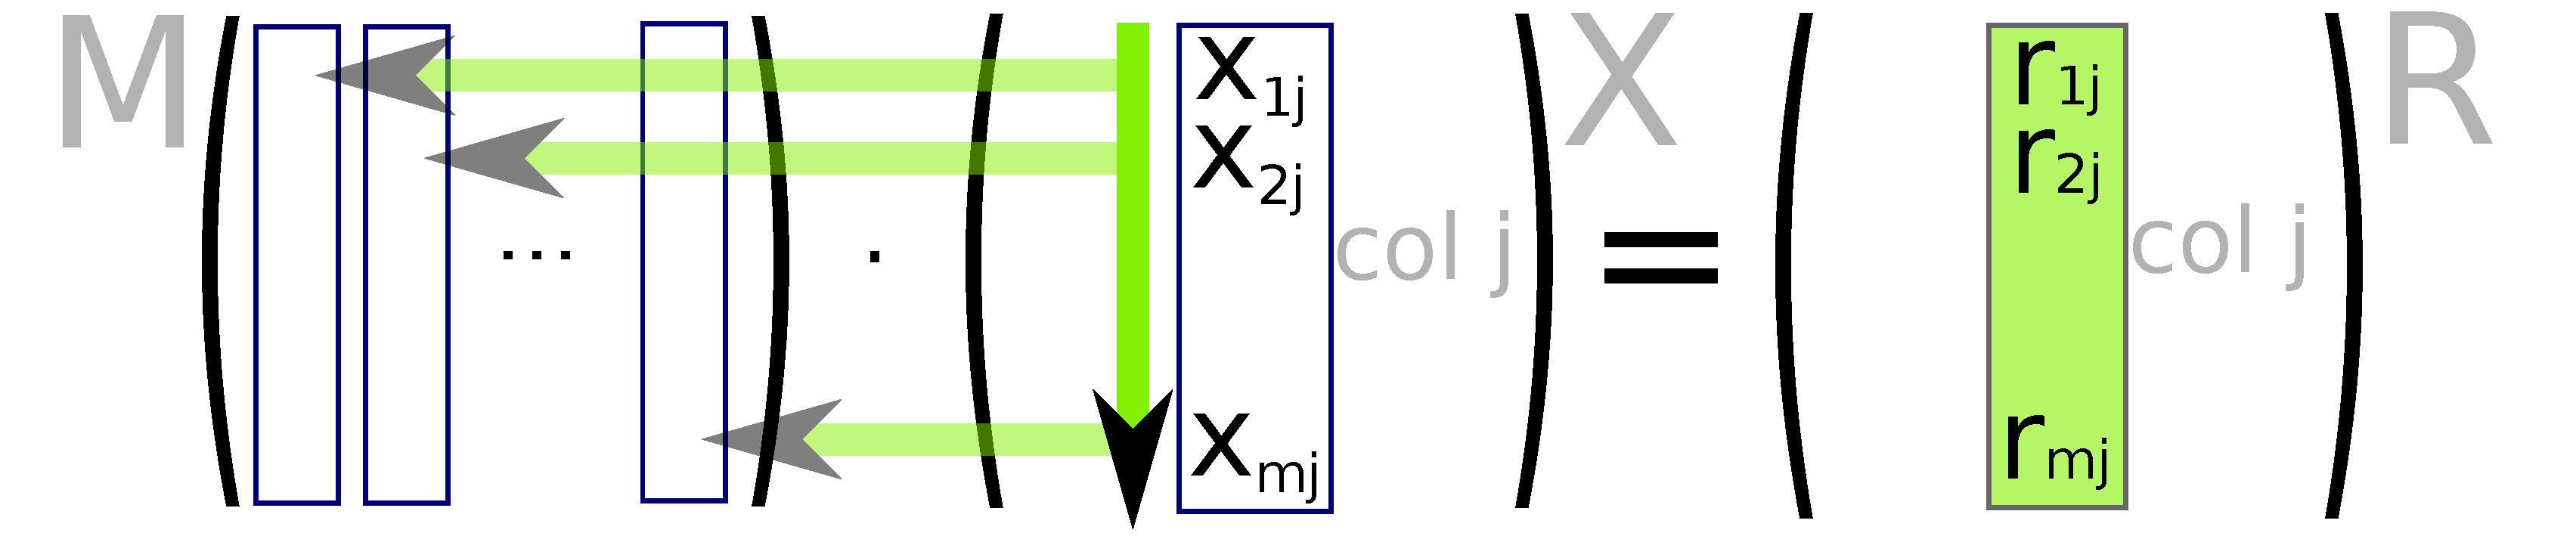
\includegraphics[width=12cm, height=2.5cm]{img/matrix_matrix_sys.pdf}}
    \uncover<+-> {
      By stacking right hand sides for the shape functions as the columns of $R$, we can solve for all the shape functions at once on 
      the shape.
    }
  }
\end{frame}

\subsubsection{Final Interface}

\begin{frame}
  \frametitle{Computing Weak Gradients -- Final Interface}
  The final interface to our our weak gradient solver consists of a constructor function and a solver function:\\ 
  \pause
  \begin{itemize}[<+->]
    \item  \textcolor{blue}{new}(\textcolor{blue}{comp\_mons\_deg\_lim}, \textcolor{blue}{mesh}) $\; \rightarrow$ {\small WeakGradSolver}\\
      For the ``optimal combination'' WG method the degree limit should be $k-1$.
      The mesh is also provided to this constructor function so the solver object can pre-compute and store the vector monomial
      inner products matrices (system matrices) for each oriented shape of the mesh.
    \item The actual weak gradient computation function:\\
      \textcolor{blue}{wgrads\_on\_oshape}(\\
      \hspace{.5cm} \textcolor{blue}{int\_mons}: [Mon],\\
      \hspace{.5cm} \textcolor{blue}{side\_mons\_by\_sideface}: [[Mon]], \textcolor{gray}{\scriptsize // mon seq for side face s at index s}\\
      \hspace{.5cm} \textcolor{blue}{oshape},\\
      \hspace{.5cm} \textcolor{blue}{mesh}\\
      ) $\rightarrow$ {\scriptsize ([WeakGrad], [[WeakGrad]])} \textcolor{gray}{\scriptsize // int mon wgrads, side mon wgrads by side face}
  \end{itemize}
\end{frame}

\subsubsection{Requirements on Other Modules}

\begin{frame}
  \frametitle{Computing Weak Gradients -- Reqs on Other Modules}
  \vspace{-.75cm}
  \begin{equation*}
    (\nabla_w v, b)_{T_0} = -(v, \nabla \cdot b)_{T_0} + \langle v, b \cdot n \rangle_{\partial T}, \;\; \forall b \in B 
    \;\quad\quad \text{\scriptsize (\textbf{WGRAD-DEF-B})}
  \end{equation*}
  \pause
  \textbf{Additional Mesh Functions}
  \begin{itemize}[<+->]
    \item Our system equation requires several inner products defined by integrals which only the mesh could possibly do, because they
      involve the geometry of the elements in a non-trivial way.
    \item For system matrix inner products $M_{i,j} = (b_j, b_i)_{T_0}$, we need\\
      {\small \texttt{\textcolor{blue}{mesh.\textbf{\textcolor{orange}{intg\_facerel\_mon\_on\_oshape\_int}(mon, oshape)}}}},\\
      mon being the dot product of vector monomials $b_j$ and $b_i$.
    \item For the first term of the RHS (interior supported shape function), we use also use the above new function with mon being
      the monomial part of $v \;\nabla \cdot q$ (missing scalar applied separately).
    \item For the second term of the RHS (side supported shape function):
      {\small \texttt{\textcolor{blue}{mesh.\textbf{\textcolor{orange}{intg\_siderel\_mon\_x\_intrel\_vmon\_dot\_normal\_on\_oshape\_side}\\
      \hspace{0.5cm}(v, q, oshape, side\_face)}}}}
    \item We've also used divergence operator on vector monomials, and multiplication of monomials, both easily implemented.
  \end{itemize}
\end{frame}

\begin{frame}
  \frametitle{Computing Weak Gradients -- More Reqs on Other Mods}
 
  \vspace{-.4cm}
  \textbf{Pre-computing Weak Gradients}
  \vspace{.2cm}

  Weak gradients can be pre-computed and stored in the basis by the triplet of oriented shape, face,
    and face-relative monomial number.

  \pause
  \uncover<+-> {
  \vspace{.2cm}
  \textbf{Method:}
    The mesh is consulted to get the number of oriented shapes, and number of sides for each oriented shape. The basis
    provides shape function monomial sequences for each of these shape faces, and asks the weak gradient module to compute the
    values, which values are then stored in the basis object.
 
  \vspace{.15cm}
  \uncover<+-> {
  The pre-computed values are then made available to other modules via functions\\
    -- {\small \texttt{\textcolor{blue}{basis.\textbf{\textcolor{orange}{int\_mon\_wgrad}(monn, oshape)}}}}\\
    -- {\small \texttt{\textcolor{blue}{basis.\textbf{\textcolor{orange}{side\_mon\_wgrad}(monn, oshape, side\_face)}}}}
  }}
\end{frame}
 
\subsection{Computing Projections}

\subsubsection{The System}

\begin{frame}
  \frametitle{Computing Projections -- The System}
  \begin{columns}
    \column{.45\textwidth}
      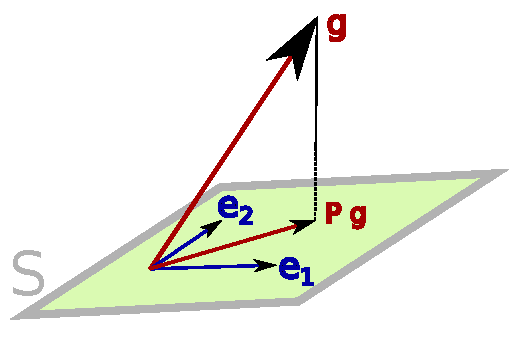
\includegraphics[width=5cm, height=3.33cm]{img/projection.pdf}
    \column{.55\textwidth}
      To project a vector $g$ onto a subspace S with basis $\{e_i\}_{i=1,\dots,m}$, we require that the projection
      $P\,g$ satisfies
      $$\langle P\,g, e_i \rangle = \langle g, e_i \rangle$$ for $i=1,\dots,m$.
  \end{columns}
  \pause

  Since $P g = \sum_j{ a_j e_j }$ for some $a_1,\dots,a_m$, this gives us a linear system, with system matrix
  $M_{i,j} = \langle e_j, e_i \rangle$, and right hand side column vector $r$ with value
  $r_i = \langle g, e_i \rangle$ at row $i$.
  \pause
 
  For our cases, $S$ will be the space of shape functions supported on a fe face, the i.p. is integration of the product
  of its input functions on the face, and the basis $\{e_i\}_i$ for $S$ is given by one of the basis functions:
  \pause
  \begin{itemize}[<+->]
    \item \texttt{\textcolor{blue}{basis.\textcolor{orange}{ref\_int\_mons}()}} 
    \item \texttt{\textcolor{blue}{basis.\textcolor{orange}{side\_mons\_for\_fe\_side}(fe, side\_face)}}
    \item \texttt{\textcolor{blue}{basis.\textcolor{orange}{side\_mons\_for\_oshape\_side}(oshape, side\_face)}}
  \end{itemize}
\end{frame}

\subsubsection{Projecting Global Functions onto Side Spaces}

\begin{frame}
  \frametitle{Projecting Global Functions onto Side Spaces}
  {\small \texttt{\textcolor{blue}{projs\_to\_span\_fes\_side\_supp\_basis\_els({\scriptsize g, fes, oshape, side\_face $\sigma$})}}}\\
  \hspace{0.5cm} $\rightarrow$ [Polynomial]\\
  \pause
  \begin{itemize}[<+->]
    \item This function performs projections of a global function \textcolor{blue}{$g$} separately onto the spaces of shape functions
      supported on the given relative side face \textcolor{blue}{$\sigma$} of the passed finite elements, which all must be of the
      same indicated oriented shape.  A projection result polynomial is returned for each of the passed finite elements.
    \item The system matrix for each of these projections is the same, given by
      $M_{i,j} = \langle e_j, e_i \rangle_{\text{oshape},\sigma}$, for which we need a new mesh function,\\
      \texttt{\small \textcolor{blue}{\textcolor{orange}{intg\_facerel\_mon\_on\_oshape\_side}(mon, oshape, side\_face)}}\\
      for the integration. Here for \texttt{\textcolor{blue}{mon}} we pass the product $e_j e_i$.
    \item The right hand sides may be stacked so that all projections are found via a single linear solve.
      Column $j$ of the combined rhs represents the projection for \texttt{\textcolor{blue}{fes(j)}}, given by
      $R_{i,j} = \langle g, e_i\rangle_{fes(j),\sigma}$, for which we need another new mesh integration function,
      $\texttt{\small \textcolor{blue}{\textcolor{orange}{intg\_global\_fn\_x\_facerel\_mon\_on\_fe\_side}(g, mon, fe, side\_face)}}$.
  \end{itemize} 
\end{frame}

\subsubsection{Projecting Interior Monomials onto Side Spaces}

\begin{frame}
  \frametitle{Projecting Interior Monomials onto Side Spaces}
  {\small \texttt{\textcolor{blue}{proj\_int\_mons\_to\_span\_oshape\_side\_supp\_basis\_els\\
    \hspace{0.5cm}(int\_mons, oshape, side\_face $\sigma$)}}} $\rightarrow$ [Polynomial]\\
  \pause
  \begin{itemize}[<+->]
    \item Need this projection in the stabilization term of $\mathfrak a_s$.
    \item Implementation is much like the previous, except we are projecting multiple functions on a single
      shape side, and the functions to be projected are defined relative to the local interior origin.
    \item The system matrix is defined just as before.
    \item We can find projections for all interior monomials with a single linear system solve, with combined right hand side
      matrix given by $R_{i,j} = \langle m_j, e_i\rangle_{\text{oshape},\sigma}$, where $m_j$ is interior monomial $j$. For this we
      need another new mesh function,
      \texttt{\scriptsize \textcolor{blue}{\textcolor{orange}{intg\_intrel\_mon\_x\_siderel\_mon\_on\_oshape\_side}(imon,smon,oshape,side\_face)}}.
    \item The right hand side integrals are done completely on the oriented shape instead of individual finite elements, which is
      possible because the monomials to be projected are defined relative to the interior origin.
  \end{itemize} 
\end{frame}

\subsection{The Main WG System}

\subsubsection{Introduction}

\begin{frame}
  \frametitle{The Main WG System -- Introduction}
    We seek approximate solution $u_h$ in the piecewise polynomial approximation space $V_h(\Omega)$ over a mesh $M$ 
    of region $\Omega$, which satisfies
    \begin{align*}
      \mathfrak{a}(u_h,v) & = (f,v)_{M_0}\quad\quad \forall{v} \in V_h^0(\Omega) \\
      u_h & = Q_b\,g \text{ on } \partial\Omega
    \end{align*}
    Here 
    \begin{itemize}[<+->]
      \item $\mathfrak{a}$ is a bilinear form which satisfies our additional \emph{\textbf{locality}} and
        \emph{\textbf{element-summability}} requirements discussed previously.
      \item The polynomials of $V_h(\Omega)$ satisfy a pair of degree constraints for the interior and side polynomial pieces. 
      \item The inner product $(f,v)_{M_0}$ is integration of the product of its operands over the union of all mesh element
        interiors, $M_0$.
      \item $Q_b\,g$ is the function which is equal on each outside boundary element side $e \subset \partial\Omega$ to the 
        $L_2$ projection of $g$ onto the subspace of $V_h(\Omega)$ supported on $e$, and which is $0$ everywhere else.
    \end{itemize}
\end{frame}
    
\subsubsection{Deriving the System}

\begin{frame}
  \frametitle{The Main WG System -- Deriving the System}
  Let $\{e_i\}_{i=1,\dots,m}$ be a basis for the 0-boundary subspace of our approximation space, $V_h^0(\Omega)$.
  Then our original system is equivalent to
  \begin{align*}
    \mathfrak{a}(u_h,v) & = (f,e_i)_{M_0}\quad\quad i=1,\dots,m \\
    u_h & = Q_b\,g \text{ on } \partial\Omega
  \end{align*}
  \pause
  Since $Q_b g$ is $0$ outside of $\partial \Omega$, and $\{e_j\}_{j=1,\dots,m}$ is a basis for $V_h^0(\Omega)$, we must have
  $$u_h = \sum_j{\eta_j e_j} + Q_b g$$
  for some unknowns $\eta_1,\dots,\eta_m.$  
  \pause
  Thus our system becomes
  $$\mathfrak{a}(\sum_j{\eta_j e_j} + Q_b g, e_i) = (f, e_i)_{M_0} \quad i=1,\dots,m$$
  which we can rearrange to \dots
\end{frame}

\subsubsection{System Final Form}

\begin{frame}
  \frametitle{The Main WG System -- System Final Form}
  \begin{block}{WG Main Linear System}
    \begin{align*}
      \sum_{j=1}^m{\mathfrak{a}(e_j, e_i) \,\eta_j} &= (f, e_i)_{M_0} - \mathfrak{a}(Q_b g, e_i), \quad i=1,\dots,m\\
      u_h &= \sum_{j=1}^m{\eta_j e_j} + Q_b g
    \end{align*}

  \end{block}  
  \pause
  This is a linear system with matrix $M$ given by $M_{i,j} = \mathfrak{a}(e_j, e_i)$, which we can solve for the unknowns
  $\eta_j$ defining $u_h$.  Note $M$ is the \emph{\textbf{transpose}} of the basis-vs-basis $\mathfrak{a}$-values matrix.\\
  \pause
  It remains to discuss:
  \begin{itemize}[<+->]
    \item the interface (set of functions) through which $\mathfrak{a}$ values are calculated,
      the vbf being another ``contract'' plugin point
    \item details of how the right hand side is calculated
    \item details of how the system matrix is built
  \end{itemize}

\end{frame}


\subsubsection{The VBF Interface}

\begin{frame}
  \frametitle{The VBF Interface}
  \vspace{-.40cm}
  \begin{align*}
    \mathfrak{a}(v,w) &= \sum_T { \spot<2->{\phi}(v|_T,w|_T) }\\
    \text{\scriptsize (\textbf{WG-SYS})} \quad \sum_{j=1}^m{\mathfrak{a}(e_j, e_i) \,\eta_j} &= (f, e_i)_{M_0} - \mathfrak{a}(Q_b g, e_i),
      \quad i=1,\dots,m
  \end{align*}
  \pause
  \begin{itemize}[<+->]
    \item From {\scriptsize WG-SYS}, we can see that we only need to implement \spot<2->{$\phi$}, and only for basis shape function inputs.
      We can use linearity to evaluate polynomial inputs.
    \item Translatability will allow us to compute on oriented shapes.
    \item Final VBF ($\phi$) interface will be\\
    \uncover<+-> {
    \texttt{\small \textcolor{blue}{int\_mon\_vs\_int\_mon(oshape, imonn1, imonn2)}}\\
    \uncover<+-> {
    \texttt{\small \textcolor{blue}{int\_mon\_vs\_side\_mon(oshape, imonn, smonn, side\_face)}}\\
    \uncover<+-> {
    \texttt{\small \textcolor{blue}{side\_mon\_vs\_int\_mon(oshape, smonn, side\_face, imonn)}}\\
    \uncover<+-> {
    \texttt{\small \textcolor{blue}{side\_mon\_vs\_side\_mon\_fe\_contr({\scriptsize oshape, smonn1, sf1, smonn2, sf2})}}\\
    \uncover<+-> {
    \texttt{\small \textcolor{blue}{is\_symmetric() }}
    }}}}}
  \end{itemize}
\end{frame}


\subsubsection{Evaluating the System RHS}

\begin{frame}
  \frametitle{Evaluating the System RHS}
  \vspace{-1.15cm}
  \begin{align*}
    \sum_{j=1}^m{\mathfrak{a}(e_j, e_i) \,\eta_j} &= \spot<2->{(f, e_i)_{M_0}} - \mathfrak{a}(Q_b g, e_i), \quad i=1,\dots,m
  \end{align*}
  
  \pause
  \uncover<+-> {
  \textbf{RHS First Term}
  \vspace{.3cm}

  \uncover<+-> {
  If basis element $i$ is not interior supported according to 
  {\small \texttt{\textcolor{blue}{basis.\textcolor{orange}{is\_int\_supported}(i)}}}, then the inner product is 0.\\
  
  \uncover<+-> {
  \vspace{.3cm}
  Else we can fetch the interior (fe) number and monomial for the basis element via
  {\small \texttt{\textcolor{blue}{basis.\textcolor{orange}{support\_int\_fe\_num}(i)}}}
  and {\small \texttt{\textcolor{blue}{basis.\textcolor{orange}{int\_mon}(i)}}}.
  
  \uncover<+-> {
  \vspace{.3cm}
  Then we perform the integration via new mesh function\\
  {\small \texttt{\textcolor{blue}{mesh.\textcolor{orange}{intg\_global\_fn\_x\_facerel\_mon\_on\_fe\_int}(f, mon, fe)}}}.
  }}}}
\end{frame}

\begin{frame}
  \frametitle{Evaluating the System RHS Contd}
  \vspace{-.29cm}
  \begin{align*}
    \sum_{j=1}^m{\mathfrak{a}(e_j, e_i) \,\eta_j} &= (f, e_i)_{M_0} - \spot<2->{\mathfrak{a}(Q_b g, e_i)}, \quad i=1,\dots,m
  \end{align*}
  
  \pause
  \uncover<+-> {
  \textbf{RHS Second Term}

  \vspace{.2cm}
  First we need to compute all projections of $g$ onto the approximation spaces over the boundary sides.
  We use a new mesh function to report boundary sides,
  {\small \texttt{\textcolor{blue}{mesh.\textcolor{orange}{boundary\_fes\_by\_oshape\_side}()}} $\rightarrow$ [[[FENum]]]}

  \uncover<+-> {
    We group the boundary sides by the side faces of the oriented shapes on which they occur, because in these groups the projections
    can be performed by solving a single linear system, via the projection module function discussed previously,\\
    {\small \texttt{\textcolor{blue}{\textcolor{orange}{projs\_to\_span\_fes\_side\_supp\_basis\_els}({\small{g,fes,oshape,side\_face}})}}}

  \uncover<+-> {
  \vspace{.1cm}
  Finally we collect the boundary projections into a \emph{map} collection by their (fe, side face) pairs, 
  allowing fast lookup by (fe, side\_face).
  }}}
\end{frame}

\begin{frame}
  \frametitle{Evaluating the System RHS Contd}
  \vspace{-.15cm}
  \textbf{RHS Second Term, Contd}
  \vspace{-.20cm}
  \begin{align*}
    \sum_{j=1}^m{\mathfrak{a}(e_j, e_i) \,\eta_j} &= (f, e_i)_{M_0} - \spot<1->{\mathfrak{a}(Q_b g, e_i)}, \quad i=1,\dots,m
  \end{align*}
  
  \uncover<+-> {
  Now we can proceed to evaluate the second term.
  There are two cases to consider, depending on whether $e_i$ is interior supported according to the mesh, via
  {\small \texttt{\textcolor{blue}{basis.\textcolor{orange}{is\_int\_supported}(i)}}}.
  
  \uncover<+-> {
  \vspace{.1cm}
  \textbf{Case 1: Basis element $e_i$ is Interior Supported}
  \vspace{.1cm}
  
  Only boundary sides which are included in the basis element's single supporting finite element can contribute to the vbf value, by the 
  \emph{\textbf{locality}} property of the variational form.

  \vspace{.1cm}
  \uncover<+-> {
  So the method for computing the vbf value will be to sum $\mathfrak{a}(p, e_i)$ over all boundary side space projections
  $p$ on the boundary sides of the supporting finite element of $e_i$, using linearity of $\mathfrak{a}$, or its per-element
  form, $\phi$.
  }}}
\end{frame}

\begin{frame}
  \frametitle{Evaluating the System RHS Contd}
  \vspace{-.15cm}
  \textbf{RHS Second Term, $e_i$ Interior Supported, Contd}
  \vspace{-.32cm}
  \begin{align*}
    \sum_{j=1}^m{\mathfrak{a}(e_j, e_i) \,\eta_j} &= (f, e_i)_{M_0} - \spot<1->{\mathfrak{a}(Q_b g, e_i)}, \quad i=1,\dots,m
  \end{align*}
  
  \uncover<+-> {
  Retrieve the local representation of the basis element $e_i$:\\
  \hspace{.2cm} {\small \texttt{\textcolor{blue}{fe \textcolor{black}= basis.\textcolor{orange}{support\_int\_fe\_num}(i)}}}\\
  \hspace{.2cm} {\small \texttt{\textcolor{blue}{oshape \textcolor{black}= mesh.\textcolor{orange}{oriented\_shape\_for\_fe}(fe)}}}\\
  \hspace{.2cm} {\small \texttt{\textcolor{blue}{$e_i$\_monn \textcolor{black}= basis.\textcolor{orange}{int\_rel\_mon\_num}(i)}}}

  \uncover<+-> {
  \vspace{.2cm}
  Then our second term is the sum of contributions to the vbf value from each side face
  $s = 1,\dots, $ \textcolor{blue}{\small mesh.\textcolor{orange}{num\_side\_faces\_for\_shape}(oshape)}.
  
  \uncover<+-> {
  The contribution from side face $s$ is $0$ if (fe,s) is not in the projections map, because then (fe,s) is not
  a boundary side.
  \uncover<+-> {
  Else if $p=\sum_j a_j m_j$ is the projection polynomial onto boundary side $s$, then $s$'s contribution is
  $\sum_j {a_j}$ * \textcolor{blue}{vbf.\textcolor{orange}{side\_mon\_vs\_int\_mon}(oshape, $m_j$, $s$, $e_i$\_monn)}.
  Here we've used linearity of the vbf over the terms of the side polynomial.
  }}}}
\end{frame}


\begin{frame}
  \frametitle{Evaluating the System RHS Contd}
  \frame{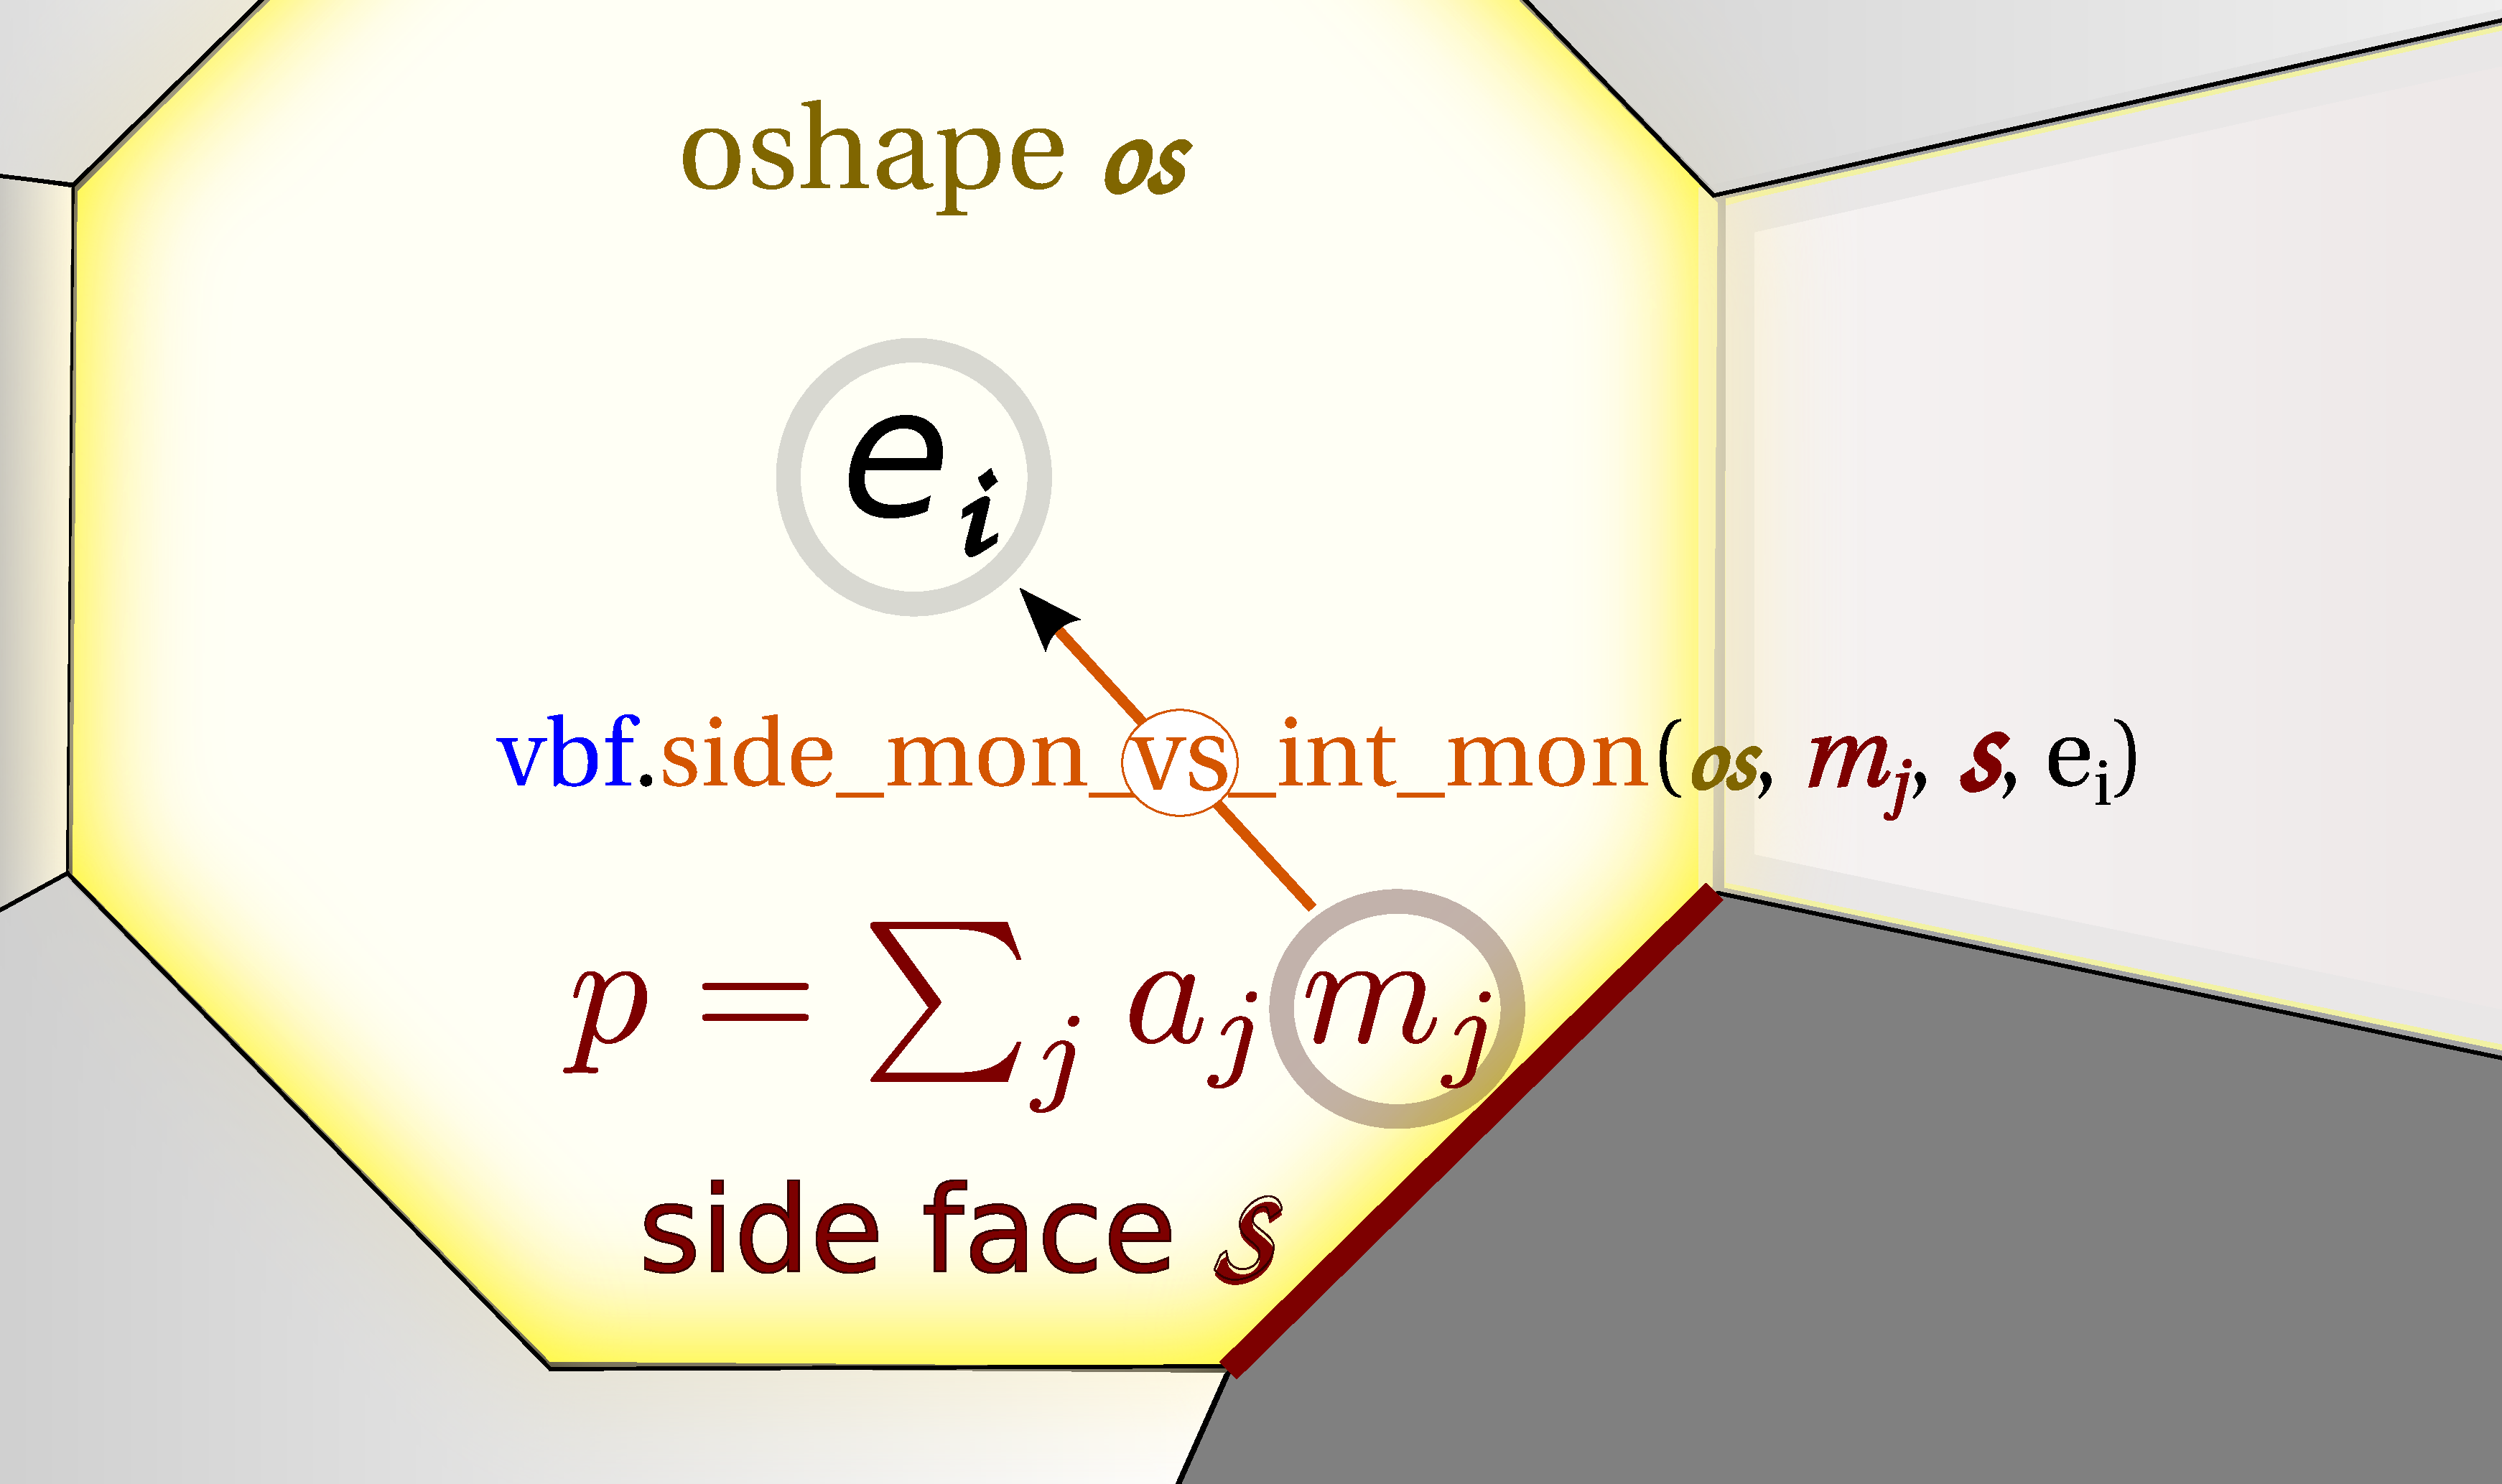
\includegraphics[width=11.5cm, height=6.84cm]{img/int_bel_bside_interaction.pdf}}
  {\scriptsize RHS second term: Boundary projection polynomial vs interior supported basis element.}
\end{frame}

\begin{frame}
  \frametitle{Evaluating the System RHS Contd}
  \vspace{-.25cm}
  \textbf{Case 2: Basis Element $e_i$ is Side Supported}
  \vspace{-.22cm}
  \begin{align*}
    \sum_{j=1}^m{\mathfrak{a}(e_j, e_i) \,\eta_j} &= (f, e_i)_{M_0} - \spot<1->{\mathfrak{a}(Q_b g, e_i)}, \quad i=1,\dots,m
  \end{align*}
  \begin{columns}
    \column{.5\textwidth}
    Only projections onto boundary side spaces from one of the two fe's which include the basis element's support side can
    possibly contribute to the vbf value, by the locality property. So let {\small (fe1, sf1), (fe2, sf2)} be the two local
    representations of $e_i$'s support side, which we obtain from the basis, via the function
    \column{.5\textwidth}
    \frame{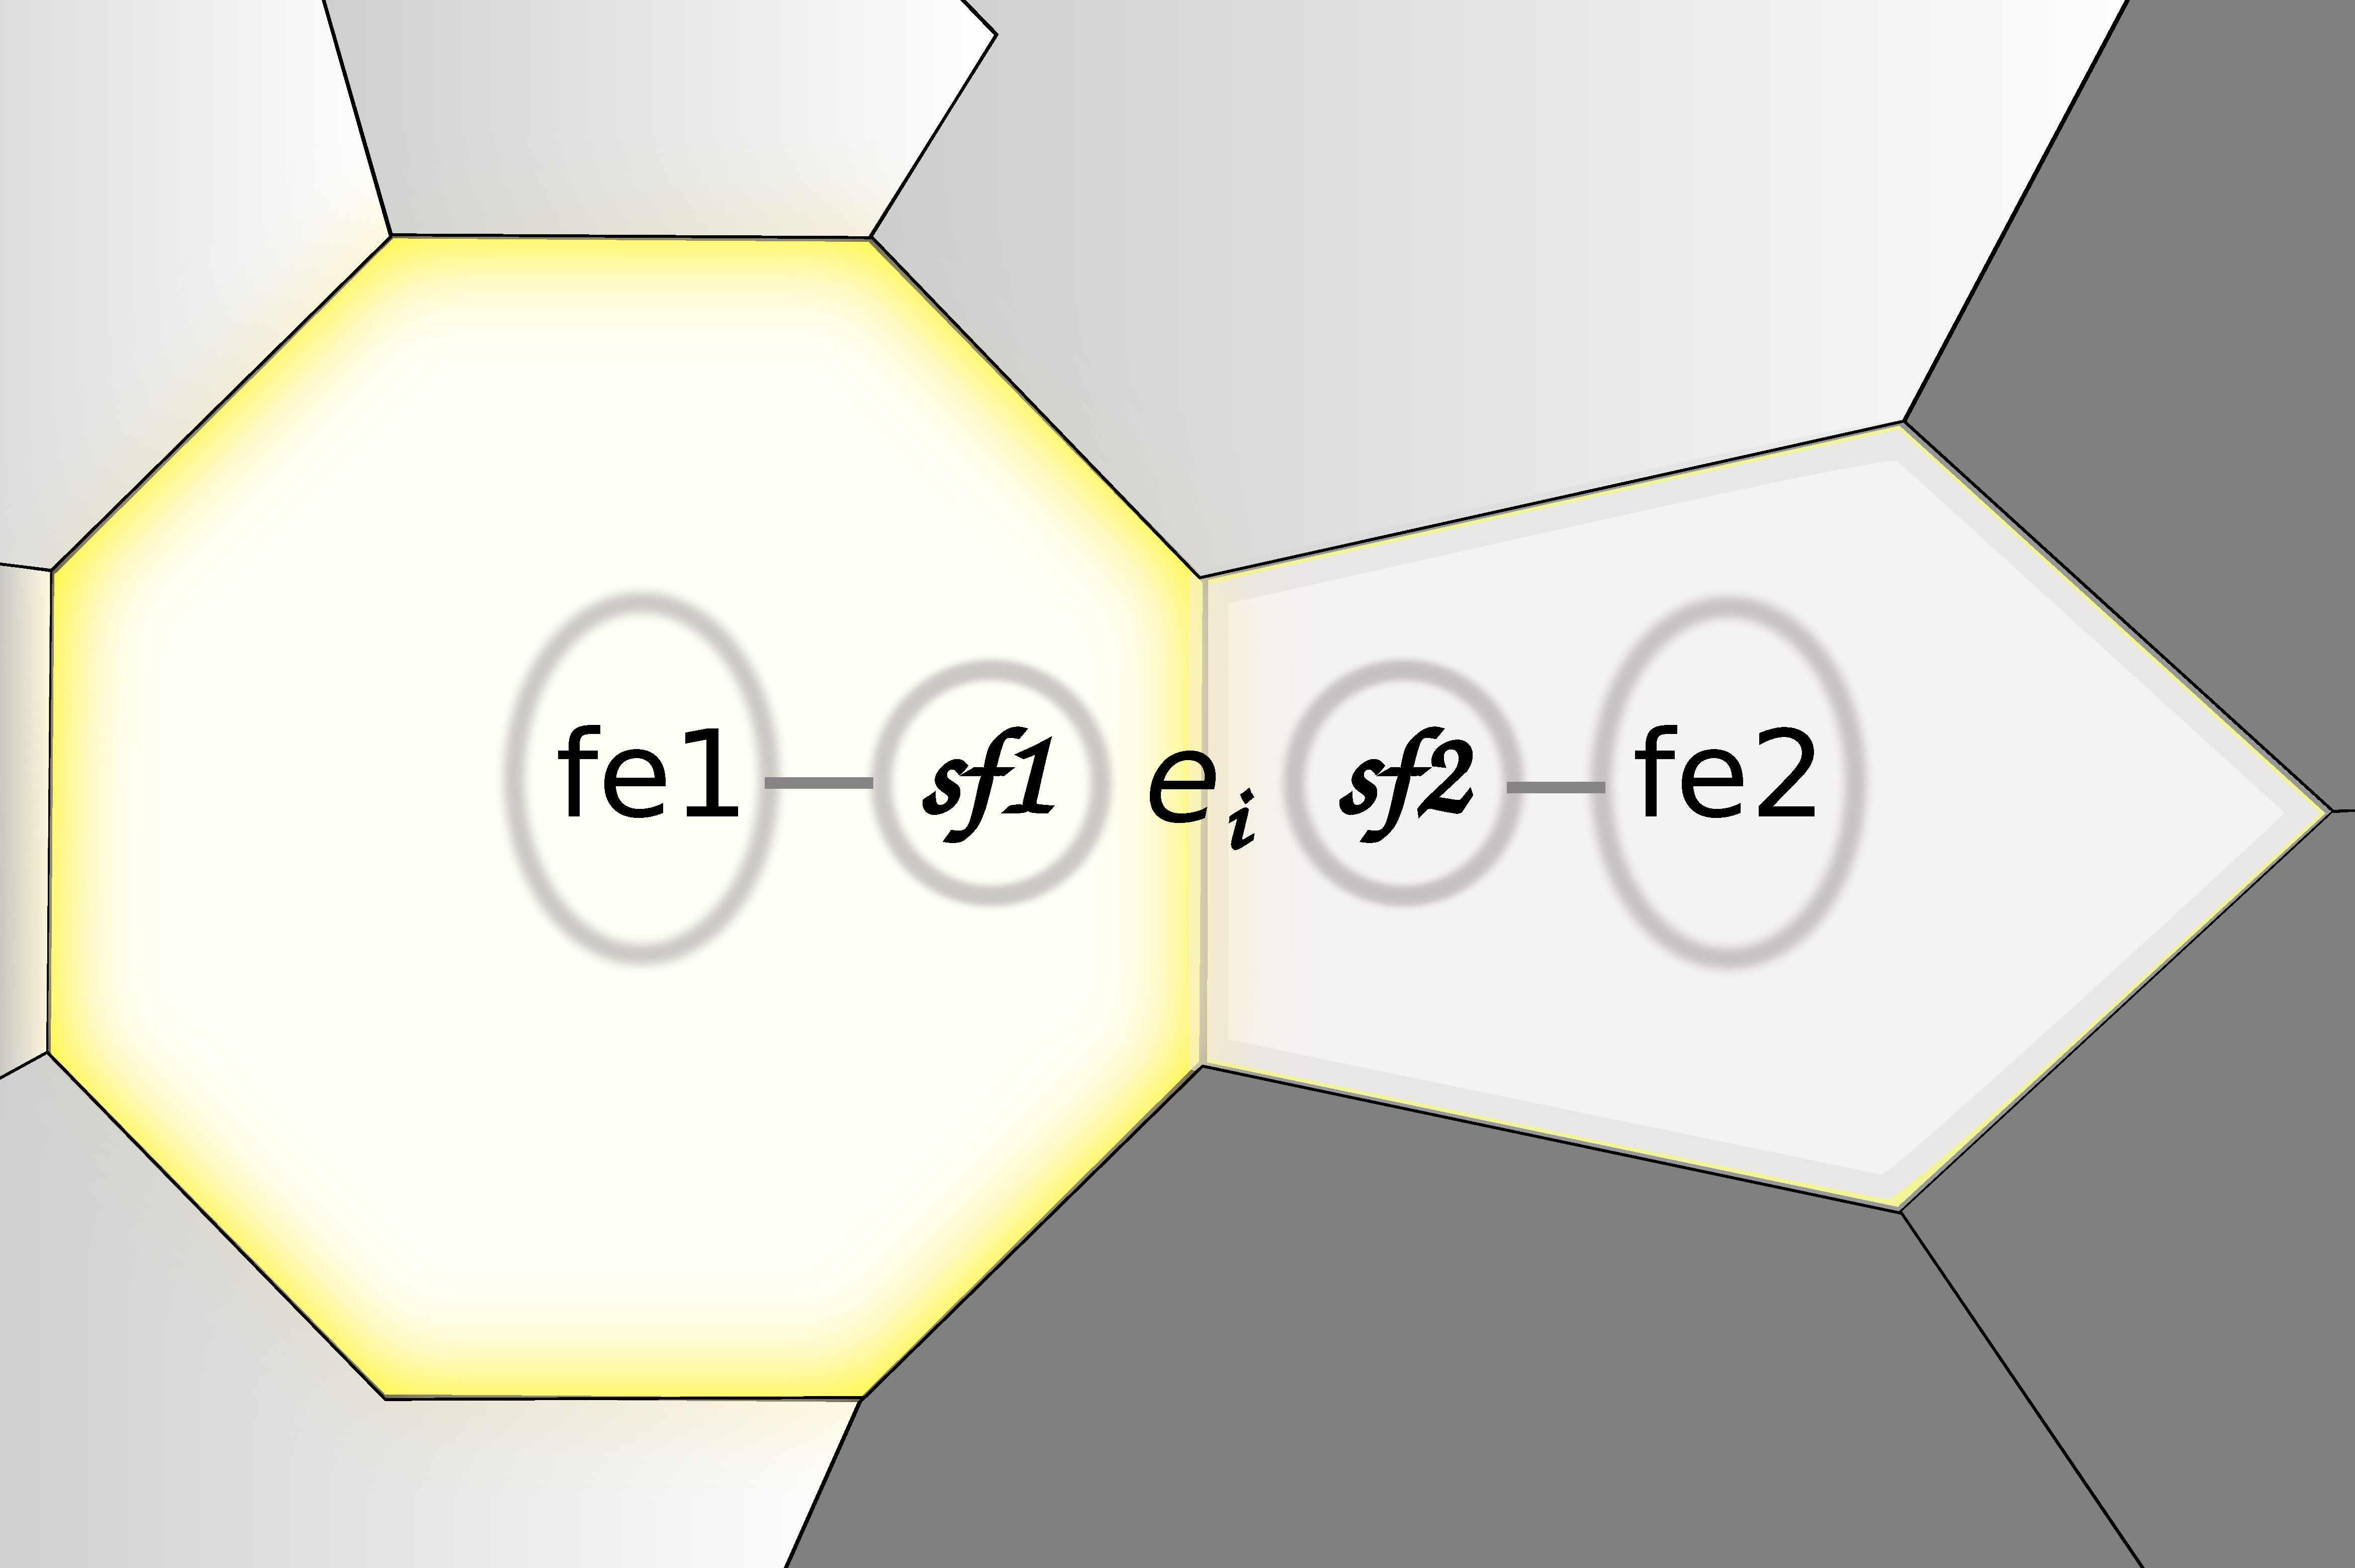
\includegraphics[width=6cm, height=4cm]{img/two_fes_side_bel_with_bsides.pdf}}
  \end{columns}
  {\small \texttt{\textcolor{blue}{basis.\textcolor{orange}{fe\_inclusions\_of\_side\_support}(i)}}}.
  \footnote{
   This is a new basis function which translates $i$ to a non-boundary side number and then defers to the mesh function
   {\scriptsize \texttt{\textcolor{blue}{mesh.\textcolor{orange}{fe\_inclusions\_of\_nb\_side}(nb\_side\_num)}}}.
  }
\end{frame}

\begin{frame}
  \frametitle{Evaluating the System RHS Contd}
  %\vspace{-.25cm}
  \textbf{Case 2: Basis Element $e_i$ Side Supported, Contd}
  \vspace{-.15cm}
  \begin{align*}
    \sum_{j=1}^m{\mathfrak{a}(e_j, e_i) \,\eta_j} &= (f, e_i)_{M_0} - \spot<1->{\mathfrak{a}(Q_b g, e_i)}, \quad i=1,\dots,m
  \end{align*}
  Then for (fe, $e_i$\_sf) in \{(fe1, sf1), (fe2, sf2)\},
  we sum the contributions from fe's boundary sides against basis element $e_i$ on side face $e_i$\_sf, and form the total
  vbf value from the sum over the two finite elements.
  
  The contribution for a boundary side projection polynomial $p=\sum_j a_j m_j$ is itself the sum of its term contributions,\\ 
  $a_j$ {\small \texttt{\textcolor{blue}{vbf.\textcolor{orange}{side\_mon\_vs\_side\_mon\_fe\_contr}(os,$m_j$,p\_sf,$e_i$\_monn,$e_i$\_sf)}}},
  where p\_sf is the side face of $p$'s support in fe, 
  \textcolor{blue}{\small $e_i$\_monn} = {\small \texttt{\textcolor{blue}{basis.\textcolor{orange}{side\_rel\_mon\_num}(i)}}} is
  $e_i$'s face-relative monomial number, and 
  \textcolor{blue}{\small os} = {\small \texttt{\textcolor{blue}{mesh.\textcolor{orange}{oriented\_shape\_for\_fe}(fe)}}} is the 
  oriented shape for fe.

  The total of all such contributions is the second term.
  \footnote{Note that this method will never double-count a boundary side's contribution, because a boundary side can only belong
   to a single finite element.}

\end{frame}


\begin{frame}
  \frametitle{Evaluating the System RHS Contd}
  \alt<-1> {\frame{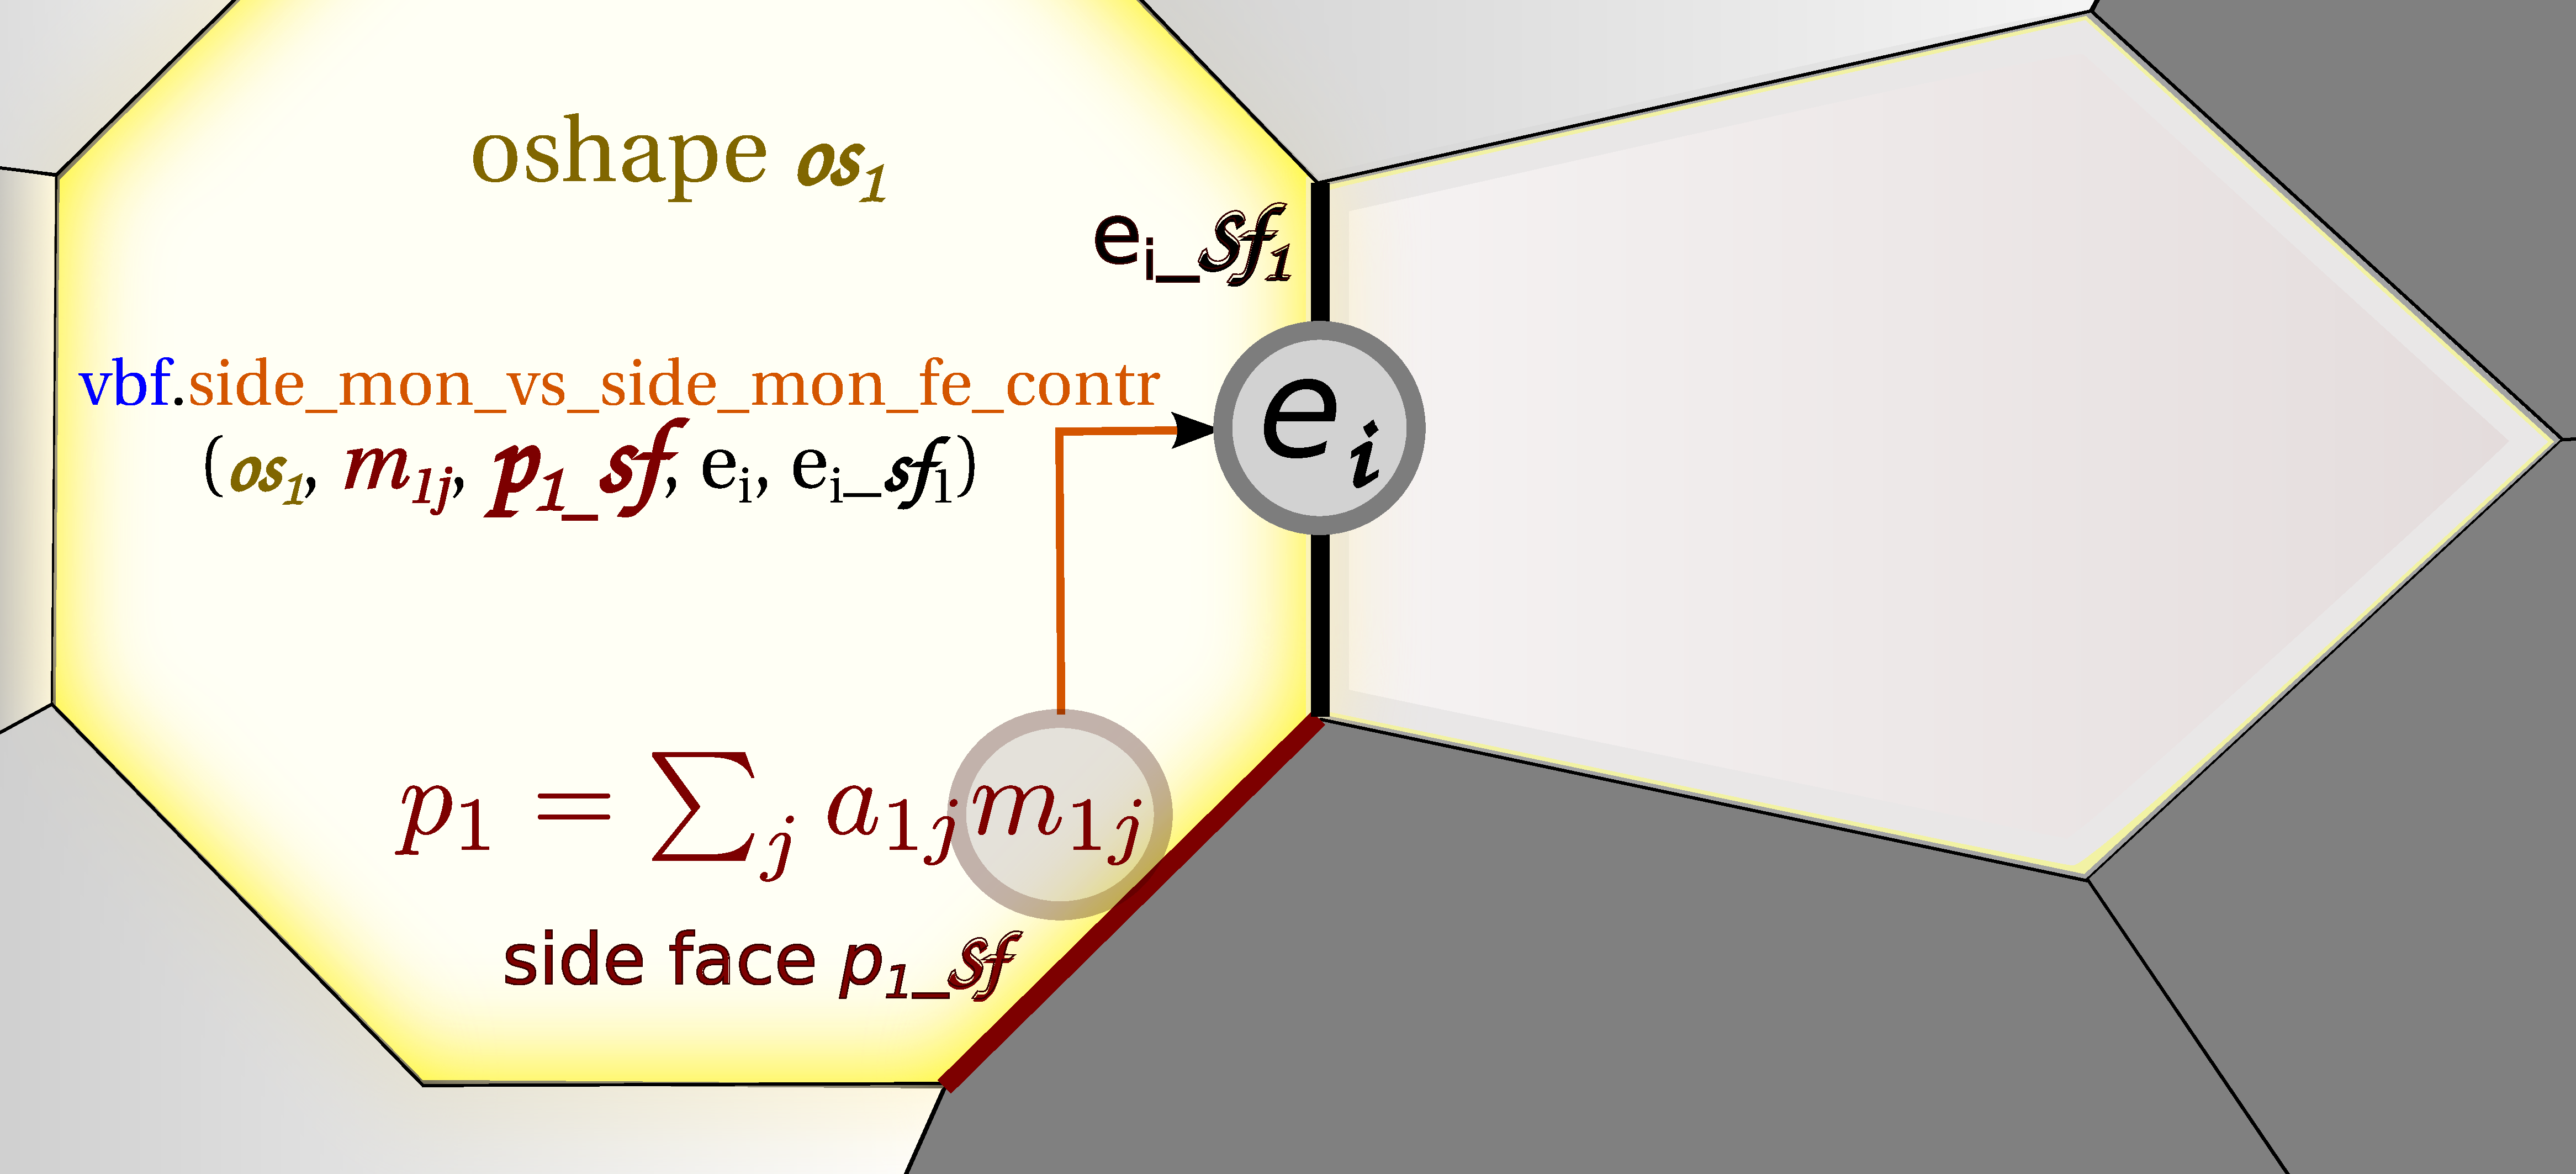
\includegraphics[width=11.5cm, height=5.24cm]{img/side_bel_bsides_interaction_left_only.pdf}}}
           {\frame{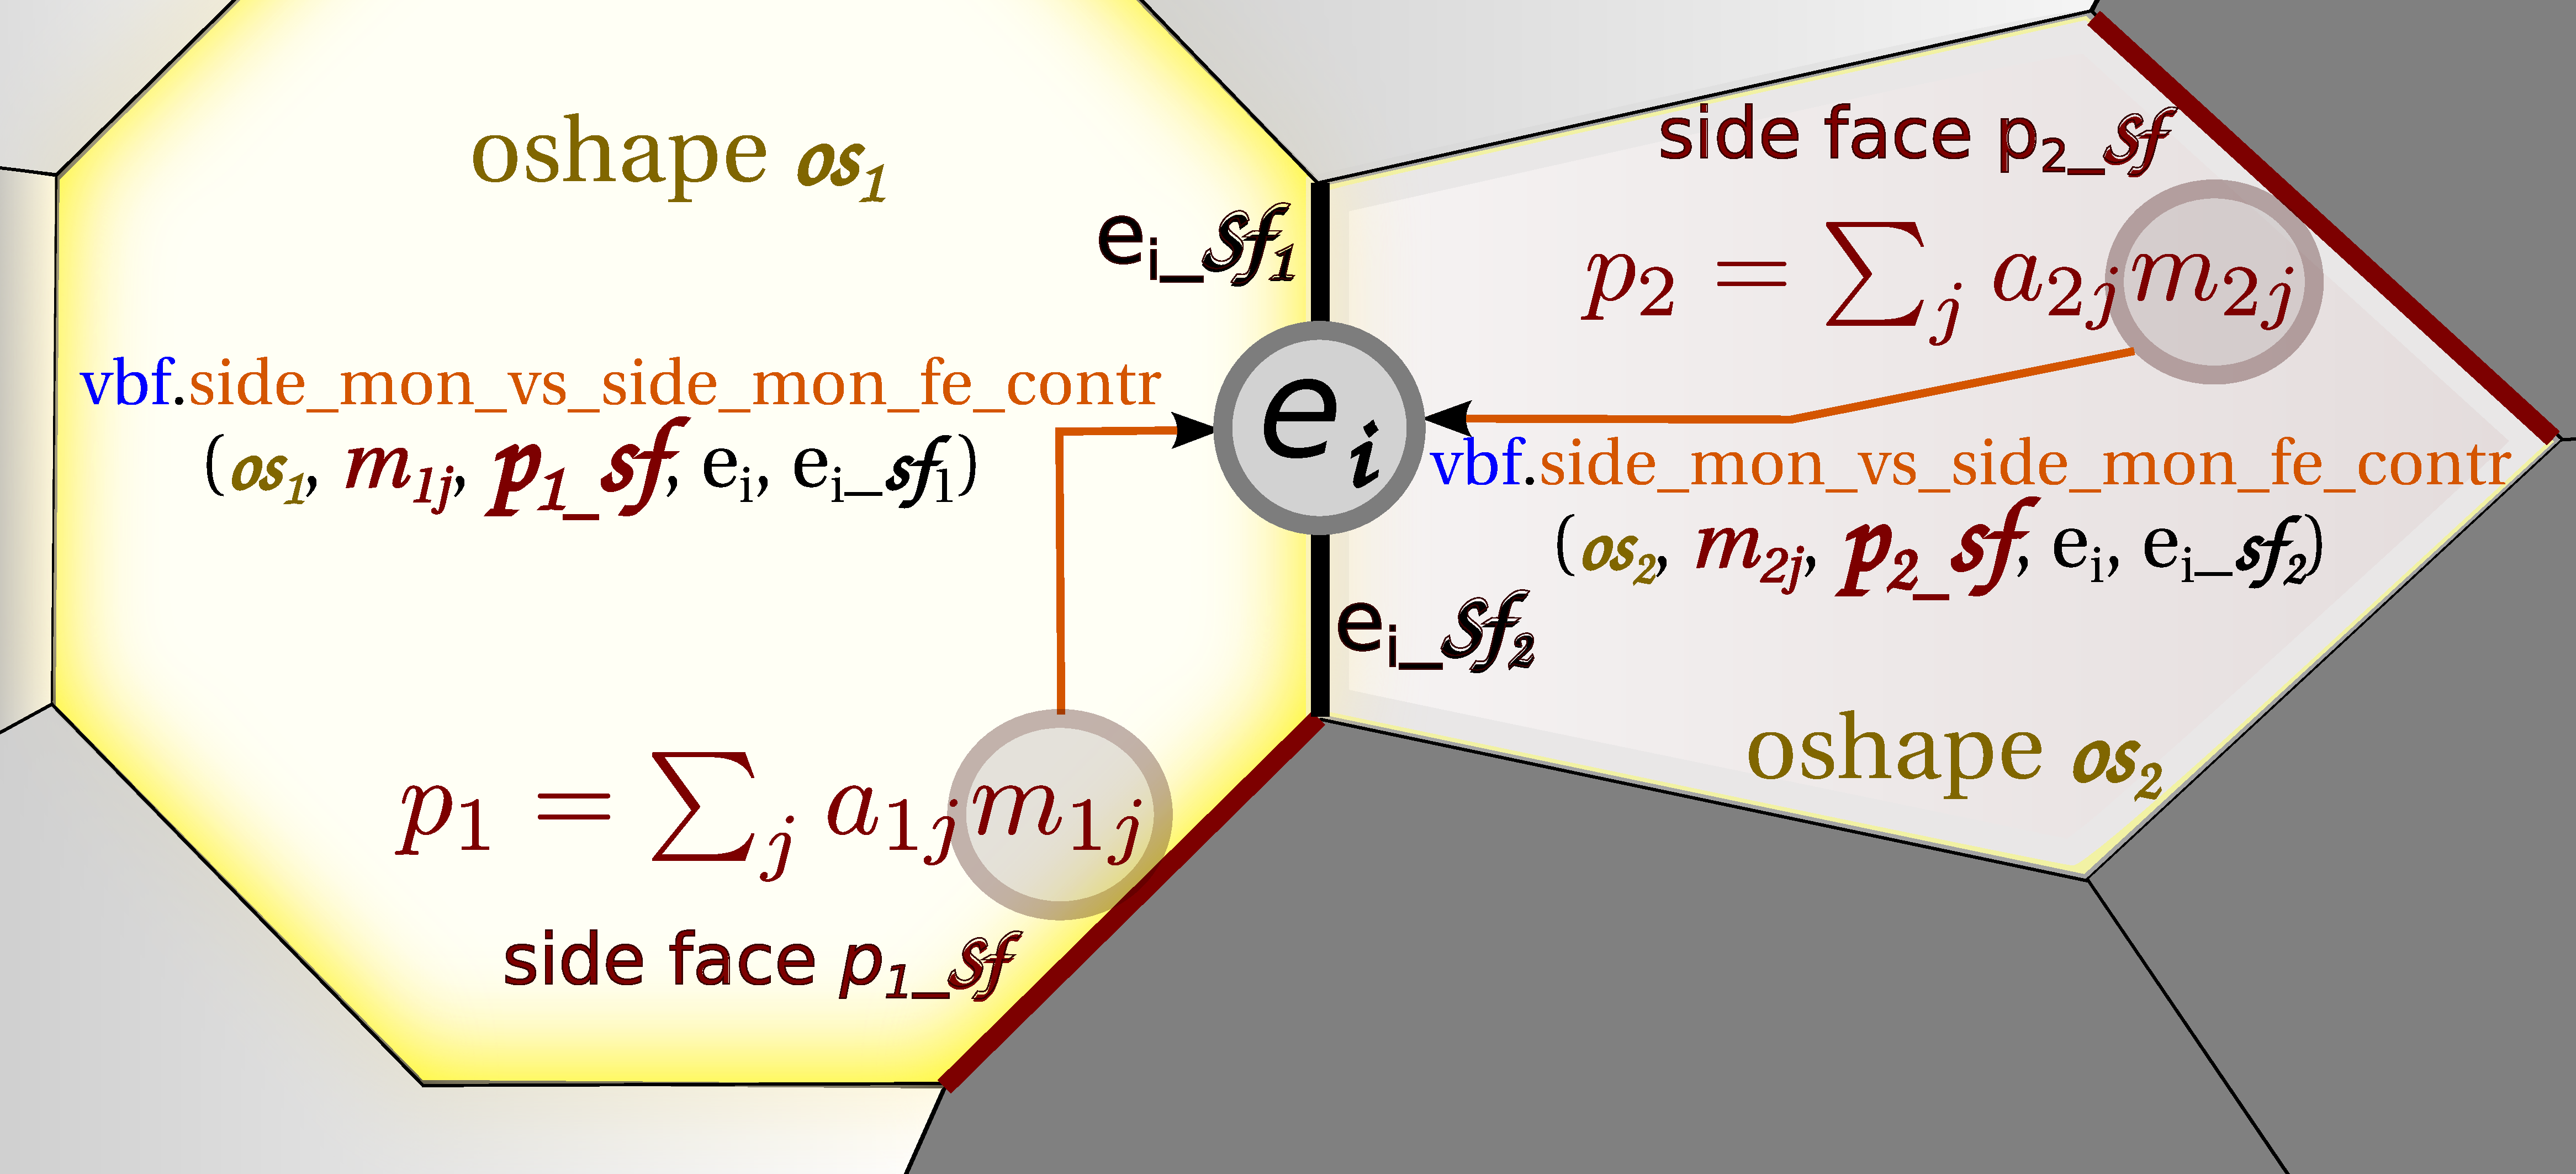
\includegraphics[width=11.5cm, height=5.24cm]{img/side_bel_bsides_interaction.pdf}}}
  {\scriptsize RHS second term: Boundary projection polynomials vs side supported basis element.}
  \pause 
\end{frame}

\subsubsection{The System Matrix}

\begin{frame}
  \frametitle{The System Matrix -- Approach}
  \textbf{Naive Approach}

  As seen previously, even among relatively small problems the number of \emph{pairings} of basis elements quickly becomes unmanageable.
  
  \pause
  \vspace{.15cm}
  \uncover<+-> {
  For $k=3$ and an 85 $\times$ 85 rectangle mesh, there are 115,090 basis elements and \emph{13,245,708,100} pairings of elements.

  \vspace{.15cm}
  \uncover<+-> {
    \begin{columns}
      \column{.95\textwidth}
        \frame{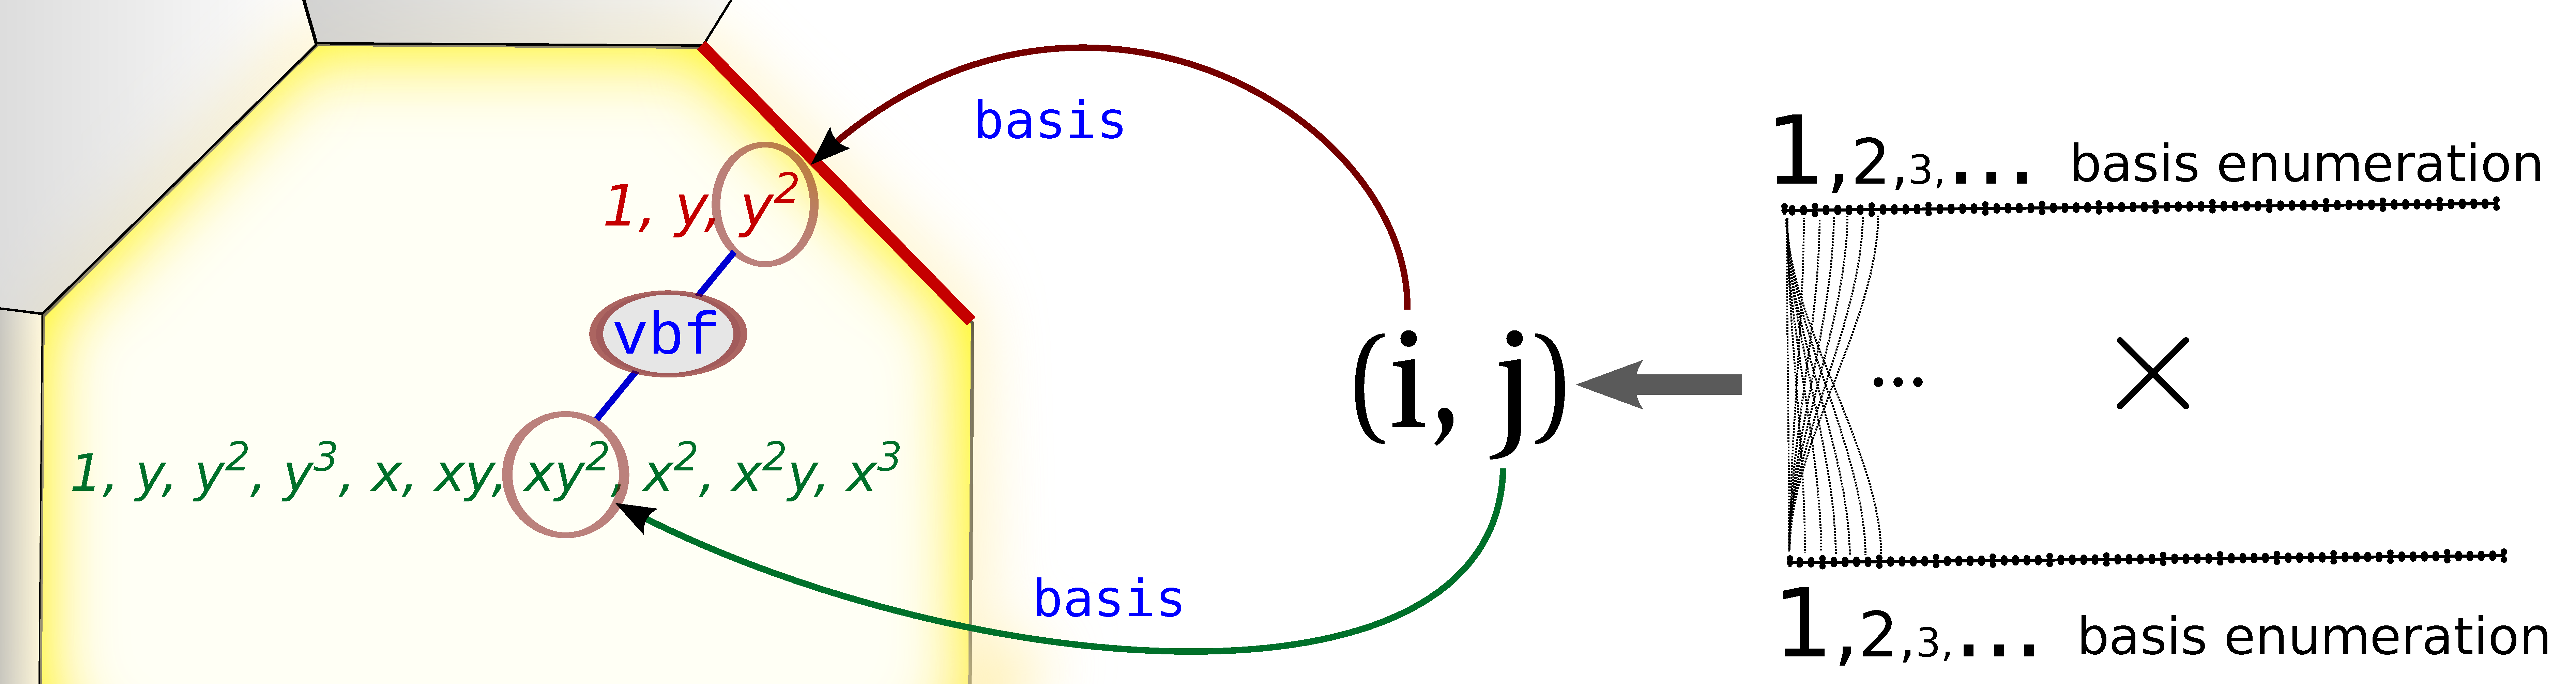
\includegraphics[width=11cm, height=2.92cm]{img/sysmatrix_basis_vs_basis_impractical.pdf}}
      \column{.05\textwidth}
        \textbf{\textcolor{red}{\Large{X}}}
    \end{columns}
  
  \vspace{.15cm}
  This rules out filling the matrix in the naive way of working backwards from each pair of basis element numbers to a pair of local
  representations, and then calculating the vbf value from the local representations if they overlap at any finite elements.
  }}
\end{frame}

\begin{frame}
  \frametitle{The System Matrix -- Approach, Contd}
  \textbf{More Scalable Approach}
  \frame{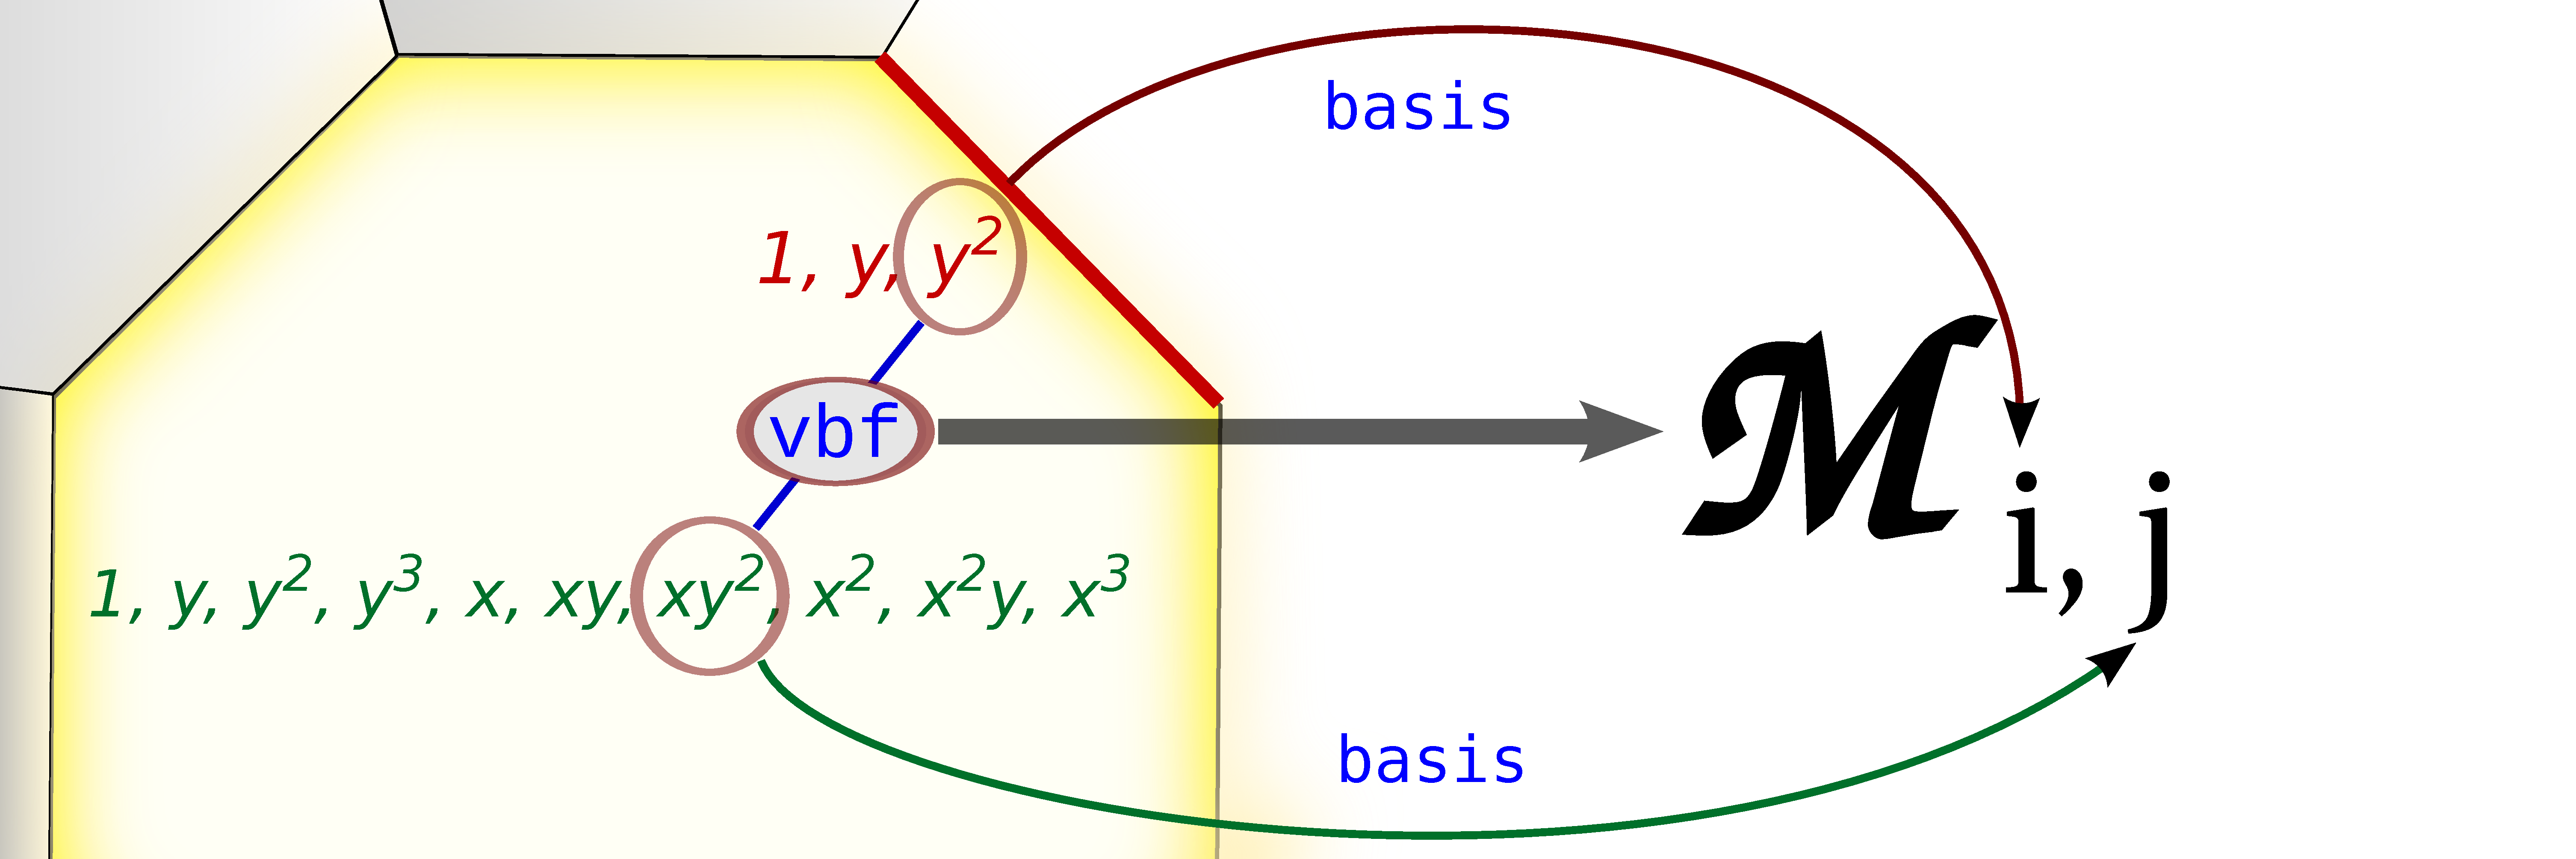
\includegraphics[width=11cm, height=3.6666cm]{img/sysmatrix_local_basis_vs_basis_practical.pdf}}

  \vspace{.15cm}
  Instead, we traverse the local representations of the basis elements, and only compute vbf values for ``nearby'' basis  
  elements according to their local representations.
  
  \pause
  \vspace{.15cm}
  When a calculation is done for a pair of local basis element representations, we can then translate the local representations
  to the global numbering via the \texttt{\textcolor{blue}{basis}} object, to fill spots in the system matrix, which will be a
  sparse matrix.
\end{frame}

\begin{frame}
  \frametitle{The System Matrix -- Pre-Computing Interactions}
  
  Since our vbf is defined in terms of interactions on single oriented shapes, thanks to the \emph{locality} and
  \emph{element-summability} assumptions, we can \emph{\textbf{pre-compute vbf values}} between shape functions on the same
  oriented shape, for each oriented shape, before building the matrix.
  
  \pause
  \vspace{.2cm}
  \textbf{Oriented Shapes and their Shape Functions}
 
  \vspace{.1cm}
  We first must collect the basic information about each oriented shape and its shape functions, for each oriented shape number up to
  \texttt{\small \textcolor{blue}{mesh.\textcolor{orange}{num\_oriented\_element\_shapes}()}}:
  \vspace{.15cm}

  \pause
  -- From the basis, we get the per-interior shape function monomials,\\ 
  \hspace{0.5cm}\texttt{\small \textcolor{blue}{basis.\textcolor{orange}{ref\_int\_mons}()}}
    
  \pause
  -- From the mesh we get the number of side faces for the oriented shape,\\ 
  \hspace{0.5cm}\texttt{\small \textcolor{blue}{mesh.\textcolor{orange}{num\_side\_faces\_for\_shape}(oshape)}}

  \pause
  -- For each side face of the shape, from the basis we fetch the sequence of shape function monomials supported on the shape side,\\
  \hspace{0.5cm}\texttt{\small \textcolor{blue}{basis.\textcolor{orange}{side\_mons\_for\_oshape\_side}(oshape, side\_face)}}
\end{frame}

\begin{frame}
  \frametitle{The System Matrix -- Pre-Computing Interactions (Contd)}
  Now we can compute and store vbf values for each pair of shape functions on each oriented shape, prior to filling the system matrix.
  
  \pause
  \frame{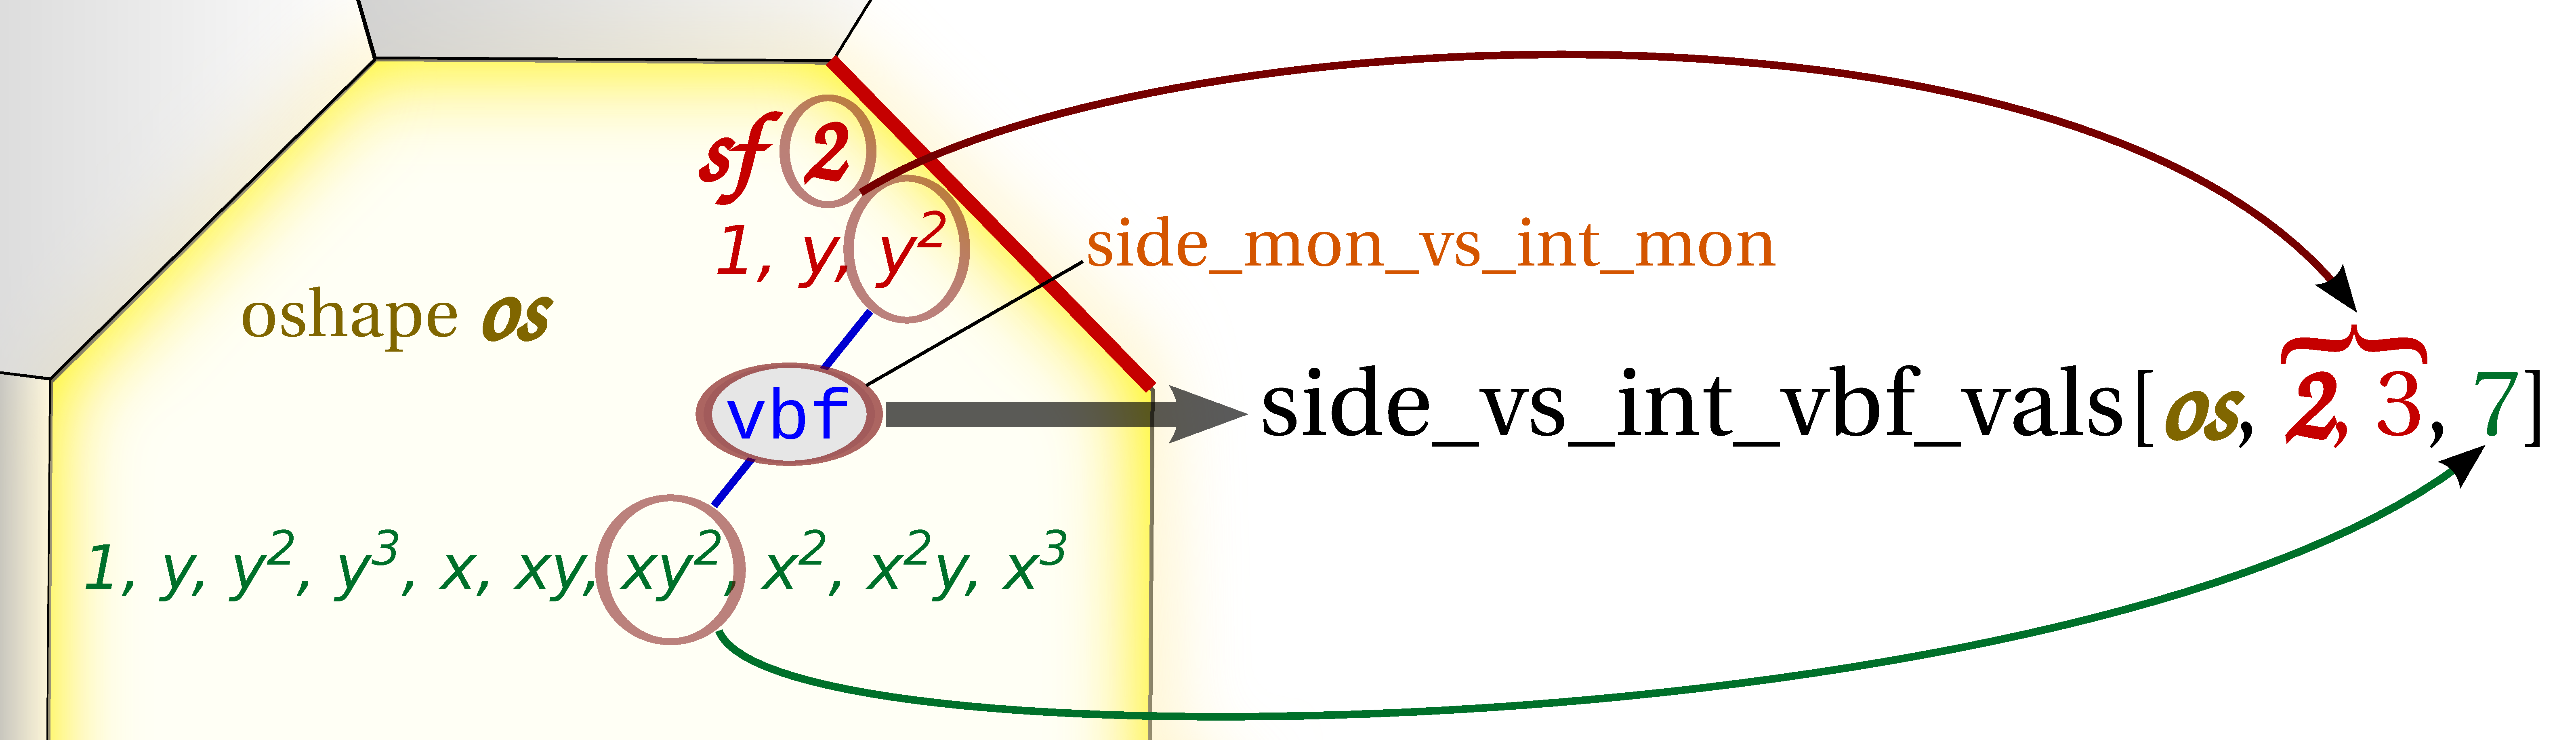
\includegraphics[width=11cm, height=3.1574cm]{img/sysmatrix_precomputed_interactions.pdf}}

  \pause
  \vspace{0.15cm}
  In each case we use the matching vbf function for the types of shape functions being paired.  For example for
  a side-supported vs interior-supported pairing (shown), we apply the vbf contract function\\
  \texttt{\small \textcolor{blue}{vbf.\textcolor{orange}{side\_mon\_vs\_int\_mon}(oshape, side\_monn, sf, int\_monn)}}.

  The pre-computed results are stored by oriented shape, side faces and monomial numbers.
\end{frame}

\begin{frame}
  \frametitle{The System Matrix -- Interior Elements vs Interior Elements}
  \vspace{-.2cm}
  \texttt{\textbf{for} \textcolor{blue}{fe} \textbf{in} $\{1,\dots,$\textcolor{blue}{mesh.\textcolor{orange}{num\_fes}()}$\}$\\
    \hspace{0.2cm} let \textcolor{blue}{oshape} = \textcolor{blue}{mesh.\textcolor{orange}{oriented\_shape\_for\_fe}(fe)}\\
    \hspace{0.2cm} \textbf{for} \textcolor{blue}{monn\_1}, \textcolor{blue}{monn\_2} in
                        $\{1,\dots,$\textcolor{blue}{basis.\textcolor{orange}{mons\_per\_fe\_int}()}$\}$\\
    \hspace{0.6cm}  let \textcolor{blue}{i} = \textcolor{blue}{basis.\textcolor{orange}{int\_mon\_el\_num}(fe, monn\_1)}\\
    \hspace{0.6cm}  let \textcolor{blue}{j} = \textcolor{blue}{basis.\textcolor{orange}{int\_mon\_el\_num}(fe, monn\_2)}\\
    \hspace{0.6cm}  \textcolor{blue}{$M_{i,j}$} = \textcolor{blue}{int\_vs\_int\_vbf\_vals[oshape, monn\_2, monn\_1]}
  }
  \frame{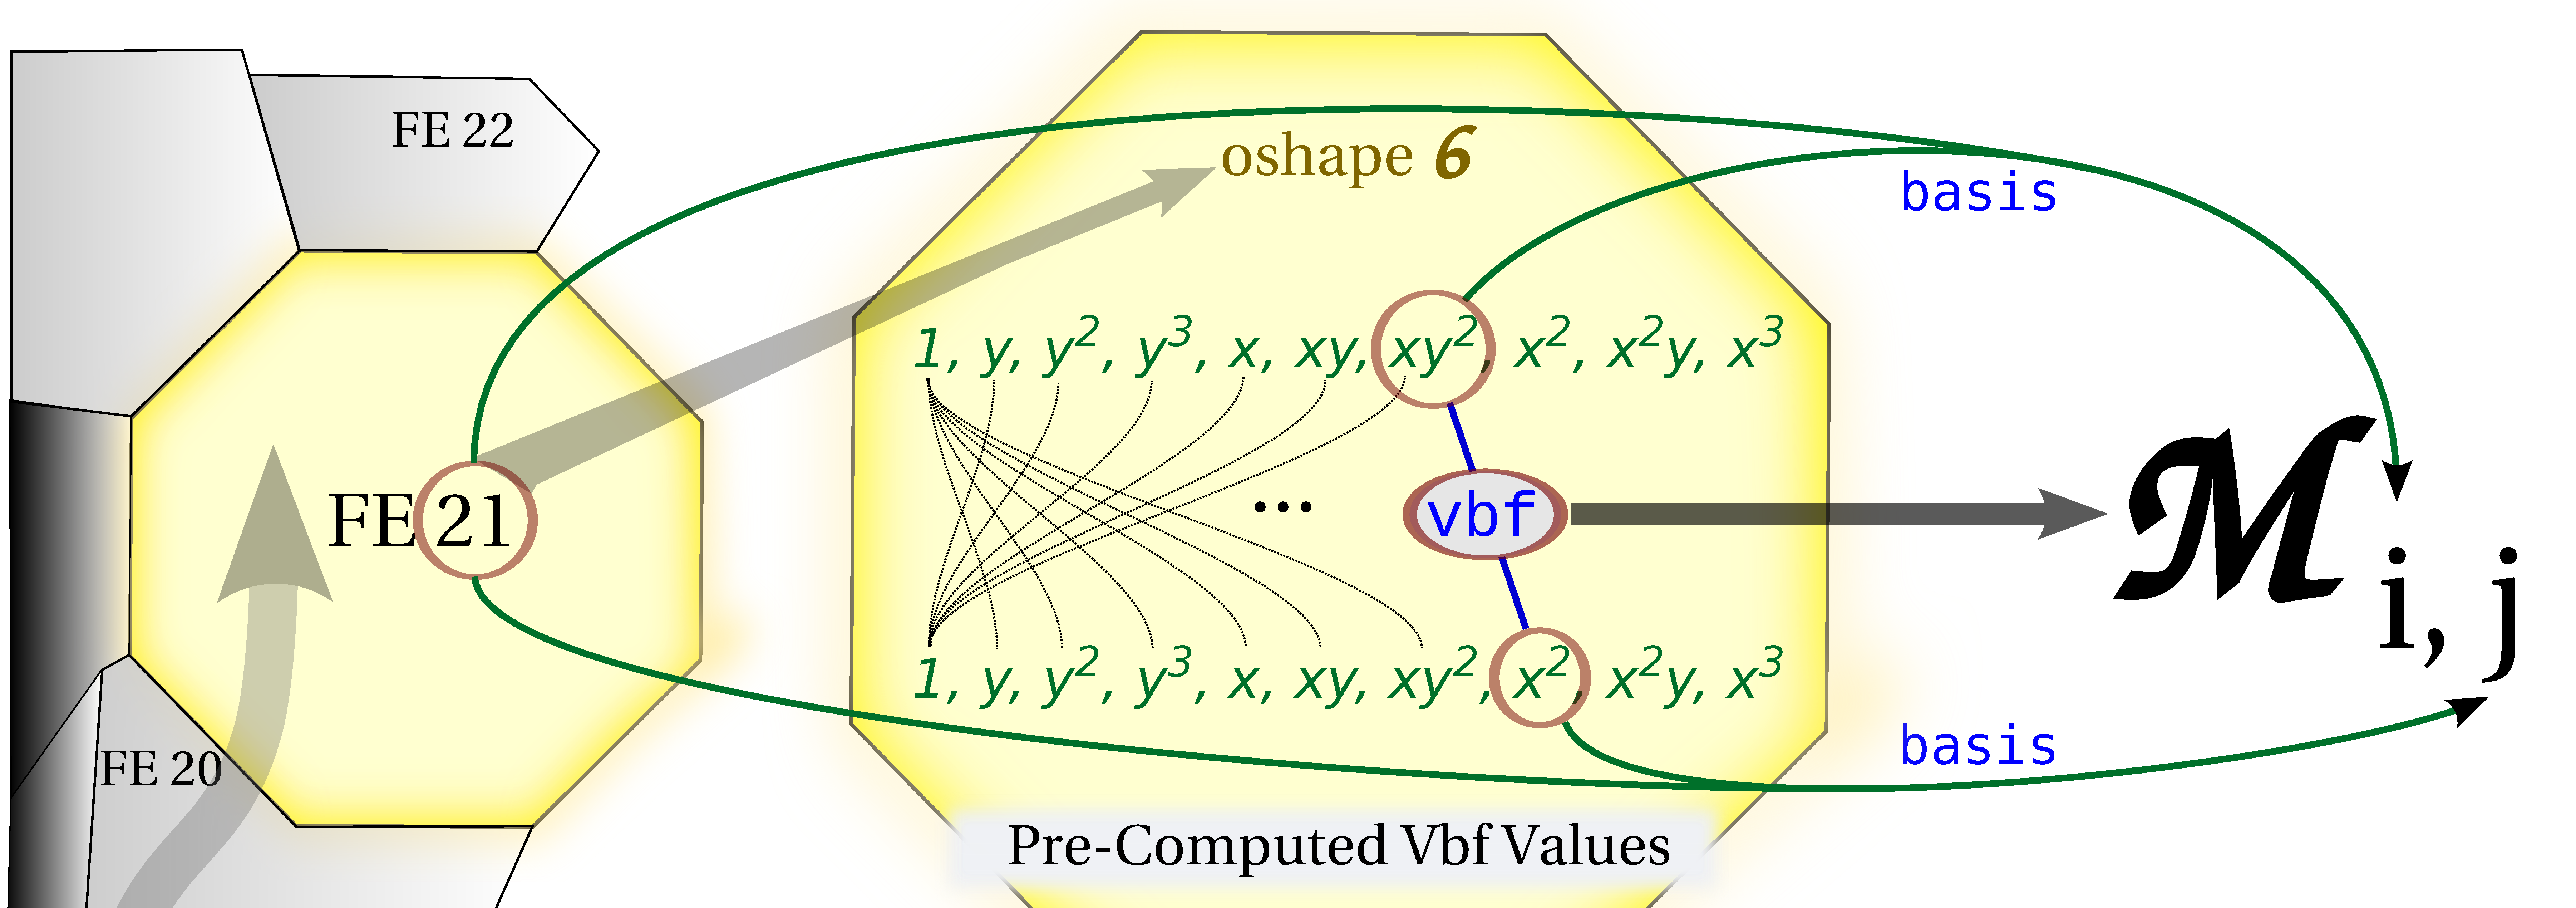
\includegraphics[width=11.5cm, height=4.2295cm]{img/sysmatrix_int_vs_int.pdf}}
  \pause
  Here per-element vbf values are complete $\mathfrak{a}$ values by the locality prop.
\end{frame}

\begin{frame}
  \frametitle{The System Matrix -- Side Elements vs Interior Elements}
  \texttt{\textbf{for} \textcolor{blue}{fe} \textbf{in} $\{1,\dots,$\textcolor{blue}{mesh.\textcolor{orange}{num\_fes}()}$\}$\\
    \hspace{0.2cm} let \textcolor{blue}{oshape} = \textcolor{blue}{mesh.\textcolor{orange}{oriented\_shape\_for\_fe}(fe)}\\
    \hspace{0.2cm} \textbf{for} \textcolor{blue}{monn\_1} in 
                     $\{1,\dots,$\textcolor{blue}{basis.\textcolor{orange}{mons\_per\_fe\_int}()}$\}$,\\
    \hspace{1.0cm} \textcolor{blue}{sf} in $\{1,\dots,$\textcolor{blue}{mesh.\textcolor{orange}{num\_side\_faces\_for\_shape}(oshape)}$\}$,\\
    \hspace{1.0cm} \textcolor{blue}{monn\_2} in 
                     $\{1,\dots,$\textcolor{blue}{basis.\textcolor{orange}{mons\_per\_fe\_side}()}$\}$\\
    \hspace{0.6cm}  let \textcolor{blue}{i} = \textcolor{blue}{basis.\textcolor{orange}{int\_mon\_el\_num}(fe, monn\_1)}\\
    \hspace{0.6cm}  let \textcolor{blue}{j} = \textcolor{blue}{basis.\textcolor{orange}{fe\_side\_mon\_el\_num}(fe, sf, monn\_2)}\\
    \hspace{0.6cm}  \textcolor{blue}{$M_{i,j}$} = \textcolor{blue}{side\_vs\_int\_vbf\_vals[oshape,sf,monn\_2,monn\_1]}
  }
  \frame{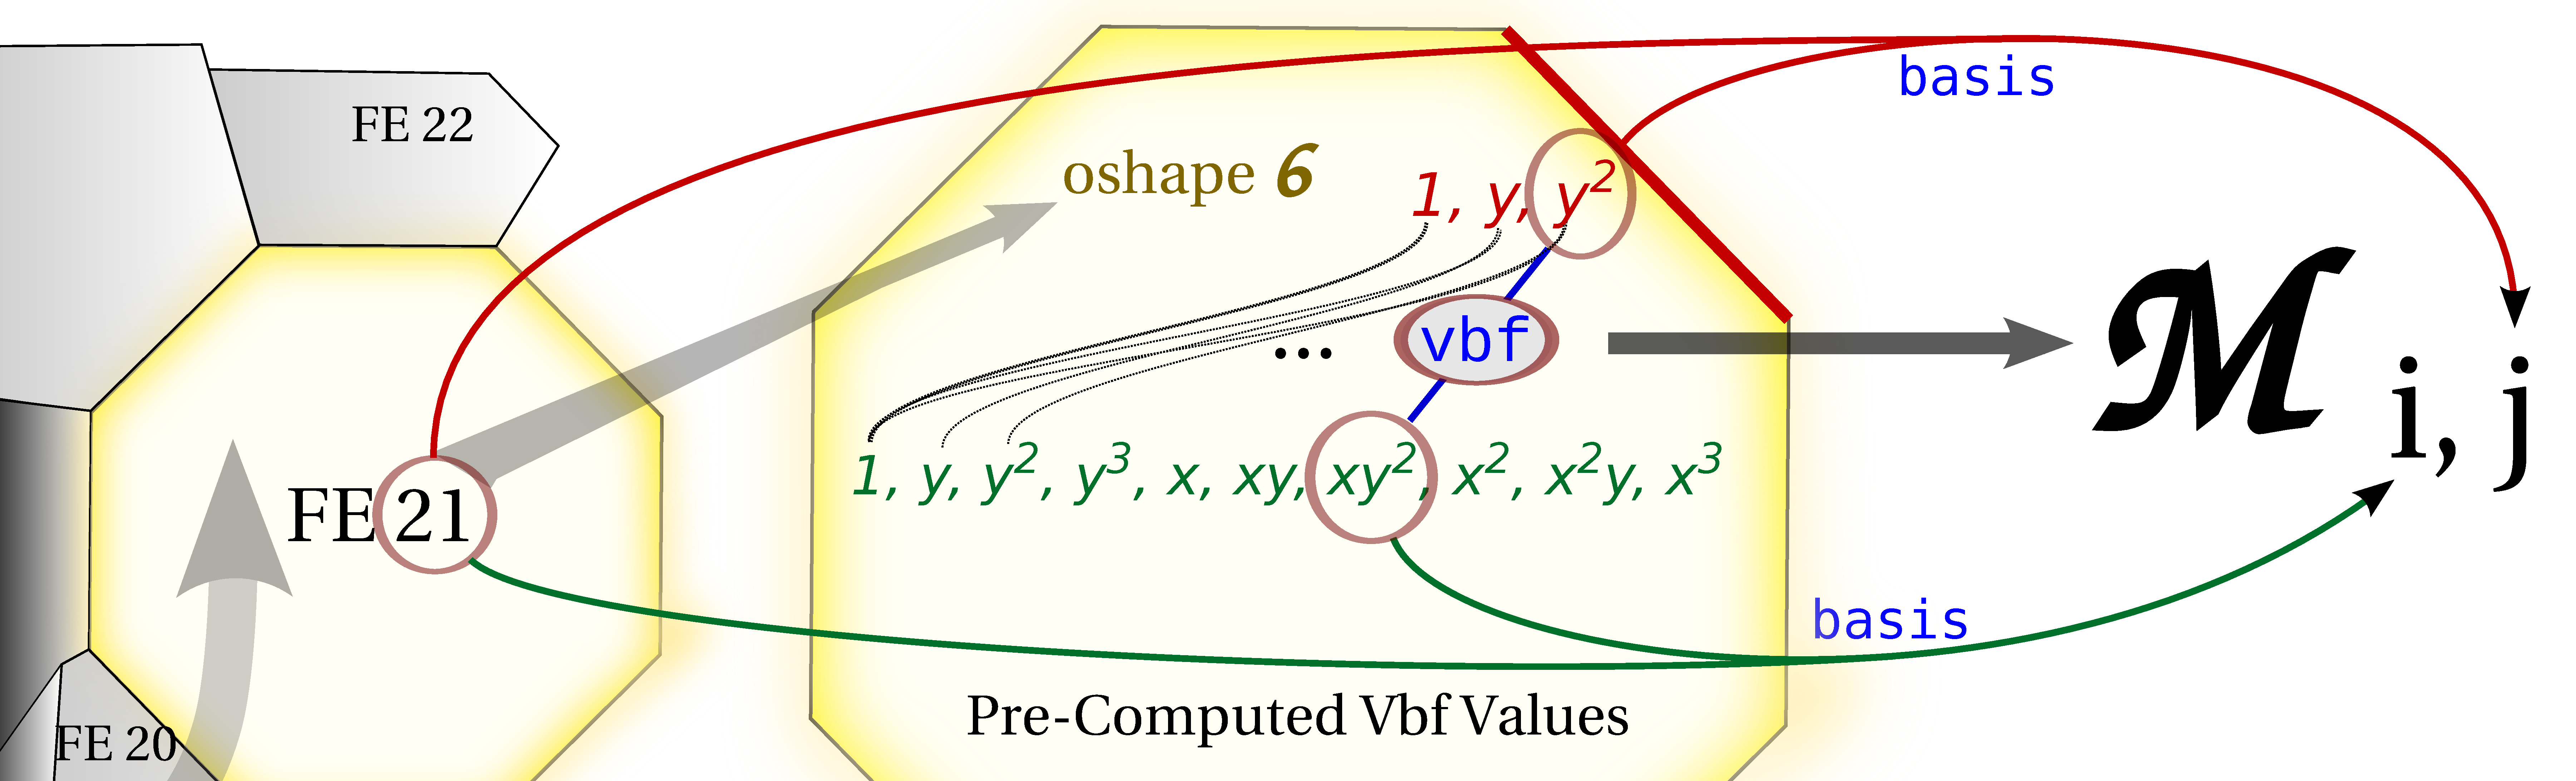
\includegraphics[width=11.5cm, height=3.4877cm]{img/sysmatrix_side_vs_int.pdf}}
  \pause
  Interior elements vs. side element entires are handled in a similar way.
\end{frame}

\begin{frame}
  \frametitle{The System Matrix -- Side Elements vs Interior Elements}

  All cases so far have yielded the total vbf $\mathfrak{a}$ value for a pair of shape functions by evaluating our per-element vbf
  \texttt{\textcolor{blue}{vbf}} $\phi$ on only a single finite element. This is because when either argument to $\phi$ is an
  interior supported shape function, then there can only be one finite element that includes both shape function supports.

  \pause
  \vspace{.15cm}
  However at a pair of side supported basis elements, $\phi$ can yield non-zero contributions from \emph{two} finite elements, because
  two finite elements can include both supports.

  \pause
  \vspace{.15cm}
  (Diagram of possible side vs side cases)
\end{frame}

%// Iterate basis element pairs beginning with a side supported element.
%for nbs in range(0, mesh.num_nb_sides()) {
  %// Get the representations of our nbs as the side faces of finite elements.
  %let nbs_incls = mesh.fe_inclusions_of_nb_side(nbs);

  %for monn_1 in range(0, num_side_mons) { let monn_1 = FaceMonNum(monn_1);
    %let r = *basis.nb_side_mon_el_num(nbs, monn_1);
   
    %// Iterate element pairs with our side supported element vs side supported elements.
   
    %// Loop over the non-boundary side interactions with our first side, nbs.
    %let nbs_filter = if sym { |nbs_2: NBSideNum| nbs_2 >= nbs } else { |_nbs_2| true };
    %for nb_sides_interaction in asc_nb_sides_interactions(&nbs_incls,
                                                          %nbs_filter,
                                                          %mesh,
                                                          %fe_nb_sides_buf, nb_side_interactions_buf).iter() {
      %match nb_sides_interaction {
        %&OneFESideSideInter(_, nbs_2, fe, nbs_sf_in_fe, nbs_2_sf_in_fe) => {
          %let fe_oshape = mesh.oriented_shape_for_fe(fe);
          %let monn_range_lower = if sym && nbs_2 == nbs { *monn_1 } else { 0 };
          %for monn_2 in range(monn_range_lower, num_side_mons) { let monn_2 = FaceMonNum(monn_2);
             %let c = *basis.nb_side_mon_el_num(nbs_2, monn_2);
             %let ip = self.get_side_vs_side_vbf_contr(fe_oshape, nbs_2_sf_in_fe, nbs_sf_in_fe, monn_2, monn_1,
                                                      %&side_vs_side_vbf_fe_contrs);
             %m.push(r, c, ip);
          %}
        %}
        %&TwoFESideSideInter(_, nbs_2,
                            %fe_a, nbs_sf_in_fe_a, nbs_2_sf_in_fe_a,
                            %fe_b, nbs_sf_in_fe_b, nbs_2_sf_in_fe_b) => {
          %let fe_a_oshape = mesh.oriented_shape_for_fe(fe_a);
          %let fe_b_oshape = mesh.oriented_shape_for_fe(fe_b);
          %let monn_range_lower = if sym && nbs_2 == nbs { *monn_1 } else { 0 };
          %for monn_2 in range(monn_range_lower, num_side_mons) { let monn_2 = FaceMonNum(monn_2);
            %let c = *basis.nb_side_mon_el_num(nbs_2, monn_2);
            %let ip = self.get_side_vs_side_vbf_contr(fe_a_oshape, nbs_2_sf_in_fe_a, nbs_sf_in_fe_a, monn_2, monn_1,
                                                     %&side_vs_side_vbf_fe_contrs) + 
                     %self.get_side_vs_side_vbf_contr(fe_b_oshape, nbs_2_sf_in_fe_b, nbs_sf_in_fe_b, monn_2, monn_1,
                                                     %&side_vs_side_vbf_fe_contrs);
            %m.push(r, c, ip);
          %}
        %}
      %}
    %} // side-side interactions
  %} // monn_1
%} // nbs

%m

\subsection{TODO}
\begin{frame}
  \frametitle{TODO - Sketch of Remainder}
  \begin{itemize}[<+->]
    \item Building system matrix, in detail.  Illustrate each form of interaction of elements.
    \item In depth look at two mesh implementations, triangle mesh from mesh generator, rectangle mesh.
      Esp. integration examples using mixed coordinate systems between interior and side.
  \end{itemize}
\end{frame}

\subsection{Implementing VBFs}

\begin{frame}
  \frametitle{Implementing VBFs -- Laplace on Interior/Interior Mons}
  \vspace{-.56cm}
  \begin{align*}
    \mathfrak \phi(v,w) = \spot<2->{(a \nabla_w v,\nabla_w w)_{\scriptscriptstyle T_0}} \;+\;
    h_T^{-1}\langle Q_b v_{\scriptscriptstyle T_0} - v,Q_b w_{\scriptscriptstyle T_0} - w \rangle_{\partial T}
  \end{align*}
  \texttt{\textcolor{blue}{int\_mon\_vs\_int\_mon(oshape, imonn1, imonn2)}}\\
  \pause
  \vspace{.35cm}
  \uncover<+-> {
  -- Ask the \texttt{\textcolor{blue}{basis}} for the weak gradients of the interior monomials, using
  function {\small \texttt{\textcolor{blue}{basis.\textbf{\textcolor{orange}{int\_mon\_wgrad}(monn, oshape)}}}}.
      
  \vspace{.1cm}
  \uncover<+-> {
  -- Form product $a \nabla_w m_1 \cdot \nabla_w m_2$, which is a polynomial. Polynomials can be represented as a sequence
  of $(\mathbb{R}, Monomial)$ pairs. See functions \emph{dot} and \emph{mdot} in the weak gradient source code
  \footnote{https://raw.github.com/scharris/WGFEM-Rust/master/weak\_gradient.rs} for implementation details.
       
  \vspace{.1cm}
  \uncover<+-> {
  -- Integrate the dot product polynomial over the shape's interior, using another new function for the mesh contract,\\
  \texttt{\small \textcolor{blue}{mesh.\textcolor{orange}{intg\_facerel\_poly\_on\_oshape\_int}(poly, oshape)}}.\\

  \vspace{0.4cm}
  This takes care of the first term.
  }}}
\end{frame}

\begin{frame}
  \frametitle{Implementing VBFs -- Laplace Interior/Interior Contd}
  \vspace{-.5cm}
  \begin{align*}
   \mathfrak \phi(v,w) = (a \nabla_w v,\nabla_w w)_{\scriptscriptstyle T_0} \;+\; 
   \spot<1->{h_T^{-1}\langle Q_b v_{\scriptscriptstyle T_0} - v,Q_b w_{\scriptscriptstyle T_0} - w \rangle_{\partial T}}
  \end{align*}

  \uncover<+-> {
  -- Introduce new mesh function for maximum element diameter,
     $\quad h_T = \texttt{\small \textcolor{blue}{mesh.\textcolor{orange}{max\_fe\_diameter}()}}$.
  
  \uncover<+-> {
  -- Our shape functions $v$ and $w$ are $0$ on the boundary, leaving only 
  \begin{align*}
    s(v,w) &= h_T^{-1} \langle Q_b v_{\scriptscriptstyle T_0}, Q_b w_{\scriptscriptstyle T_0} \rangle_{\partial T}\\
           &= h_T^{-1} \sum_{s \in sides(T)} \langle Q_b v_{\scriptscriptstyle T_0}, Q_b w_{\scriptscriptstyle T_0} \rangle_{s}
  \end{align*}
  
  \uncover<+-> {
  -- Here the $Q_b$ projections of the interior monomials are computed as described in the projection section.
  
  \uncover<+-> {
  -- We compute inner products to be summed using new mesh function\\
  \texttt{\small \textcolor{blue}{mesh.\textcolor{orange}{intg\_facerel\_poly\_x\_facerel\_poly\_on\_oshape\_side}\\
  \hspace{0.75cm}(poly1, poly2, oshape, side\_face)}}, and to iterate sides in the sum we use mesh function
  \texttt{\small \textcolor{blue}{mesh.\textcolor{orange}{num\_side\_faces\_for\_shape}(oshape)}}.
  }}}}
\end{frame}

\begin{frame}
  \frametitle{Implementing VBFs -- Laplace on Interior/Side Mons}
  \vspace{-1.38cm}
  \begin{align*}
    \mathfrak \phi(v,w) = \spot<2->{(a \nabla_w v,\nabla_w w)_{\scriptscriptstyle T_0}} \;+\;
    h_T^{-1}\langle Q_b v_{\scriptscriptstyle T_0} - v,Q_b w_{\scriptscriptstyle T_0} - w \rangle_{\partial T}
  \end{align*}
  
  \texttt{\small \textcolor{blue}{int\_mon\_vs\_side\_mon(oshape, imonn, smonn, side\_face)}}\\
  \vspace{.3cm}
  
  \pause
  \uncover<+-> {
  -- Again we ask the \texttt{\textcolor{blue}{basis}} for the weak gradients,
     via functions {\small \texttt{\textcolor{blue}{basis.\textbf{\textcolor{orange}{int\_mon\_wgrad}(monn, oshape)}}}} and
     {\small \texttt{\textcolor{blue}{basis.\textbf{\textcolor{orange}{side\_mon\_wgrad}(monn, oshape, side\_face)}}}}.\\
  -- We use the mesh for the integration as before via
     \texttt{\small \textcolor{blue}{mesh.\textcolor{orange}{intg\_facerel\_poly\_on\_oshape\_int}(poly, oshape)}}.\\
  
  \vspace{.3cm}
  \uncover<+-> {
  -- Note: Though the integration in the first term is over the interior, that does \emph{\textbf{not}} mean that the result
  is 0 just because one of the shape functions is 0 throughout the interior. Side supported elements often have weak gradients
  which are non-zero on the interior of the element.
  }}
\end{frame}

\begin{frame}
  \frametitle{Implementing VBFs -- Laplace Interior/Side Mons (Contd)}
  \vspace{-.5cm}
  \begin{align*}
    \mathfrak \phi(v,w) = (a \nabla_w v,\nabla_w w)_{\scriptscriptstyle T_0} \;+\;
    \spot<1->{h_T^{-1}\langle Q_b v_{\scriptscriptstyle T_0} - v,Q_b w_{\scriptscriptstyle T_0} - w \rangle_{\partial T}}
  \end{align*}

  \uncover<2-> {
    With $v$ being our interior supported basis element and $w$ the side supported element, the stabilization term is
    \begin{align*}
      s(v,w) &= h_T^{-1} \langle Q_b v_{\scriptscriptstyle T_0}, -w \rangle_{\partial T}\\
             &= h_T^{-1} \langle Q_b v_{\scriptscriptstyle T_0}, -w \rangle_{s}, \; \text{ where s is the supporting side of w,}
    \end{align*}
   because $v$ is $0$ on each side, and $w$'s interior polynomial is $0$ and hence its projection $Q_b\,w$ onto the side spaces
   is also $0$.\\

  \vspace{0.1cm}
  \uncover<3-> {
  -- We obtain the projection $Q_b v_{\scriptscriptstyle T_0}$ of the interior monomial as described previously in the projection section.

  \vspace{0.1cm}
  \uncover<4-> {
  -- The inner product is computed via the new mesh integration function 
  \texttt{\small \textcolor{blue}{mesh.\textcolor{orange}{intg\_facerel\_mon\_x\_facerel\_poly\_on\_oshape\_side}\\
  \vspace{-.1cm}\hspace{1cm}(side\_mon, int\_proj, oshape, side\_face)}}.

  \vspace{0.1cm}
  \uncover<5-> {
  -- The side vs. interior function is implemented in the same way.
  }}}}
\end{frame}

\begin{frame}
  \frametitle{Implementing VBFs -- Laplace on Side/Side Mons}
  \vspace{-0.5cm}
  \begin{align*}
    \mathfrak \phi(v,w) = \spot<2>{(a \nabla_w v,\nabla_w w)_{\scriptscriptstyle T_0}} \;+\;
    \spot<3>{h_T^{-1}\langle Q_b v_{\scriptscriptstyle T_0} - v,Q_b w_{\scriptscriptstyle T_0} - w \rangle_{\partial T}}
  \end{align*}
  
  \texttt{\small \textcolor{blue}{side\_mon\_vs\_side\_mon\_fe\_contr(oshape, smonn1,sf1, smonn2,sf2)}}\\
  \vspace{.3cm}
  
  \pause
  \uncover<+-> {
  -- The first term is computed much as before, using  
     {\small \texttt{\textcolor{blue}{basis.\textbf{\textcolor{orange}{side\_mon\_wgrad}(monn, oshape, side\_face)}}}} and \\
     \texttt{\small \textcolor{blue}{mesh.\textcolor{orange}{intg\_facerel\_poly\_on\_oshape\_int}(poly, oshape)}}.\\
  
  \vspace{.1cm}
  \uncover<+-> {
  -- For the stabilization term, the interior pieces to be projected are 0, so 
  \begin{align*}
    s(v,w) &= h_T^{-1} \langle -v, -w \rangle_{\partial T} = h_T^{-1} \sum_{s \in sides(T)} \langle v, w \rangle_s\\
           &= 
        \begin{cases}
          h_T^{-1} \langle v, w \rangle_s, &\mbox{\small if $v$ and $w$ have common support side $s=sf1=sf2$}\\
          0, &\mbox{ otherwise}
        \end{cases}
  \end{align*}
  
  \vspace{.1cm}
  \uncover<+-> {
    Thus if the shape functions are supported on the same side, we use
    \texttt{\scriptsize \textcolor{blue}{mesh.\textcolor{orange}{intg\_facerel\_mon\_on\_oshape\_side}(smonn, oshape, side\_face)}}
    for the integration, where \texttt{\small \textcolor{blue}{smonn}} is the product of the side monomials, else $0$.
  }}}
\end{frame}

\begin{frame}
  \frametitle{Implementing VBFs -- Symmetry}
  \begin{align*}
    \mathfrak \phi(v,w) = (\spot<2->{a} \nabla_w v,\nabla_w w)_{\scriptscriptstyle T_0} \;+\;
    h_T^{-1}\langle Q_b v_{\scriptscriptstyle T_0} - v,Q_b w_{\scriptscriptstyle T_0} - w \rangle_{\partial T}
  \end{align*}
  
  \texttt{\small \textcolor{blue}{is\_symmetric()}}\\
 
  \pause
  \uncover<+-> {
  \vspace{0.5cm}
  Yes if the matrix \spot<2->{$a$} is provided, else no.
 
  \uncover<+-> {
  \vspace{0.3cm}
  -- It is always OK to answer no.
  
  \uncover<+-> {
  \vspace{0.3cm}
  -- Yes answer enables more efficient algorithms.
  }}}
\end{frame}

\begin{frame}[fragile]
  \frametitle{Implementing VBFs -- Summary}
  \uncover<+-> {
  Alternate equations are relatively easy to support. Only four non-trivial vbf contract functions need to be written (bottom),
  which are relatively simple and also similar to each other.\\
  }
  \begin{Verbatim}[gobble=2, commandchars=\\\{\}, fontsize=\tiny, fontfamily=tt]
  fn \textcolor{green!40!black}{ip_wgrads_term}(&self, wgrad_1: &WeakGrad, wgrad_2: &WeakGrad, oshape: OShape) -> R \{
    let wgrads_prod = unsafe \{
      match self.left_wgrad_multiplier \{
        Some(ref m) => cast::transmute_mut(self).weak_grad_ops.mdot(m, wgrad_1, wgrad_2),
        None => cast::transmute_mut(self).weak_grad_ops.dot(wgrad_1, wgrad_2)
      \}
    \};
    self.basis.\textcolor{blue}{mesh}().\textcolor{orange}{intg_facerel_poly_on_oshape_int}(&wgrads_prod, oshape)
  \}

  fn \textcolor{blue}{int_mon_vs_int_mon}(&self, oshape: OShape, monn_1: FaceMonNum, monn_2: FaceMonNum) -> R \{
    let (basis, mesh) = (self.basis(), self.basis().mesh());
    let ip_wgrads_term = self.\textcolor{green!40!black}{ip_wgrads_term}(basis.int_mon_wgrad(monn_1, oshape), basis.int_mon_wgrad(monn_2, oshape), oshape);
    let h_inv = \textcolor{blue}{mesh}.\textcolor{orange}{shape_diameter_inv}(oshape);
    let stab_term = h_inv * range(0, \textcolor{blue}{mesh}.\textcolor{orange}{num_side_faces_for_shape}(oshape)).map(|sf| \{
      let projs = &self.int_mon_side_projs[*oshape][sf];
      \textcolor{blue}{mesh}.\textcolor{orange}{intg_facerel_poly_x_facerel_poly_on_oshape_side}(&projs[*monn_1], &projs[*monn_2], oshape, SideFace(sf))
    \}).sum();
    ip_wgrads_term + stab_term
  \}
  \end{Verbatim}
\end{frame}

  
\end{document}

